%!TEX TS-program = xelatex
%!TEX encoding = UTF-8 Unicode
%!BIB program = bibtex

\documentclass[oneside, 11pt, letterpaper]{marl}

\title{\doublespacing
%Applications of Generative Neural Networks \\ in Automatic Music Transcription\\
Automatic Music Transcription in the Deep Learning Era:\\Perspectives on Generative Neural Networks\\{\textcolor{red}{[A draft compiled on \today]}}
}

\threecommittee
{Professor Juan Pablo Bello, Chairperson}
{Professor Robert Rowe}
{Doctor Eric J. Humphrey}

\degree{Doctor of Philosophy}
\degreedate{\the\year}

\author{\href{mailto:jongwook@nyu.edu}{Jong Wook Kim}}
\program{Program in \href{http://steinhardt.nyu.edu/music/technology/}{Music Technology}}
\department{Department of \href{http://steinhardt.nyu.edu/music/}{Music and Performing Arts Professions}}
\university{\href{http://www.nyu.edu/}{New York University}}
\crest{}%\includegraphics[width=3in]{NYUlogoLarge2597}}
\submittedtext{Submitted in partial fulfillment\\
  of the requirements for the degree of\\
  Doctor of Philosophy in the\\
  \href{http://steinhardt.nyu.edu/}{Steinhardt School of Culture, Education, and Human Development}}

% turn of those nasty overfull and underfull hboxes
\hbadness=10000
\hfuzz=50pt
\makeindex

\begin{document}

\sloppy
\widowpenalty=10000
\clubpenalty=10000

%: ----------------------- generate cover page ------------------------
%\setstretch{1.2}
\maketitle  % command to print the title page with above variables
% \makecopyright

% Thesis Abstract -----------------------------------------------------


%\begin{abstractslong}    %uncommenting this line, gives a different abstract heading
\begin{abstracts}        %this creates the heading for the abstract page

Put your abstract or summary here, if your university requires it.

\end{abstracts}
%\end{abstractlongs}


% ---------------------------------------------------------------------- 


\doublespacing
% % Thesis Dedictation ---------------------------------------------------

\begin{dedication} %this creates the heading for the dedication page

To the Flying Spaghetti Monster.

\end{dedication}

% ----------------------------------------------------------------------

% 
% this file is called up by thesis.tex
% content in this file will be fed into the main document

\chapter*{Acknowledgements}

Sweet sweet sweet roll croissant candy souffle pie chocolate bar.
Pudding candy carrot cake sweet halvah. 
Ice cream ice cream tiramisu jelly-o chupa chups chupa chups carrot cake. 
Donut tootsie roll pie pudding icing muffin candy canes. 
Cupcake tootsie roll croissant chocolate applicake croissant macaroon gummi bears. 
Muffin icing icing toffee jelly beans toffee lemon drops. 
Cookie chocolate cake topping carrot cake chocolate bar jujubes sweet roll.

\singlespacing

%: ----------------------- contents ------------------------
% levels are: 0 - chapter, 1 - section, 2 - subsection, 3 - subsubsection
\setcounter{secnumdepth}{3} % organisational level that receives a numbers (NYU Steinhardt recommends level 0, which is pretty hideous)
\setcounter{tocdepth}{1}    % print table of contents for level 2

{
	\small 
	\tableofcontents            % print the table of contents
	%\addcontentsline{toc}{section}{continued}
	%: ----------------------- list of figures/tables ------------------------
	
	%\clearpage
	%\listoftables                   % print list of tables
	\clearpage
	\listoffigures                  % print list of figures
}

\chapterbegin

% % this file is called up by thesis.tex
% content in this file will be fed into the main document

\newacronym{tcap}{TCAP}{Toffee chocolate apple pie}


\newglossaryentry{Chupa chups}
{
  name={chupa chups},
  description= {Powder fruitcake ice cream ice cream brownie biscuit ice cream ice cream}
}


\chapter*{}

\begin{quote}
``Marshmallow wafer oat cake carrot cake sugar plum gummi bears jujubes marzipan.''

\end{quote}

\vspace{1in}
\hspace{2in}
-Willy Wonka, {\it Midnight in the Garden of Good and Evil.}

\mainmatter
\doublespacing

%: ----------------------- subdocuments ------------------------
%!TEX root = ../dissertation.tex
% this file is called up by thesis.tex
% content in this file will be fed into the main document

%: ----------------------- introduction file header -----------------------
% the code below specifies where the figures are stored
\graphicspath{{1-introduction/figures/}}

\chapter{Introduction}
\label{ch:introduction}

As listening is a core constituent of human perception, an essential component of artificial intelligence is \emph{machine listening}.
The purpose of machine listening research is to enable computers to process and understand sounds as humans do.
In recent years, there have been an unprecedented amount of successes in the field of \emph{machine learning}, a near-synonym to artificial intelligence with a connotation of statistical and/or probabilistic methodologies, which redefined what a computer vision or natural language processing systems can do and made previously unimaginable applications such as autonomous driving and a superhuman StarCraft-playing AI into reality.

In this context, this thesis focuses on improving the machine understanding of music in order to automatically transcribe music, which largely remains an unsolved problem despite decades of research.
The recent rapid development in \emph{deep learning} research, however, hints at many new possibilities for improving the performance or even achieving human-level accuracy in music transcription.

\section{Statement of Problem}\label{sec:statement}

\begin{figure}
	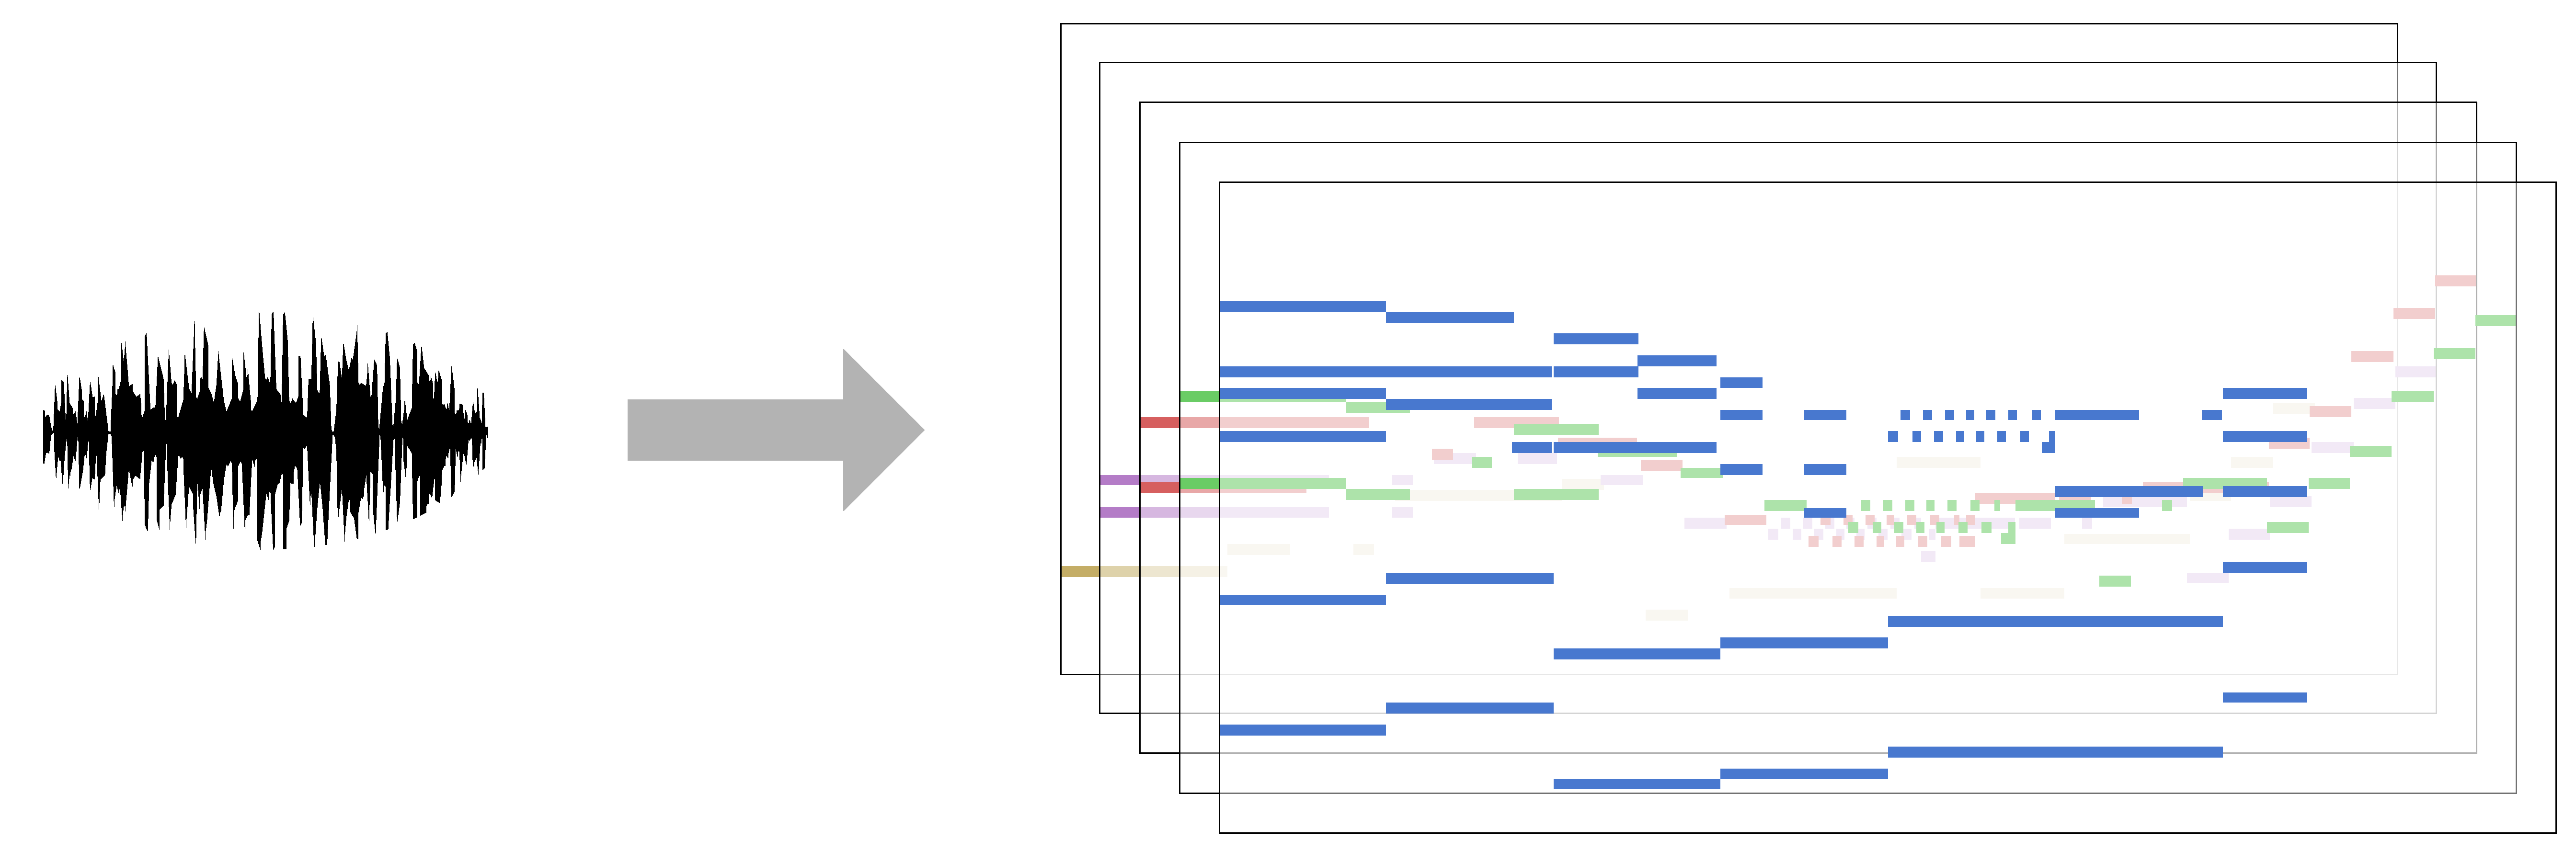
\includegraphics[width=\textwidth]{march-transcription.pdf}
	\caption{The automatic music transcription setup to be used in this thesis. Using per-instrument piano-roll representations is easier for machines to process, and avoids variability and subjectivity that may arise from symbolic and textual notations.} 
	\label{fig:transcription-to-piano-rolls}
\end{figure}

\emph{Automatic music transcription} (AMT) refers to an automated process that can identify musical events in the input audio and convert them into musical notations.
Historically, the definition of automatic music transcription varied by author, usually in terms of the form of the output representation.
In earlier works \cite{moorer1977transcription,piszczalski1977transcription}, the final output of the transcription system was to be the common music notation, i.e. a score, while later literature generalizes the problem by defining it as ``the analysis of an acoustic musical signal so as to write down the pitch, onset time, duration, and source of each sound that occurs in it" \cite{klapuri2006transcription} or ``the process of converting an acoustic musical signal into some form of musical notation" \cite{benetos2013amt}.
This thesis adopts per-instrument piano-rolls as the resulting representation of automatic music transcription, as shown in Figure \ref{fig:transcription-to-piano-rolls}, and defers the ``piano-roll to score" conversion as an out-of-scope task, which involves higher-level nontrivial tasks such as tempo and meter tracking, key signature detection, and music structure identification.
This can be justified since it allows the transcription model to focus on source separation and multi-pitch tracking, which are already highly challenging problems \cite{cemgil2006generative}.


To perform automatic music transcription, various properties of musical events, such as pitch, timbre, harmony, beats, etc., need to be defined and extracted from the audio.
In this sense, the setup of AMT is \emph{discriminative} in nature, meaning that it aims to identify different attributes from given audio, as opposed to \emph{generative} models concerning how to construct audio signals according to given conditions about those attributes.
Meanwhile, when a generative model is jointly trained with an encoder, it can learn to generate data samples from a small number of latent factors, while the encoder learns to extract those factors from the audio in a compact representation, as depicted in Figure \ref{fig:autoencoder}.
Recently, with the increased capacity of machine learning models and hardware, many \emph{deep generative models} have been proposed and shown to be capable of processing high-dimensional multimedia data.
Furthermore, significant research efforts have been made towards learning disentangled representation of data, meaning that the latent factors contain meaningful information that can be easily separated and isolated.
To this end, the goal of this thesis is to study representation learning methods powered by deep generative models, to obtain disentangled information from audio signals that can achieve better performance in music transcription.

\begin{figure}[t]
	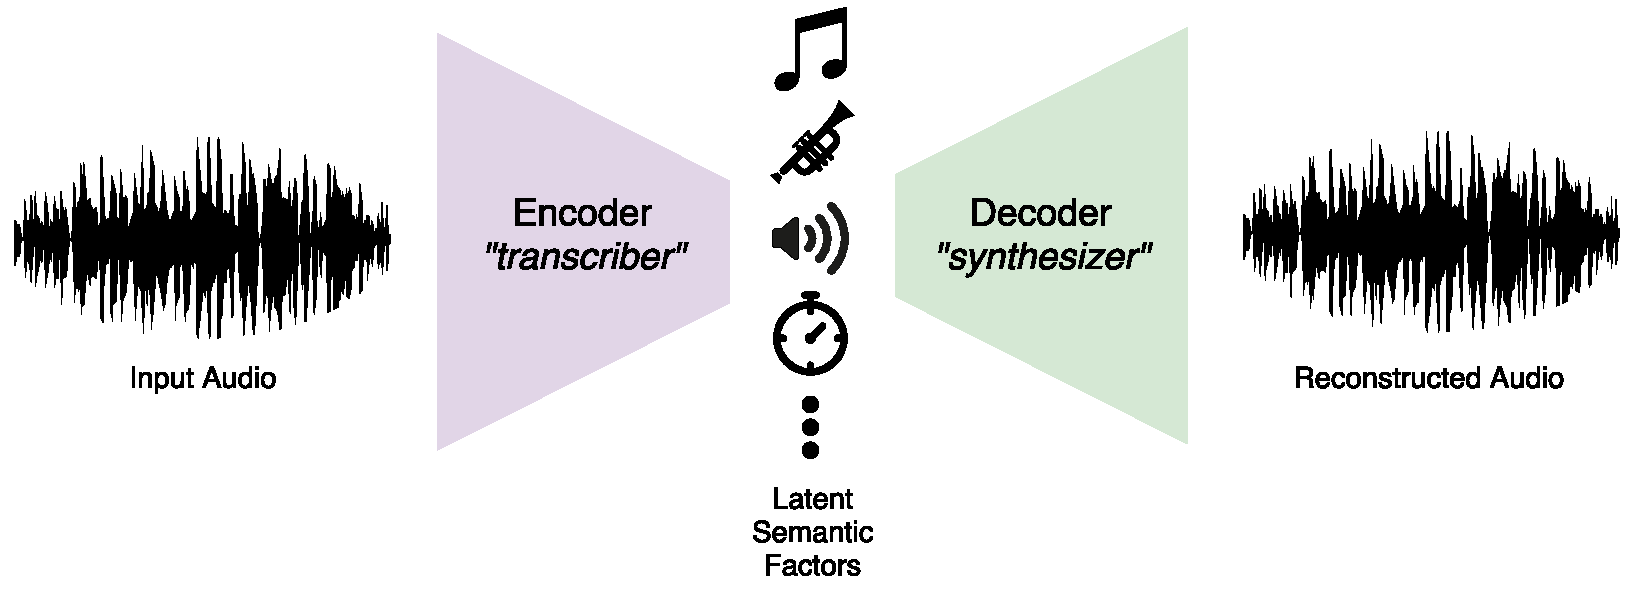
\includegraphics[width=\textwidth]{autoencoder.pdf}
	\caption{A generative model has to know all of necessary information required to reconstruct the audio data, including pitch, timbre, loudness, and duration. Generative models can be jointly trained with an encoder that finds those semantic information, giving a transcriber-synthesizer pair.}
	\label{fig:autoencoder}
\end{figure}

\section{Research Questions}\label{sec:subproblems}

To achieve the goal of improving music transcription with generative models, several research questions needs to be addressed. This thesis considers the following questions regarding the proposed approach towards automatic music transcription.

\vspace{1em}

\begin{enumerate}
\item What kinds of deep models and representations can be used for effectively extracting pitch from audio?
\item How does the choice of datasets affect the accuracy and the generalizability of a trained model?
\item How can we encode the concept of timbre in a way that is useful for music synthesis and transcription?
\item How can a transcription model make informed predictions incorporating the knowledge of music theory?
\item Can a music synthesizer component based on a deep generative model be used to improve music transcription?
\end{enumerate}

\vspace{1em}

We aim to address each of these questions in the technical chapters of the thesis.
Through extensive experimental analysis in each chapter, we draw the conclusion on the effectiveness of deep generative models in the context of automatic music transcription.


\section{Limitations}\label{sec:limitations}

Because of the sophisticated and open-ended nature of automatic music transcription, it is necessary to define the scope of the tasks and data that this thesis will be concerned with.
The purpose of this section is to define those limitations in terms of the scope of music that the proposed AMT system can process, the required capability of symbolic music processing, and the need for perceptual studies regarding the validity of AMT systems.


\subsection{Scope of Music}

Music signals typically contain both harmonic and percussive sources. 
From a signal processing point of view, harmonic sounds are quasi-periodic and contain energy only at certain frequencies, roughly at the multiples of the fundamental frequency, whereas percussive or highly inharmonic sounds have aperiodic frequency spectra in which it is not possible to define a fundamental frequency.
Consequently, transcription models for harmonic sounds and percussive sounds require different techniques according to their nature.


This thesis will limit the focus on the transcription of harmonic sounds and therefore use the per-instrument piano roll notation (Figure \ref{fig:transcription-to-piano-rolls}) as the output representation.
This is a realistic trade-off to make, because of a number of reasons.
First, learning to simultaneously model harmonic and percussive sounds is a harder problem both conceptually and computationally.
Secondly, it is possible to plug a harmonic-only model into a pipeline consisting of HPSS (harmonic-percussive source separation) and a percussion transcription model as an alternative to a comprehensive approach.
Lastly, polyphonic transcription is considered to be the most difficult problem in the domain of automatic transcription, and it is sensible to tackle this as a standalone problem in the simplest possible setup.
Excluding percussive sounds will disallow using most of pop music tracks as-is, but multi-track datasets can still be utilized since they contain each track separately.


Additional limitations should be considered on the types of the instruments and their sound variations.
Depending on the instrument, the same score could be performed using a variety of expressive techniques, such as vibrato, tremolo, pizzicato, and the usage of mutes or harmonics, among others.
In order to accurately produce a piano roll transcription that is invariant to such techniques, the model has to be trained to classify them as nonessential information, requiring the availability of datasets with the annotations for those techniques.
While an ideal model should learn those concepts as humans do, too much timbral or temporal variation for an instrument will prevent the model from learning a consistent representation corresponding to the instrument.
Therefore, for the immediate purpose of this thesis, distributions of music signals that do not contain too much of said variations will be employed.


\subsection{Symbolic Processing of Notes}

As mentioned and justified in the problem statement (Section \ref{sec:statement}), by choosing per-instrument piano rolls as the output of transcription, concerns of symbolic music processing such as beat quantization and score typesetting are excluded from the scope of this study.
The difference between a piano roll output and a full human-readable score output becomes apparent when we compare the piano rolls in Figure \ref{fig:transcription-to-piano-rolls} with Figure \ref{fig:wedding-march-score}, which is the original score from which the piano rolls are plotted.
There are many aspects in producing the score output that are highly subjective and difficult to derive a consistent evaluation metric from, such as the interpretation of legatos or staccatos and the aesthetic choices for typesetting, providing an additional justification for using the piano roll notation.


\begin{figure}
	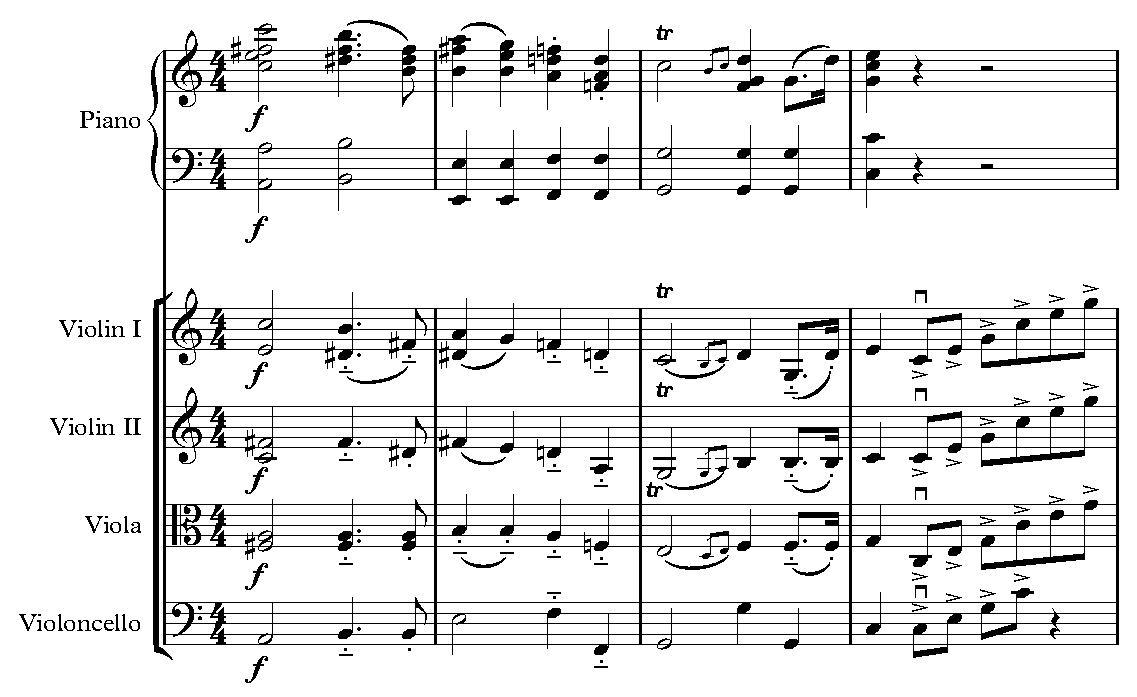
\includegraphics[width=\textwidth]{march-score.pdf}
	\caption{The full score notation of the music used to build the piano rolls in Figure \ref{fig:transcription-to-piano-rolls}. To fully recover this level of notations from the audio, the transcriber has to make many additional decisions than for the piano rolls, such as determining the key signature, time signature, clefs, dynamics, trills, bowing instructions, etc.}\label{fig:wedding-march-score}
\end{figure}


The MIDI file format is suitable for encoding data equivalent to per-instrument piano rolls, consisting of multiple tracks of \texttt{note\_on} and \texttt{note\_off} events with the corresponding timestamps.
MIDI will therefore be a supported output format of the proposed AMT system in addition to the piano roll representations, which can also be conveniently played back by media player software.
Music typesetting software such as Sibelius or Finale can render a MIDI file into score notation using the metadata in the file as well as some heuristics for beat quantization.
However, the readability of the score rendered from a transcribed MIDI file is limited, due to imperfect transcription and the absence of metadata such as the time and key signature.



\subsection{On the Need for Perceptual Studies}

This study of automatic music transcription is entirely quantitative and does not involve subjective tests on human participants.
We only aim to discover the systematic relations between audio signals and corresponding note sequences present in the datasets we use for training.
However, music is essentially a perceived notion, and thus are the core qualities of sound --- pitch, timbre, and loudness --- which are the output of automatic transcription.
For this reason, manually annotating polyphonic music is an error-prone process, where any two annotators may produce drastically different annotations.
Although this problem of inaccuracy and subjective difference is often overcome by using a ground-truth dataset synthesized from known frequency information, the gap still persists between what a model can learn from synthesized audio and how it will respond to real-world sounds.
This thesis uses both kinds of datasets, from synthesized and recorded audio signals, and thus the real-world applicability of each of the proposed models should be carefully examined.

The goal of automatic transcription is at a lower level than for tasks such as  chord recognition and melody tracking, which may incur even more subjective disagreements caused by the imprecise definitions of chords and melodies.
Being directly related to the physical concept of fundamental frequency, pitch is relatively precisely defined in this sense, and formulating automatic music transcription as an audio-to-piano-roll conversion mostly eliminates the ambiguity that exists in chord recognition and melody tracking.
There exist some cases where the mathematical definition of fundamental frequency still cannot be applied for all pitched sounds, such as the Shepard tone \cite{shepard1964circularity} where the pitch of a harmonic sound fails to be consistently mapped to a fundamental frequency.
However, disregarding these few edge cases, this study assumes that the piano roll notation can convey an objective transcription for many practical purposes, allowing us to postulate AMT as a mathematical problem which does not require experiments on human subjects.

\section{Need for Study}

The nature of music transcription is multifold; to create a complete transcription, one has to identify all instruments, onsets, dynamics, and the pitch traces for every instrument present in the music, and it would still be far from achieving the human-level accuracy.
The need for this study arises naturally, not only because this is an intriguing problem in the intersection of music and technology that has remained unsolved for decades, but also because the solution to this problem can provide practical benefits to many applications.

In order to bolster the need for this study, a few of such applications are introduced in this section, followed by discussions on the advantages of employing generative models as a means of better capturing musical semantics.
A brief perspective on AMT is presented in the context of wider AI research, followed by the organization of the chapters.


\subsection{Applications of Automatic Music Transcription}\label{sec:applications}

Many applications of the techniques in the realm of automatic music transcription is on interactive music systems.
\citeA{vercoe1984performer} proposed a quest for a \emph{synthetic performer}, which can listen, perform, and learn in the context of live performance.
Relevant sub-fields include automatic \emph{real-time accompaniment} \cite{dannenberg1985accompaniment} based on dynamic programming was one of the first successful demonstrations of AMT techniques, and \emph{Score following}, a general term referring to the synchronization of a computer with a performer playing a known score \cite{orio2003following}.
An offline music-to-score matching algorithm can also be applied to intelligent audio editors \cite{dannenberg2003following}.

\emph{Music recommender systems} can combine many kinds of information for improved music retrieval and personalization \cite{celma2010music}.
Content-based music recommender systems can utilize not only the metadata but also the audio content, and methods using timbral \cite{magno2008recommendation}, temporal \cite{li2007recommender}, and tonal features \cite{lu2009recommendation} have been introduced.
These music recommender systems can be further improved when the complete information on each domain is made available through AMT.

AMT system can help create databases for query-by-humming \cite{ghias1995humming} by automatically estimating melody annotations, where users can retrieve music by humming an excerpt of the song.
Such databases can also facilitate large-scale musicological analyses \cite{abdallah2015british}, as well as the development of computer-aided music composition \cite{agostini2013aid} that incorporates musicological knowledge.


\subsection{Generative Modeling for Fully Capturing Semantics}

Being ``generative'' means that a model is capable of generating new samples in the domain of the original data.
Generation in the symbolic domain creates new musical scores, and a generative model in the audio domain creates audio waveforms.
These two kinds of generative systems are familiar to computer music artists and are referred to as algorithmic composition \cite{fernandez2013ai} and sound synthesis \cite{cook2002synthesis} models.
This thesis defines the term ``generative model'' more specifically, as a model that can learn the distribution of provided data and can sample new samples in the original distribution.
This differs from the term ``generative'' used in computer music in a sense that it aims to accurately model the probability distribution and learn to regenerate the real-world audio to be used in music transcription, rather than focusing on the artistic aspects of generating new kinds of sounds and music.

By learning to generate data using fewer parameters than the scale of the dataset, a model has to discover the underlying natural features from the distribution of data.
In music transcription, these features correspond to the musical concepts such as pitch, timbre, and rhythm.
Philosophically, this idea follows what Richard Feynman once wrote on his blackboard, \emph{``What I cannot create, I do not understand''} and \emph{``Know how to solve every problem that has been solved''}.
He meant that the marker for truly understanding something is the ability to construct it completely from scratch.
Generative models are a branch of unsupervised learning, because they do not require labeled data.
\citeA{lecun2016unsupervised} introduced unsupervised learning as a cake, with supervised learning as icing and reinforcement learning as the cherry on the top, by which he meant that generative models need to predict at a much larger scale of information and should be is able to learn the ``common sense''.

\begin{figure}
	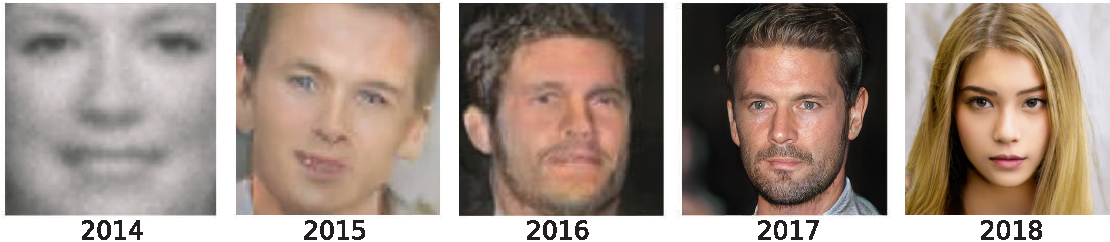
\includegraphics[width=\textwidth]{generative-evolution.pdf}
	\caption{Increasingly realistic qualities of the generated faces using generative adversarial networks as shown in \protect\cite{brundage2018malicious}; images are taken from \protect\cite{goodfellow2014gan}, \protect\cite{radford2015dcgan}, \protect\cite{liu2016cogan}, \protect\cite{karras2017pggan}, and \protect\cite{karras2019stylegan}.} 
	\label{fig:generative-evolution}
\end{figure}


Inherently, unsupervised learning is less well-defined than supervised learning, and this is the reason why unsupervised learning is sometimes synonymous with clustering, because finding clusters is usually as much an unsupervised learning system can do.
However, the recent success of deep learning introduced a new breed of generative models, enabling the end-to-end generation of complex data such as photos and audio signals.
\emph{Generative adversarial networks} (GAN) \cite{goodfellow2014gan} are the most notable among them, and their performance in generating realistic images has been improving at an extraordinary pace, as shown in Figure \ref{fig:generative-evolution}.
Combined with the various techniques for manipulating the semantic information in GANs as will be introduced in Section \ref{ch:deeplearning}.\ref{sec:gan}, this hints at completely new kinds of generative methodologies for audio processing.


In this context, this thesis aims to design and develop improved methods for automatic music transcription powered by deep generative models.
The idea specifically hypothesizes that by training a generative model, it is possible to learn disentangled representations, from which the information necessary for transcription can be easily extracted, as depicted in Figure \ref{fig:autoencoder}.
By doing so, the ultimate objective is to build an end-to-end differentiable model that connects the piano roll representation to audio signals, in order to perform automatic music transcription --- obtaining the most likely piano roll representation for given a audio waveform.


\subsection{On the Broader Context of Machine Listening in AI Research}

Using generated audio data and generative models is partly motivated by the fact that synthesized music is more prevalent and perceptually more familiar to people than synthesized texts or pictures.
Many commercial music tracks are often produced entirely using software instruments, except for the vocal parts.
This suggests that synthesized and generated audio may more accurately model the distribution of the real audio data to be transcribed.
This generative approach also aligns well with how actual musicians transcribe music, where they match given audio with their knowledge of how the instruments sound when played in a certain combination of rhythms and melodies.
Therefore it is reasonable to claim that machines should also be able to perform in a similar way, provided that a proper representation of knowledge about the music and instruments is available.

The task of automatic music transcription shares many common values with other machine learning tasks, such as image segmentation, machine translation, and speech recognition, in the sense that the core task is to build an intelligent system that can extract and process useful information conveyed in complex signals.
This is an essence of artificial intelligence (AI)
--- a system that perceives its environment and takes actions that maximizes the utility \cite{russell2009ai} --- 
where an intelligent system has to understand the semantics of complex data coming from the environment in order to perform well in its tasks.
To this end, the problem of automatic music transcription is not just an intriguing task in music technology but will also be a key component of the AI-enabled future society, constituting a musical component of the artificial general intelligence (AGI), in the form of advanced machine musicianship \cite{rowe2003musicianship}.


\subsection{Organization of The Thesis}


This thesis examines the possibility of using deep generative models to learn relevant musical concepts and inform a music transcription model to incorporate them.
There exists a rich history of research aiming at the understanding of musical sounds and automatic music transcription; to validate this claim as a feasible research direction and place this thesis in the context of this continuum of research, Chapter \ref{ch:mir} provides a review of the standard methods and the current state of the art in automatic music transcription research.
Deep learning techniques are employed as a building block throughout this thesis, and a general introduction to deep learning and deep generative models is provided in Chapter \ref{ch:deeplearning}, with a focus on generative adversarial networks.

In Chapter \ref{ch:monophonic}, we first consider a subproblem of music transcription, i.e. monophonic pitch estimation, and learn that convolutional neural networks predicting two-dimensional time-frequency representations can constitute an effective strategy, which we build and extend in the subsequent chapters.
Chapter \ref{ch:synthesis} examines the applications of deep generative models in music analysis and synthesis tasks, by introducing a WaveNet-based music synthesis model that learns a multi-dimensional timbre representation.
In Chapter \ref{ch:adversarial}, generative adversarial networks are used to apply a music language model that can help improve a piano transcription model.
In Chapter \ref{ch:timbre}, we combine the analysis and synthesis methods developed in the preceding chapters and present a multi-instrument polyphonic music transcription system.
Finally, concluding remarks are provided in Chapter \ref{ch:conclusions}.



%!TEX root = ../dissertation.tex
% this file is called up by thesis.tex
% content in this file will be fed into the main document

%: ----------------------- introduction file header -----------------------
% the code below specifies where the figures are stored
\graphicspath{{2-mir/figures/}}

\chapter{Music Information Retrieval for Transcription}
\label{ch:mir}

Being able to accurately identify all musical events from audio and transcribe them into musical notations is an essential skill for musicians as well as a paramount goal of music machine learning research.
Enabling an automatic conversion between musical audio and symbolic notations, automatic music transcription opens up many new possibilities.


Due to the complexity and difficulty of creating a completely end-to-end music transcription system, many existing approaches focus on a specific subtask of the problem \cite{casey2008mir}, e.g. extracting onsets and beats, recognizing timbre and instruments, tracking monophonic and polyphonic pitches, or separating audio sources from a mixture.
Each of these subtasks poses interesting goals and applications even without the lofty goal of end-to-end music transcription, and they are classified as subproblems of \emph{music information retrieval} (MIR).
Although this term has existed since 1960s \cite{kassler1966mir}, it was only after the late 1990s when active research on this area has spun off from computer music and computational musicology literature.
During the last two decades, numerous sophisticated and novel approaches for each of these subproblems have been introduced, that have continuously improved the performance in terms of the accuracy in predicting the correct annotations.
This chapter starts by introducing the common concepts and techniques employed in many AMT models, followed by reviews of the state-of-the-art techniques in each area of music transcription.
The purpose of this chapter is to provide a survey over the history of MIR research related to automatic music transcription, as well as to show a clear common pattern over the areas of MIR where the machine learning models have been evolving from simple heuristics based on hand-crafted features to sophisticated deep learning models with millions of parameters.
Many methods employing deep neural networks are referenced in this chapter, and the concepts and the formulation of those models such as convolutional newral networks (CNN) and recurrent neural networks (RNN) are described in detail in Chapter \ref{ch:deeplearning}.


\section{Introduction}

Audio data is huge in volume; a typical audio track contains 44,100 real-numbered samples per second, and sometimes even more.
Therefore, computational methods for extracting musical information from audio usually contains a pipeline of feature extraction stages to reduce the dimensionality and increase the interpretability of input data, as shown in Figure \ref{fig:pipeline}.
The pipeline includes a few techniques widely used in speech processing, as well as many feature extraction stages created for music-specific purposes.


While there are many MIR tasks that operate on the track level, such as music recommendation, tagging, and genre classification, most subtasks of music transcription involve the prediction of labels that are dependent on time, operating either in the sample-level or frame-level.
Frames are created by taking a series of overlapping short-time audio segments, where the length of a segment typically ranges from 10 to 50 milliseconds, and optionally multiplying them by a window function.
Taking discrete Fourier transforms on the frames produces a \emph{short-time Fourier transform} (STFT), and the squared magnitude of an STFT gives a \emph{spectrogram}; 
i.e. for a signal $x[n]$ and a window function $w[n]$:
\begin{eqnarray}
\textbf{STFT}\{x[n]\}(m, \omega) & = & \sum_{n = -\infty}^{\infty} x[n] w[m-n] e^{-j \omega n}, \\
\textbf{Spectrogram}\{x[n]\}(m, \omega) & = & \big | \textbf{STFT}\{x[n]\}(m, \omega) \big |^2.
\end{eqnarray}
Spectrograms give very rich information about the audio; for example, the contour of melodies and the dynamics of music are usually identifiable from the spectrogram image.
Spectrograms are expressive enough to be used as an output of sound synthesis or a source separation algorithm, and the corresponding audio signals can be reconstructed without incurring significant perceptual inconsistencies \cite{griffin1984lim, leroux2010spectrogram}.
However, the dimensionality of a spectrogram is still quite high, making it computationally prohibitive to run many algorithms directly on an STFT or a spectrogram.

\begin{figure}[t]
	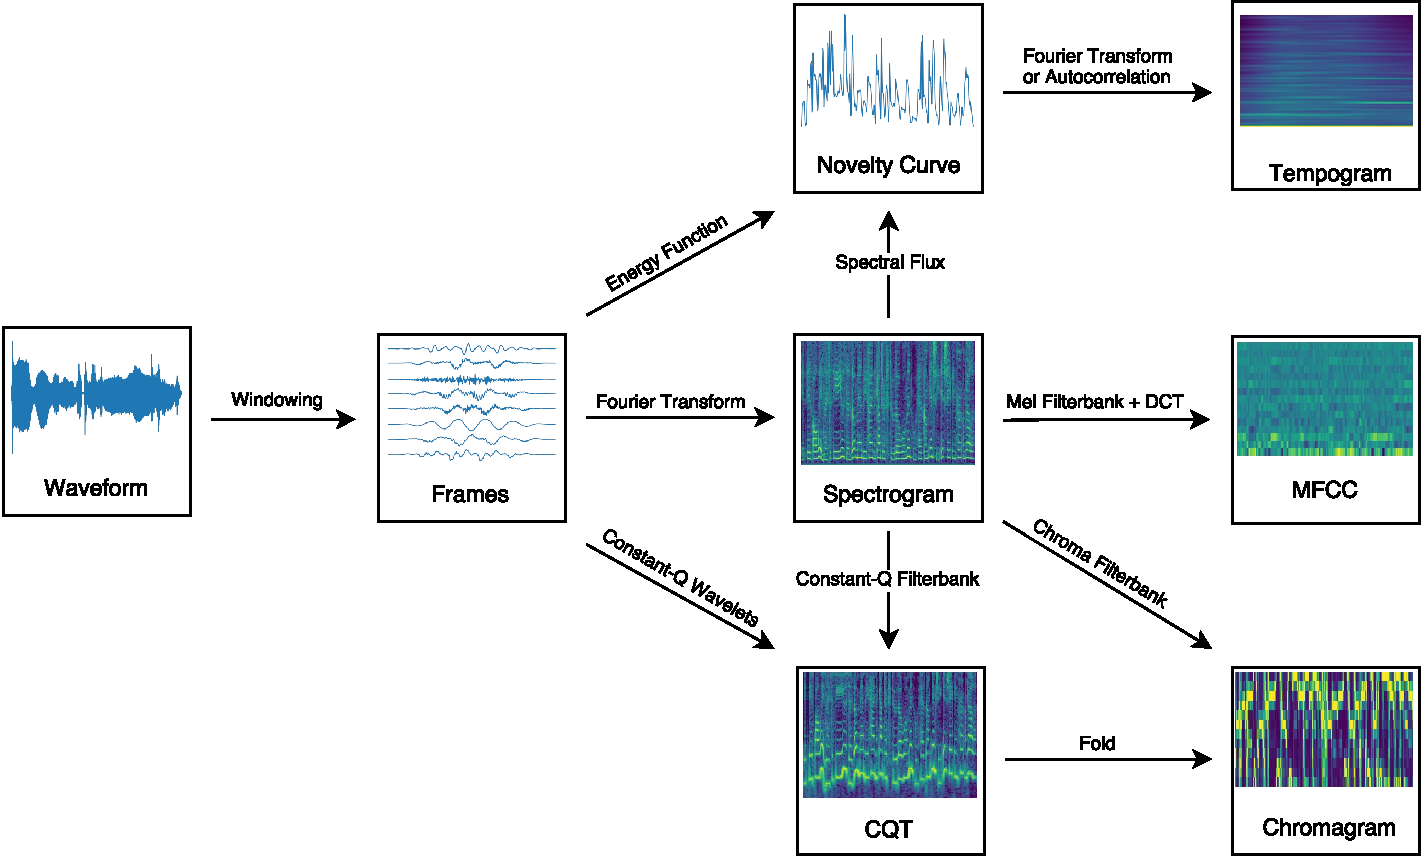
\includegraphics[width=\textwidth]{pipeline.pdf}
	\caption{\small The standard pipeline for music feature extraction. An appropriate set of feature extraction methods needs to be heuristically selected depending on the task.}\label{fig:pipeline}
\end{figure}

This necessitated further transformations by the means of filterbanks, such as \emph{Mel-Frequency Cepstral Coefficients} (MFCC) \cite{logan2000mfcc} by applying the Mel filterbank inspired by the human auditory perception and taking the first few DCT components that contain independent factors describing the spectral shape.
\emph{Constant-Q transform} (CQT) \cite{schorkhuber2010cqt} uses a filterbank where the center frequencies of filters have a constant Q factor, which is the ratio between the center frequency and the 3 dB bandwidth of a filter.
By configuring CQT to produce 12 filters per octave, it is possible to obtain the coefficients corresponding to each musical tone, and to fold the representation to produce a \emph{chromagram} \cite{harte2005chromagram}.
Tonnetz \cite{harte2006tonnetz} is a 6-dimensional feature space signifying harmonic relationships, and more sophisticated feature extractors include the summary ACF \cite{tolonen2000multipitch}, Specmurt \cite{saito2008specmurt}, and bispectrums \cite{argenti2011bispectral}.


To extract the beat and tempo information, a heuristic function, such as the first-order difference of the time-domain log energy function or the \emph{spectral flux} that measures the total energy increase over the STFT frequency bins, is applied to formulate a novelty curve.
This curve can then be used to measure energy bursts that are typically present in the onsets of notes \cite{bello2005onset}.
The onset information can be further processed to obtain tempo information via \emph{tempogram} \cite{cemgil2000tempogram} or cyclic tempogram \cite{grosche2010tempogram}.

Meanwhile, many recent approaches have successfully eliminated some or all feature transformation stages in the standard MIR pipeline by training a deep model directly on spectrograms or audio waveforms.
Applications of deep learning arose in virtually all types of MIR tasks, including melody extraction \cite{bittner2017deepsalience}, beat tracking \cite{vogl2017drum}, and genre classification \cite{oramas2017genre}, and outperformed previous feature-based approaches.
Apart from a small number of end-to-end approaches, most deep learning models for music still rely on predefined feature transforms such as STFT or CQT, because those features leverage the prior knowledge that music signals are often harmonically sparse and make it easier for a model to learn meaningful concepts without overfitting, using a smaller number of parameters and hence being achievable in a limited hardware capacity.
However, any feature extraction stage induces a loss of information, and the best-performing model would benefit most from the raw audio data, given enough amount of training data and hardware \cite{pons2018tagging}.


As is the case for feature extraction, musical prior knowledge is often applied to the algorithmic design of models as well, such as the assumption that sudden changes in music is rare and most changes happen gradually.
In the time domain, median filtering \cite{oudre2009chord} is a simple heuristic that can suppress spurious changes, and \textit{Hidden Markov models (HMM)} are widely employed for modeling sequence data such as chord progressions \cite{cho2010chord} as well as to smooth sequence outputs as a post-processing step \cite{khadkevich2009hmm}.
Prior knowledge about musical notes can be incorporated more specifically. These approaches include detecting onsets and offsets for note transcription \cite{benetos2011polyphonic}, modeling note attacks and decays \cite{cheng2016attackdecay}, and more generally the temporal evolution of notes \cite{cogliati2015temporal}.
In the frequency domain, the \textit{spectral smoothness principle} states that the spectral envelopes of real sounds tend to be slowly varying as a function of frequency \cite{klapuri2003multiple}.
The principle has been implemented in a number of ways, such as a moving-average filter for iterative source estimation and separation \cite{klapuri2003multiple}, a score function for F0 candidate \cite{yeh2010mffe}, and a low-order autoregressive overtone modeling \cite{emiya2010smoothness}.

We have reviewed the common feature extraction stages and identified how the musicological or mathematical prior knowledge on music data guides the algorithmic design of MIR models.
In the following sections, more in-depth literature reviews on the different subtasks relevant to automatic music transcription are provided, starting from the simplest problem of monophonic picth tracking.


\section{Monophonic Pitch Estimation}\label{sec:monophonic}

Monophonic pitch estimation, or pitch tracking, refers to the task of extracting the fundamental frequency (F0) values from monophonic audio signals.
Formally, pitch is defined as a subjective quality of perceived sounds and does not precisely correspond to the physical property of the fundamental frequency \cite{hartmann1997signals}.
However, apart from a few rare exceptions, pitch can be quantified using fundamental frequency, and thus they are often used interchangeably in the MIR literature outside psychoacoustical studies. 
Since differentiating the physical and the perceptual aspects of pitch is a non-goal, the two terms are interchangeably throughout this thesis as well.

Computational methods for monotonic pitch estimation have been studied for more than a half-century \cite{noll1967cepstrum}, and many reliable methods have been proposed since.
Earlier methods commonly employ a certain candidate-generating function, accompanied by pre- and post-processing stages to produce the pitch curve.
Those functions include the cepstrum \cite{noll1967cepstrum}, the autocorrelation function (ACF) \cite{dubnowski1976acf}, the average magnitude difference function (AMDF) \cite{ross1974amdf}, the normalized cross-correlation function (NCCF) as proposed by RAPT \cite{talkin1995rapt} and PRAAT \cite{boersma1993praat}, and the cumulative mean normalized difference function as proposed by YIN \cite{decheveigne2002yin}. More recent approaches include SWIPE \cite{camacho2008swipe}, which performs template matching with the spectrum of a sawtooth waveform, and 
pYIN \cite{mauch2014pyin}, a probabilistic variant of YIN that uses a Hidden Markov Model (HMM) to decode the most probable sequence of pitch values.
According to a few comparative studies, the state of the art is achieved by YIN-based methods \cite{von2010comparison, babacan2013comparative}, with pYIN being the best performing method to date.

Since the methods for monophonic pitch tracking are usually built based on the assumption that at most one pitch is present at a time, they cannot be directly applied to polyphonic music where multiple concurrent notes and sound sources are present.
Different approaches are therefore needed to accurately estimate multiple concurrent pitches, and such methods are reviewed in the next section.


\section{Multiple Fundamental Frequency Estimation}\label{sec:mffe}

Among the subtasks of automatic music transcription, estimating and tracking all pitches from a polyphonic recording poses the most difficult challenges, as apparent from the recent stream of results from MIREX challenges \cite{downie2014mirex}.
The task is commonly referred to as \emph{multiple fundamental frequency estimation} (Multi-F0 estimation, or MFFE) or \emph{multi-pitch estimation} (MPE).
This task is in some sense a superset of other MIR tasks like onset detection, beat tracking, chord recognition, and melody extraction,
since the frequency tracking task has to indicate the presence of every pitch, and tracking chords and melodies becomes much easier when the correct annotations for all pitch values are available.


%%% Early approachs including blackboard systems

Early approaches for polyphonic pitch tracking are often based on rather strict assumptions on the types of timbre and the number of polyphony in the audio to be transcribed \cite{moorer1977transcription,piszczalski1977transcription}. Blackboard systems \cite{martin1996blackboard,dixon2000piano} are one of the first methods that enabled polyphonic transcription to work under milder assumptions, by integrating both signal processing and musicological knowledge into hierarchical problem abstraction. Limitations of the blackboard approach include the overall complexity and the exhaustive searches required by the system. Accordingly, later approaches often use statistical models or factorization-based methods to more efficiently capture pitch information.


%%% NMF and its variants

\textit{Non-negative matrix factorization (NMF)} \cite{lee1999nmf,lee2001nmf} refers to an algorithm that finds two matrices that factorize a given matrix where the elements of all three matrices are non-negative.
Starting with \citeA{smaragdis2003nmf}, many successful methods for music transcription have been built based on NMF \cite{benetos2019amt}.
These methods commonly take the approach of factorizing a time-frequency representation $\X \in \R^{F \times T}$ as a product of a dictionary matrix $\mathbf{D} \in \R^{F \times K}$ and an activation matrix $\mathbf{A} \in \R^{K \times T}$, where $K$ is the number of pitch labels to be transcribed, e.g. 88 keys for piano transcription.
This allows for an intuitive interpretation of each matrix, where each column of $\mathbf{D}$ contains a spectral template for a pitch label, and each row of $\mathbf{A}$ contains the activation of the corresponding pitch over time.
Various extensions of factorization-based methods have been proposed to leverage sparsity~\cite{abdallah2004sparse,cont2006realtime,costantini2013nmf}, non-negative matrix division \cite{niedermayer2008division}, $\beta$-divergence \cite{dessein2010beta}, adaptive estimation of harmonic spectra~\cite{vincent2010adaptive,fuentes2013harmonic}, a Bayesian framework for encouraging harmonicity and temporal smoothness \cite{bertin2009nmf,bertin2010nmf,peeling2010factorization}, and modeling of attack and decay sounds~\cite{benetos2013multi,ewert2016admm}.
With carefully designed regularizers and the \textit{alternating direction method of multipliers (ADMM)} for training NMF, \citeA{ewert2016admm,ewert2017admm} achieved close-to-perfect accuracy for piano transcription in a studio setting, i.e. when the exact spectral profile of the piano notes to be transcribed is known in advance.

  

%%% PLSA (aka PLSI or PLCA)

A probabilistic approach closely related to NMF is \textit{probabilistic latent semantic analysis (PLSA)} \cite{hofmann1999plsa}, a simple probabilistic graphical model that factorizes the joint probability distribution of time and frequency into conditional distributions involving a latent semantic factor.
PLSA is is equivalent to NMF when the KL divergence is minimized under $L_1$ normalization \cite{gaussier2005plsa,ding2008equiv}, while the probabilistic framework enables statistical learning and introducing transformation invariances \cite{smaragdis2006latent}.
In \cite{smaragdis2009relative,benetos2012latent}, a shift-invariant extension to PLSA has been applied to multi-instrument MFFE by using a convolution over constant-Q spectrograms.
\citeA{grindlay2010subspace} proposed an extension to PLSA based on the \textit{subspace NMF} algorithm \cite{grindlay2009eigeninstruments} for multi-instrument MFFE, incorporating additional parameters for instrument sources and possible pitch values.


%%% Bridging to general (Bayesian) probabilistic methods

Many probabilistic models for music transcription employ a Bayesian framework, in which the audio signal is modeled using a probability distribution conditional on unobserved variables such as the note frequencies and timing.
The transcription is then performed through Bayesian inference on those parameters, using either \textit{Markov-chain Monte Carlo (MCMC)} or \textit{variational inference}.
Bayesian models for music transcription are usually designed with prior and conditional distributions incorporating musicological and acoustical knowledge on the music and the instruments to be transcribed, such as the de-tuning of partials \cite{davy2003harmonic}.
Existing approaches in directions include
a state-space model for musical harmonics \cite{cemgil2003generative},
a decomposition of audio signals into Gabor atoms \cite{davy2006bayesian}, 
a hierarchical graphical model \cite{pesek2017hierarchical},
and an overtone corpus encoding the harmonic structure \cite{sakaue2013overtone}.
A nonparametric Bayesian model proposed in \cite{yoshii2012nonparametric} employs infinite Gaussian mixtures and noninformative hyperprior distributions, automating the model selection process.
Bayesian models provide a powerful tool connecting the whole generative process of music, but usually suffer from the high computational cost and the complexity of the algorithm.


%%% Simple data-driven classification models

Unlike the aforementioned approaches which incorporate as much prior knowledge on the music as possible, discriminative models employ a simpler approach of learning a direct mapping between the audio features and the labels from large training data, making minimal assumptions on the acoustical or musical structure.
This data-driven approach is made possible by the availability of large datasets and increased computational capabilities.
\textit{Support vector machines (SVM)} were commonly used in earlier discriminative approaches, by constructing one-versus-all SVM classifiers on STFT magnitudes \cite{poliner2006discriminative}, on learned features using \textit{deep belief networks (DBN)} \cite{nam2011classification}, or on the result of NMF \cite{weninger2013nmf}.
While being flexible and straightforward to be applied on any features of choice, SVMs have high time and space complexities which limit the size of training dataset and hence the capability of the model.


%%% Neural networks and deep learning


Deep learning~\cite{lecun2015deeplearning} methods for music transcription are increasingly popular~\cite{benetos2019amt}, as larger labeled datasets and more powerful hardware become accessible.
These approaches commonly employ \textit{neural networks (NN)} to produce music transcriptions from the input audio representation, and these are relatively recent phenomena that started in the last decade, with a notable exception of \citeA{marolt1999nn,marolt2004connectionist}.
\citeA{nam2011classification} used deep belief networks~\cite{hinton2006dbn} to extract audio features which are subsequently fed to pitch-wise SVM-HMM pairs to predict the target piano rolls.
More recent approaches are based on \textit{convolutional neural networks (CNN)} and/or \textit{recurrent neural networks (RNN)}.
Transcription models using CNNs are relatively simpler to train and deploy since they can be easily applied in a frame-wise manner in parallel, and they are shown effective especially for the cases where the notes mostly contain sustained sounds, such as bowed strings, wind instruments, and vocals~\cite{kelz2016framewise,bittner2017deepsalience}.
The sequential nature of RNNs is suitable for modeling the temporal variations in music, and many neural transcription models include recurrent connections in their architecture.
RNN architectures proposed for AMT include bidirectional RNNs \cite{bock2012rnn}, recurrent temporal \text{restricted Boltzmann machines} \cite{boulangerlewandowski2012temporal}, an acoustic model combined with an RNN-based music language model \cite{sigtia2015hybrid,sigtia2016endtoend,wang2018mlm},
a sequence-to-sequence model \cite{ullrich2017seq2seq},
a dual-objective loss for onsets and frames \cite{hawthorne2018onsetsframes},
and a \textit{convolutional-recurrent neural networks (CRNN)} \cite{thome2017crnn}, which scored the top accuracy in the MFFE subtask of the MIREX 2017 competition.


%%% 

A few recent studies tried to identify the limitations of simply improving the conventional metrics and argued the need for more systematic analysis and assessment of the music transcription problem.
These include a study of invariances under data augmentation \cite{thickstun2018invariances}, a study of the entanglement of note representations that may prevent accurate predictions for unseen combinations of notes \cite{kelz2017entanglement}, and a musically inspired evaluation metric that also takes account of voice separation and harmonic analysis \cite{mcleod2018eval}.



\section{Source Separation and Music Translation}\label{sec:separation}

Source separation refers to the task of separating sound sources from a mixture signal, and is closely related to automatic music transcription, because it provides a means to separate each instrument sources from multi-instrument music.
This problem is also called as a \emph{cocktail party problem}, based on humans' ability to focus on a single voice at a noisy cocktail party.
Sound source separation has been a popular research topic since the seminal work on \emph{auditory scene analysis} by \citeA{bregman1990asa}, from which stemmed computational auditory scene analaysis (CASA) \cite{brown1994casa}, a problem of using computational models to analyze an auditory scene, identifying the sources and location of all nearby sounds.
In this sense, automatic music transcription and sound source separation are particular aspects of auditory scene analysis \cite{plumbley2002transcription}, and source separation enables similar kinds of applications to AMT, such as music editing, 3D sound rendering, and information retrieval systems.


\emph{Blind source separation} refers to the situation where no information about the sources or the mixing process is known \cite{bell1995blind}, whereas \emph{informed source separation} \cite{vincent2013separation} concerns the case where some level of side information is available, e.g. the presence of a score \cite{ewert2014separation}.
Blind sound source separation has to resort to using purely statistical approaches such as indepenent component analysis \cite{saruwatari2006ica} or robust PCA \cite{huang2012separation}, whereas informed source separation can leverage the knowledge on the musical structure \cite{rafii2013separation, liutkus2012separation} or the timbral differences of the sources \cite{li2007separation,ono2010hpss} for better separation.
Probabilistic models for source separation \cite{ozerov2007separation,leglaive2016prior} have also been developed, and source-filter modeling \cite{heittola2009separation,durrieu2011separation} is a generative approach which separately models a source that creates a sound and a filter that shapes the timbre.
The proposed AMT model is similar to source-filter models in a sense that it describes the generative process of each sound, but also relates to timbre-informed source separation models \cite{miron2018thesis}, because it needs to learn the concept of timbre to produce per-instrument piano rolls.


A closely related problem to source separation is audio translation, which concerns mapping input audio to a corresponding output with some desired properties, such as speech with reduced noise, singing voice separated from music, or the same speech content in the voice of a different speaker.
\citeA{barry2018style} applied the style transfer algorithm \cite{gatys2015style} to an ensemble of STFT, CQT, and Mel spectrograms, to transfer musical styles capturing harmonic, rhythmic, and timbral elements.
The \emph{U-Net} architecture \cite{ronneberger2015unet} uses an encoder-decoder framework with skip connections between the hidden layers at the same level of abstraction to perform image translation, and a singing voice separation model can be trained using this architecture \cite{jansson2017separation}.
The encoder-decoder architecture with skip connections can also be trained with GAN objectives, and a few audio translation models working on spectrograms have been developed; examples include singing voice separation \cite{fan2017svsgan, stoller2017separation}, source separation \cite{subakan2017gan}, and speech enhancement \cite{pascual2017segan, donahue2017segan}.



\section{Machine Learning Models for Music Synthesis}

The recent deep generative have been very successful in synthesizing breathtakingly high-quality audio signals.
We would want the synthesized music and audio signals to capture the long-term dependencies such as beats, measures, and chord progressions that ranges up to a few seconds, while the raw audio signals typically have the order of 10 thousand sameples per second.
This made end-to-end synthesis models more difficult to train than image synthesis and translation models which it usually suffices to capture dependencies ranging a few hundred pixels.
SampleRNN \cite{mehri2016samplernn}, to be discussed in Chapter \ref{ch:deeplearning} in the context of deep autoregressive models, is one of the first successful deep generative models for audio and formed a basis for the techniques used by Lyrebird, an AI startup founded by University of Montr\'{e}al students that provides API for synthesized voice of a specific person, e.g. Barack Obama.
WaveNet \cite{oord2016wavenet}, developed by Google DeepMind, uses a causal architecture using dilated convolutions to generate time-domain audio samples, and is able to produce realistic human voices and piano sounds.
WaveNet learns acoustically meaningful representations including pitch and spectral features \cite{hua2018wavenet}.
There also exist faster approaches using recurrent neural networks to produce vocal and musical audio, as found in \cite{nayebi2015gruv} and \cite{kalingeri2016generation}, albeit with lower quality when compared to WaveNet.
Tacotron \cite{wang2017tacotron, shen2018tacotron} is a fully end-to-end speech synthesizer that works directly on a sequence of characters, which can learn the pronunciation of unseen complex words and different ways of reading the same word according to the phrase semantics and punctuations.
A newer RNN-based model called WaveRNN \cite{kalchbrenner2018wavernn} is capable of generating audio that matches WaveNet in quality, yet with an enough efficiency to be able to run real-time on GPUs or even on mobile phones.
WaveGlow~\cite{prenger2019waveglow} uses a flow-based approach to synthesize waveform samples and is also shown to produce WaveNet-quality audio while being able to run efficiently in parallel.
A singing synthesis model \cite{blaauw2017singing} based on the WaveNet architecture is also capable of synthesizing voice parametrically, separating the influence of pitch and timbre in the model.
% A music synthesis technique employing a similar approach as the above will be a key component of the overall architecture, allowing the transcription model to generate realistic-sounding music to compare with the input audio.

\textit{Generative Adversarial Networks (GANs)}, also to be reviewed extensively in Chapter \ref{ch:deeplearning}, have also been used as generative models for audio.
A GAN architecture using one-dimensional convolutions called \emph{WaveGAN} was introduced by \citeA{donahue2018wavegan} and is capable of generating 1-second audio segments from the latent representations.
In a newer approach called \emph{GANSynth}~\cite{engel2019gansynth}, the GAN architecture was used for generating magnitude spectrograms together with the corresponding two-dimensional representation of instantaneous frequencies, which produced significantly more stable output compared to WaveGAN.
Training GANs for arbitrary-length audio sequences and extending it as a tool for disentanglement of latent semantic information or a conditional audio synthesis framework remains a challenge.

\section{Music Language Models for Symbolic Music Generation}

Symbolic music processing refers to the techniques for processing music at a symbolic level, such as in the form of sheet music, MIDI signals, or piano roll representations.
Problems in this domain include optical music recognition \cite{rebelo2012omr}, algorithmic composition \cite{fernandez2013ai}, and computational music theory \cite{hamanaka2013computational}, while the subject most relevant to music transcription research would be \emph{music language models}.
A music language model is a statistical model, often a generative model, that encodes music theoretic knowledge to describe the structural composition and arrangement of musical elements \cite{patel2010musiclanguage}, similarly to how computational linguists build language models to describe the structure of natural languages.
A well-designed music language model can be an important component for a generative model for music, because it can serve as a prior for latent representations and can be combined with conditional synthesis models or software instruments to produce audio.
% As a side note, there are two distinct objectives for symbolic music generation systems --- style imitation and genuine composition \cite{nierhaus2009composition} --- among with this thesis only focuses on the former, aiming at informing the transcription model about music theoretic knowledge rather than imagining a new type of musical art.

The first systematic approach of applying a linguistic theory to music was the \emph{generative theory of tonal music} \cite{lerdahl1983gttm}, which was inspired by Noam Chomsky's generative grammar \cite{chomsky1966generative} and was influential in music theory, music psychology, and cognitive musicology.
Music language models implement this idea using computational methods, typically involving statistical models that are also used in natural language processing.
These include many kinds of approaches for symbolic music generation, such as hidden Markov models \cite{farbood2001markov}, generative grammars \cite{chemilier2001grammar}, cellular automata \cite{burraston2004automata}, and genetic algorithms \cite{miranda2007evolutionary}.
More recently, deep learning models such as recurrent neural networks have been used to build music language models \cite{sigtia2014lm}.
The latest approaches to generate realistic music sequences in the symbolic domain include an application of variational autoencoder \cite{teng2017generating,tikhonov2017generation}, a generative adversarial network \cite{yang2017midinet}, and a transformer~\cite{huang2019transformer}.

\section{Summary}

In this chapter, a broad range of MIR techniques related to automatic music transcription have been discussed, in the fields of monophonic and polyphonic pitch tracking, source separation and music translation, music synthesis, and music language models.
A clear observation in each subtask of AMT is that many recent methods employ deep learning models, and this is because deep models have more flexibility and capacity to learn complex statistical relations of interest.
In order to build the solid foundation of the various deep learning techniques used throughout this thesis, Chapter \ref{ch:deeplearning} will provide an extensive review on the various techniques and models that are collectively classified as deep learning.

%!TEX root = ../dissertation.tex
% this file is called up by thesis.tex
% content in this file will be fed into the main document

\graphicspath{{3-deeplearning/figures/}}

\chapter{Deep Learning and Deep Generative Models}\label{sec:deeplearning}
\label{ch:deeplearning}

Since recently, a family of machine learning research under the term \emph{deep learning} has incurred many groundbreaking changes to the world of artificial intelligence, making the long-waited dream of the \emph{artificial general intelligence} (AGI) \footnote{a loosely defined term referring to human-level intelligence, i.e. an AI system that can solve complex problems in varied and possibly previously-unseen domains with self-understanding and autonomous self-control. \cite{goertzel2007agi}} look not so distant in the future.
The impact of deep learning has been so dramatic that many successful applications of deep learning like DeepMind's AlphaGo outplaying the human Go champion and Google's neural machine translation have became familiar to the general public.
The core idea of using artificial neural networks to process complex information traces back to the earliest days of computing \cite{kleene1951representation} but has long been considered less effective than alternative methods, such as support vector machines or probabilistic graphical models.
Since around 2010, it has been increasingly shown that neural networks can substantially outperform those other approaches and have much more capability for further improvements, and that the lower performance of neural networks in the past was merely due to insufficient data, the lack of computational power, and some numerical tricks that had not been employed before.
This finding has opened the era of deep learning --- a term coined after the fact that neural networks often employ multiple layers of learned feature transformations --- and is continuing to innovate virtually all fields of science and engineering, including, of course, music technology.

This chapter reviews the essential concepts and terminologies of deep learning, from the basic architectures and techniques to the most recent advances in deep generative models.
The purpose of this chapter is to present a historical perspective toward deep generative models and to provide a motivation for building music transcription systems upon them in the proposed research.


\section{Neural Network Architectures}

The key idea of an artificial neural network in the simplest setting is to find an appropriate matrix $W$ to model the relationship between variables $\bm{x}$ and $\bm{y}$, so that
\begin{equation}\label{eqn:perceptron}
	\bm{y} = \sigma(W \bm{x})
\end{equation}
is a good approximation, where $\sigma$ is a nonlinear function like the sigmoid or the hyperbolic tangent.
This model in Equation \ref{eqn:perceptron} is also known as a \emph{perceptron} \cite{rosenblatt1957perceptron}, one of the first artificial neural networks in history.
This computation --- a matrix multiplication followed by a nonlinear activation --- can be applied multiple times, like
\begin{equation}\label{eqn:mlp}
	\bm{y} = \sigma(W_3\sigma(W_2 \sigma(W_1 \bm{x}))),
\end{equation}
which gives the model more expressive power, meaning that it can learn more complex relationship in the data that the previous model could not discern, e.g. the XOR problem \cite{riedmiller1994mlp}.
The model in Equation \ref{eqn:mlp} is called a \emph{multilayer perceptron} (MLP) in a sense that it is a concatenation of perceptrons, and the fact that it contains multiple layers is why these neural networks are called ``deep".


A multilayer perceptron is a special case of feedforward neural networks, which refer to any computational graph that does not contain a cycle.
A popular model under this category is \emph{convolutional neural networks} (CNN), which uses a convolution (a cross-correlation, to be precise) with fixed-size kernels instead of matrix multiplications.
A 2-D convolutional layer takes input arrays $X_c \in \mathbb{R}^{H \times W}$, $c \in \{ 1, \cdots, C \}$, and produces output arrays $Y_d \in \mathbb{R}^{H \times W}$, $d \in \{ 1, \cdots, D \}$.
The kernels $K_{cd} \in \mathbb{R}^{K_1 \times K_2}$, $c \in \{ 1, \cdots, C \}$, $d \in \{ 1, \cdots, D \}$, and the biases $\bm{b} \in \mathbb{R}^D$ are the parameters to be optimized, and the output is calculated as:
\begin{equation}\label{eqn:convnet}
Y_{d}[i,~j] = \sum_{m=1}^{K_1} \sum_{n=1}^{K_2} \sum_{c=1}^C K_{cd}[m,~n] X_c[i+m,~j+n] + b_d
\end{equation}
There are various options to this operation including whether to pad the input or trim the output of the convolution to according to the kernel size, and how much to stride the kernels while moving along the input arrays.
The 2-D convolution is suitable for image data, where the initial $C$ can be the 3 RGB channels of color images, while the similarly-defined 1-D and 3-D convolutions are more often used with time-series and video data respectively.

Using convolutional layers results in a fewer number of parameters to learn in each layer than the equivalent multilayer perceptron, allowing deeper models for the same total number of parameters.
LeNet \cite{lecun1995lenet} for digit classification is what pioneered the technique of using convolutional layers in neural networks, which has become an essential building block of the majority of deep learning methods.
Such models include those that surpassed the human-level accuracy in the ImageNet Large Scale Visual Recognition Challenge (ILSVRC) \cite{krizhevsky2012imagenet, simonyan2014vgg, szegedy2015googlenet, he2016resnet}.
A standard practice of building a CNN is to stack a multiple convolutional layers along with pooling layers to obtain a compact feature repesentation, which is fed to a multi-layer perceptron as in Equation \ref{eqn:mlp} to produce output.
The layers of MLP are called fully connected or dense layers, because unlike the convolutional layers, the weight matrix used in the matrix multiplication associates every pair of the input and output features.
\emph{Fully convolutional networks}, which omit the fully connected layers that are typically placed at the last stages of neural networks, do not require a fixed input and output size and are known to perform well for image segmentation \cite{shelhamer2017fcn}.
Using the ability of deep convolutional layers to extract complex semantic information from images, many artistic applications have been developed, such as the transfer of artistic style from one image to another \cite{gatys2015style}, and a captivating transformation of images using neural network weights known as \emph{Deep Dream} \cite{mahendran2016deepdream}.


A network with cyclic connections is called a \emph{recurrent neural network} (RNN), and has been successfully applied to modeling sequential data.
Because it is hard for a recurrent neural network to propagate long-range dependencies through a chain of recurrent connections, specific recurrent units called long short-term memory (LSTM) \cite{hochreiter1997lstm} and gated recurrent unit (GRU) \cite{cho2014seq2seq} are devised to resolve the problem and are considered essential for recurrent neural networks.
A formulation of recurrent neural network called the sequence-to-sequence model \cite{cho2014seq2seq,sutskever2014seq2seq}, which can model a mapping from variable-length input to variable-length output, is well known to be very effective for machine translation, and is deployed in production in Google's translation services \cite{wu2016google}.
An important technique for building recurrent neural networks is \emph{attention} \cite{bahdanau2014attention}, which allows the network to focus on specific parts of a sequence for generating outputs.
The attention mechanism is shown to be effective in tasks including not only machine translation as in the original paper, but also in image description generation \cite{karpathy2017desc}, speech recognition \cite{chorowski2015speech}, and question answering \cite{sukhbaatar2015memory}.

\emph{Reinforcement learning} is a formulation of machine learning where a software agent takes actions in an environment to maximize the reward given according to the actions \cite{sutton2018reinforcement}.
This formulation is inspired by behaviorist psychology and is well-suited for environments that require explorations by the agent, such as robotics and games.
Deep Q-Network (DQN) \cite{mnih2015dqn} is a neural network model designed for reinforcement learning, which has been successfully applied to automatically playing Atari games \cite{mnih2013atari} and the agent playing the game of Go that surpassed the human level of skill \cite{silver2016alphago}.


\section{Performance Optimization Techniques}

The success of deep learning was possible not only because of the architectural design of deeper models and the hardware capable of supporting such models, but also due to the numerous elaborate techniques and clever tricks that enabled previously impossible performances.

Training a neural network involves optimization of its parameters, e.g. the weights $W$ in Equation \ref{eqn:perceptron}-\ref{eqn:mlp} and the kernels $K_{cd}$ in Equation \ref{eqn:convnet}, which typically requires the gradient of the loss function, i.e. the partial derivatives with respect to all of the model's parameters.
It is feasible to manually derive the gradient for simple models, but for deep neural networks it is often too complex and error-prone to calculate the derivative by hand.
For this reason, a method called backpropagation \cite{werbos1982backpropagation, rumelhart1986backpropagation} was introduced based on the ideas of automatic differentiation \cite{linnainmaa1970ad} and revived neural network research that had been largely abandoned.
The popularization of \emph{backpropagation} in the 1980s partly contributed to the ending of the first AI winter, leading to the first commercially successful application of neural network in optical digit recognition and speech recognition.
Backpropagation is still a fundamental element of deep learning, and many deep learning frameworks are capable of automatically calculating gradients using backpropagation when a compute graph is given.
This enables the developer to write only the forward calculation and run the backpropagation automatically, greatly improving the productivity.


Once a gradient is known, the standard way of optimizing a neural network is to use a variant of \emph{stochastic gradient descent} (SGD), where the direction of the gradient descent is determined only based on a mini-batch of training data.
Although using only a tiny subset of training data makes the gradient unstable, in practice, stochastic gradient descent converges faster than batch gradient descent using the same amount of training samples.
Adding momentum in the gradient descent optimizer has shown to be effective for finding the convergence even faster, and many schemes for applying the momentum have been introduced, such as Adagrad \cite{duchi2011adagrad}, RMSprop \cite{hinton2012rmsprop}, Adadelta \cite{zeiler2012adadelta}, and Adam \cite{kingma2015adam}.
While Adam is by far the most popular choice of optimizer, a few modification to Adam's algorithm have been proposed, including Eve \cite{koushik2016eve} using feedback from the objective function, Nadam \cite{dozat2016nadam} incorporating Nesterov's accelerated gradient descent, and AMSgrad \cite{reddi2018amsgrad} fixing a failure case of Adam where it does not converge to the optimum even in a simple convex optimization problem.

Historically, the sigmoid and the hyperbolic tangent function have been popular choices for the nonlinearity, but it is surprisingly shown \cite{nair2010relu} that the \emph{rectified linear units} (ReLU),
\begin{equation}
	f(x) = \max \{ x, 0 \},
\end{equation}
generally improves the accuracy of deep learning models.
It is also known that neural networks with ReLU activations converge faster, and more robust to the vanishing gradient problem.
A number of ReLU variants, including leaky ReLU \cite{xu2015leakyrelu}, parametric ReLU (PReLU) \cite{he2015prelu}, SReLU \cite{jin2015srelu}, have been devised and shown to be effective in some cases.


As with any other machine learning methods, overfitting is a problem to overcome for deep learning models as well.
While directly adding a L1 or L2 regularization term of weights is possible, a few cleverer tricks for preventing overfitting have been devised and widely employed, and they are treated as regularization methods in a wider sense.
\emph{Dropout} \cite{srivastava2014dropout} is a simple yet powerful regularization method that turns off a random subset of activations during the training process.
Because the network has to learn how to make accurate predictions using only a random subset of its components, the training becomes more robust and less susceptible to overfitting.
\emph{Batch normalization} \cite{ioffe2015batchnorm} is a method to reduce what the covariance shift of activations, by performing normalization for each training mini-batch so that the activations of each layer have zero mean and unit variance.
It has also been empirically shown to improve the generalizability of the trained model.
Despite being relatively new, dropout and batch normalization are drop-in methods that can be added to most deep architectures with almost no changes to code and yet significantly improve the performance and are thus included almost by default in the majority of newer deep models.
\emph{Scaled exponential linear units} (SELU) \cite{klambauer2017selu} use a special activation function that induces a self-normalizing property over layers, making the activations have zero mean and unit variance without using batch normalization explicitly.


Additionally, because typical neural networks contain thousands to millions of parameters to train, a proper initialization of the weights prior to training is important.
In early days of deep learning, unsupervised pre-training of weights \cite{bengio2007greedy,erhan2010pretraining} was considered necessary, but recently it is shown that a simple random initialization of weights is sufficient with the current computational power of the hardware.
A widely practiced way of initializing the weights without unsupervised pre-training is to sample from a Gaussian or uniform distribution, scaled according to the number of input and output nodes \cite{glorot2010initialization,he2015prelu}.


\section{Toward Deep Generative Models}

Statistical models that describe how data is generated are called \emph{generative models} and provide means of generating samples of data, either by directly modeling the data distribution or through a sampling procedure specified by the model which implicitly defines the probability distribution.
This is in contrast with \emph{discriminative models}, which can only predict the labels corresponding to the given data samples.

\subsection{Traditional Models}

Classic examples of generative models include \emph{na\"{i}ve Bayes classifiers} \cite{maron1961naive} which model a conditional distribution of each feature assuming they are conditionally independent given the label and use Bayes' theorem to predict the labels.
\emph{Gaussian mixture models} (GMM) \cite{everitt1981mixture} approximates the data distribution with a mixture of multivariate gaussian distributions.

While these simple models work effectively to a certain degree with a well-crafted set of features, it is desirable to have generative models that can capture more intricate geometry of the data distribution.
\emph{Probabilistic graphical models} (PGM) specify the structural dependencies between random variables using graphs, with nodes representing random variables and connections between them representing their dependencies.
The graphs can have directed or undirected connections to formulate the joint probability distributions of the variables.
\emph{Hidden Markov models} (HMM) \cite{rabiner1989hmm} and \emph{latent Dirichlet allocation} (LDA) \cite{blei2003lda} are special cases of directed probabilistic graphical models, also called \emph{Bayesian networks}, and are widely used for sequence modeling and topic modeling, respectively.
Undirected graphical models, also called \emph{Markov random fields} (MRF), have many applications in image processing, typically by having connections between nodes corresponding to adjacent pixels.
Undirected graphical models where every pair of nodes has a connection are called \emph{Boltzmann machines} and are capable of learning internal representations of data.

\subsection{Early Deep Generative Models and Autoregressive Models}

\emph{Restricted Boltzmann machines} (RBM) are simplified variants of Boltzmann machines consisting of two layers of nodes with only interlayer connections, and unlike Boltzmann machines, there exists a relatively efficient algorithm \cite{hinton2005cd} for training restricted Boltzmann machines.
\emph{Deep belief networks} (DBN) \cite{hinton2006dbn} are composed of multiple layers of restricted Boltzmann machines, which can be trained using greedy layer-wise optimization, and are capable of classifying hand-written digits as well as conditionally generating them.
Although deep belief networks are one of the first successful deep learning applications and gave many architectural and algorithmic insights to the development of deep learning in the subsequent years, the algorithms for training DBNs are not as scalable as those for other discriminative models like stochastic gradient descent, and eventually faded away in favor of the discriminative models that runs more effectively with a larger scale of data.

An alternative method to generate data samples using a neural network is to produce one element (i.e. one audio sample or one pixel) at a time by feeding the previous elements to the network.
This approach is called an autoregressive model, and many architectures based on this idea including NADE \cite{larochelle2011nade}, DARN \cite{gregor2013darn}, RIDE \cite{theis2015ride}, DRAW \cite{gregor2015draw}, PixelCNN/PixelRNN \cite{oord2016pixelrnn}, SampleRNN \cite{mehri2016samplernn}, WaveNet \cite{oord2016wavenet}, and WaveRNN \cite{kalchbrenner2018wavernn} are proposed and shown to be capable of generating image and audio samples.
However, in addition to being inevitably slow having to repetitively run the model for every element, a drawback of autoregressive models is the difficulty of interpreting the representation, because the autoregressive model only encodes the local dependency of one sample on the adjacent elements and does not provide a compact latent representation corresponding to the global structure.

\subsection{Variational Autoencoders}

A straightforward method to obtain a compact latent representation from unlabeled data is to build an encoder that transforms the input data into a smaller latent dimension, followed by a decoder that maps it back to the original data.
This architecture is called an \emph{autoencoder} \cite{bengio2009deeplearning}, and being a deep extension to principal component analysis (PCA), it is capable of learning a nonlinear mapping for dimensionality reduction.
The autoencoder architecture are shown to be effective at encoding the latent representation of data, through a few successful variants including sparse autoencoder \cite{ng2011sparse} which produces a sparse representation of the input data, denoising autoencoder \cite{vincent2008denoising} which is capable of reducing noise or recover a redacted portion of an image, and contractive autoencoder \cite{rifai2011contractive} which adds a regularization term to make the model robust to slight variations of input values.


Autoencoders are not generative models in a strict sense, because, while its decoder part can produce data samples from their latent representations, it lacks the ability to randomly sample the points in the latent dimensions that corresponds to the data distribution.
\emph{Variational autoencoders} (VAE) \cite{kingma2013vae} address this problem by restricting the posterior latent distribution to be Gaussian.
This is achieved by variational inference, reformulating the evidence lower bound (ELBO) of the data log-likelihood as:
\begin{equation}\label{eqn:vae}
\log p(\bm{x}) \ge \mathcal{L}(p_\theta, q_\phi) = \mathbb{E}_{q_\phi(\bm{z}|\bm{x})} [\log p_\theta(\bm{x}|\bm{z})] - \mathrm{KL}(q_\phi(\bm{z}|\bm{x}) || p(\bm{z})),
\end{equation}
where $q_\phi(\bm{z}|\bm{x})$ models the encoder and $p_\theta(\bm{x}|\bm{z})$ models the decoder, and both are parameterized using neural networks which provides a flexible and differentiable family of functions.
Note that maximizing $\mathcal{L}$ will maximize the first term of RHS, the log likelihood of the reconstructed data, and minimize the second term, the KL divergence between the encoded data distribution and the prior, serving as a regularizer that induces the posterior to be Gaussian.
The Gaussian prior gives the KL divergence a closed-form solution making it straightfoward to derive the derivative according to $\phi$, whereas the first term contains an expectation over a distribution depending on $\phi$, which disallows moving the gradient operator into the expectation and makes the stochastic gradient descent and backpropagation impossible.
A reparameterization trick is used to address this issue, by setting $\bm{z} = g({\epsilon}, \bm{x}) = \bm{\mu}_\phi (\bm{x}) + {\epsilon} \cdot \bm{\sigma}_\phi(\bm{x})$ where $\epsilon \sim \mathcal{N}(0, 1)$, which gives:
\begin{equation}\label{eqn:reparam}
\nabla_\phi \mathbb{E}_{q_\phi(\bm{z}|\bm{x})} [\log p_\theta(\bm{x}|\bm{z})] = \nabla_\phi \mathbb{E}_{\epsilon} [\log p_\theta(\bm{x}|g(\epsilon, \bm{x}))] = 
\mathbb{E}_{\epsilon} [\nabla_\phi \log p_\theta(\bm{x}|g(\epsilon, \bm{x}))],
\end{equation}
making the stochastic gradient ascent and backpropagation on the ELBO possible.


The biggest drawback of variational autoencoders, however, is the blurriness in reconstructed images, that may come from the inexactness of the Gaussian assumption and the variational lower bound used by the model \cite{doersch2016tutorial}.
There have been many attempts to overcome this by allowing more flexible prior distributions \cite{rezende2015flow} as well as better latent representations \cite{kingma2016iaf}.
VQ-VAE \cite{oord2017vqvae} uses discrete prior and posterior distributions, and is able to generate less blurry images and perform speaker conversion using raw audio.
Variational autoencoders are powerful deep generative models with the advantages of having a single objective function to be optimized and thus having a stable training scheme.
Despite being one of the most successful types of deep generative models to date, it remains to be seen if variational autoencoders can be extended to become a building block of an automatic music transcription system.


\section{Generative Adversarial Networks}\label{sec:gan}

\emph{Generative adversarial networks} (GAN) \cite{goodfellow2014gan} are a family of deep generative models that have become extremely popular.
Unlike other deep neural network models that use optimization to find the weights minimizing the loss function, GANs try to find a Nash equilibrium between its two components, the generator and discriminator.
Given the training data $\bm{x}\sim p_{\mathrm{data}}$ and the prior of latent vectors $\bm{z} \sim p_{\bm{z}}$ which typically is a multivariate Gaussian distribution, GAN performs the following minimax game:
\begin{equation}\label{eqn:gan}
	\min_{G} \max_{D} \Big[ \mathbb{E}_{\bm{x} \sim p_{\mathrm{data}}} {\log D(\bm{x})} + \mathbb{E}_{\bm{z} \sim p_z} \log \left ( 1 - D(G(\bm{z})) \right ) \Big],
\end{equation}
where the generator $G$ learns to transform a noise vector $\bm{z}$ into a data point that can fool the discriminator as if it is a real data sample, while the discriminator $D$ tries to correctly distinguish the output of generator $G(\bm{z})$ from the real data $\bm{x}$.
Because the second expectation has a near-zero gradient where $D(G(\bm{z})) \approx 0$, i.e. the discriminator classifies the generated samples as fake, the authors suggests using a non-saturating loss for training the generator:
\begin{equation}\label{eqn:nsgan}
\max_{G} \mathbb{E}_{\bm{z} \sim p_{\bm{z}}} \log D(G(\bm{z})),
\end{equation}
which maximizes the log-likelihood of the discriminator classifying the generated samples as real.


\subsection{Evolution of the GAN Architecture}

The original formulation of GAN uses neural networks, which can only be applied to simple datasets of up to 32$\times$32 images such as MNIST, CIFAR-10, and Toronto Face Dataset.
LAPGAN \cite{denton2015lapgan} is the first GAN formulation to generate 64$\times$64 images, which builds upon a Laplacian pyramid of convolutional layers that conditionally generates an image that is twice larger, gradually building 64$\times$64 images from 4$\times$4 samples.
DCGAN \cite{radford2015dcgan} provides a simpler method of training convolutional GANs by following a list of architectural choices, making adversarial training of 64$\times$64 images possible only using one generator and one discriminator.
Together with Improved GAN \cite{salimans2016improved} which proposed now-standard tricks such as feature matching, minibatch discrimination, historical averaging, and one-sided label smoothing to generate 128$\times$128 images, the DCGAN architecture is employed by virtually all subsequent GAN applications.
For photo-realistic images synthesis in a higher resolution, StackGAN \cite{zhang2017stackgan2} uses a multi-stage GAN architecture to synthesize 256$\times$256 images, and progressive growing of GANs \cite{karras2017pggan} uses a training scheme that gradually switches to larger GANs to generated photo-realistic images of size 1024$\times$1024.
The GAN architecture is also applicable to 3-D \cite{wu2016gan} and 1-D \cite{donahue2018wavegan} synthesis, suitable for generation of video and audio data, respectively.


\subsection{The GAN Zoo}

GANs are notoriously difficult to train \cite{arjovsky2017principled}; its convergence is unstable because of the minimax nature of its formulation, and the generator network may simply memorize and output just a few samples of training data, an undesirable phenomena called mode collapsing.
A plethora of variations of GAN have been proposed to mitigate this problem, aiming to stabilize the training and/or improve the perceptual quality of generated samples.
A common approach among them is to devise a different loss function or to add a regularization term to the loss function that penalizes mode collapsing.

$f$-GAN \cite{nowozin2016fgan} is a generalization of the original GAN using a family of $f$-divergences in addition to the original GAN's formulation using Jensen-Shannon divergence.
Wasserstein GAN (WGAN) \cite{arjovsky2017wgan} minimizes the Wasserstein distance between the model and real distribution, and was later extended to WGAN-GP \cite{gulrajani2017wgan} which uses a gradient penalty that does not require weight clipping as in Wasserstein GAN.
Based on WGAN's observation that Lipschitz continuity of GAN is beneficial, spectral normalization \cite{miyato2018spectral} is another technique to impose Lipschitz continuity that is more stable and provides higher diversity in generated images than gradient penalty.
Wasserstein distance is not an $f$-divergence but a special case of integral probability metrics (IPM), which also includes maximum mean discrepancy (MMD) distance, on which MMD GAN \cite{li2017mmdgan} and Distributional Adversarial Networks (DAN) \cite{li2017dan} are based.
Fisher GAN \cite{mroueh2017fishergan} and Sobolev GAN \cite{mroueh2018gan} are also IPM-based GAN models.

Least-Square GAN (LSGAN) \cite{mao2017lsgan} uses least-square losses instead, and also can be trained with gradient penalty \cite{mao2018effectiveness} which achieves a training stability similar to that of WGAN-GP.
Energy-Based GAN (EBGAN) \cite{zhao2017ebgan} views the discriminator as an energy function that puts low energy near the data manifold, and uses an autoencoder to model the discriminator. Boundary Equilibrium GAN (BEGAN) \cite{berthelot2017began} extends the EBGAN architecture using Wasserstein distance to balance the generator and discriminator during training.
CoulombGAN \cite{unterthiner2017coulomb} formulates the GAN setup in terms of a potential field of charged particles, and DRAGAN \cite{kodali2017gan} poses GAN training as a regret minimization problem in online learning.
Unrolled GAN \cite{metz2016unrolled} uses a surrogate objective function for the more stable generator updates, which approximates the optimal discriminator in the generator's perspective.
While there are many more GAN formulations claiming to be superior than others, a large-scale empirical study \cite{lucic2017gan} suggested that the none of the popular variants actually outperforms the original GAN, provided that the hyperparameters are sufficiently optimized.


\subsection{Conditional Generation}

It is usually desirable to generate samples according to certain conditions, e.g. generating images for a specific digit.
Conditional GAN (cGAN) \cite{mirza2014conditional} is an architecture where the generator can use the class label as well as the noise input to produce samples.
Auxiliary Classifier GAN (AC-GAN) \cite{odena2016acgan} is an extension to cGAN in which the discriminator can also serve as a classifier.
InfoGAN \cite{chen2016infogan} can perform conditional generation in a completely unsupervised manner, i.e. without using class labels during training, by maximizing the mutual information between a subset of the latent variables and the observations.

All of the above architectures use conditional latent components concatenated to the other feature components, which makes training a conditional GAN with a large number of classes difficult.
\cite{miyato2018cgan} overcomes this by performing projections on the feature space of the discriminator, successfully demonstrating conditional image synthesis on the 1,000 classes of images of the ILSVRC dataset \cite{russakovsky2015imagenet}.


\subsection{GANs with Encoder}\label{subsec:gan-encoder}

While the generator can produce data samples from latent vectors, the default GAN formulation does not provide means to obtain the latent vector corresponding to the given data sample.
This task is usually referred to as inference in GAN literature, and many architectures have been proposed to achieve this.
Adversarially learned inference (ALI) \cite{dumoulin2017ali} and Bidirectional GAN (BiGAN) \cite{donahue2016bigan} both refers to the same architecture that jointly trains an encoder that calculates the inverse of generator, by training discriminator to operate on pairs of the data samples and the corresponding latent vectors:
\begin{equation}\label{eqn:bigan}
\min_{G,~E} \max_{D} \Big[ \mathbb{E}_{\bm{x} \sim p_{\mathrm{data}}} {\log D(E(\bm{x}), \bm{x})} + \mathbb{E}_{\bm{z} \sim p_{\bm{z}}} \log \left ( 1 - D(z, G(\bm{z})) \right ) \Big].
\end{equation}

ALICE \cite{li2017alice} resolves the non-identifiability problem present in ALI where the learned distribution may be unsuitable for a given application, by adding a conditional entropy regularization term.
Bidirectional conditional GAN (BCGAN) \cite{jaiswal2017bcgan} combines BiGAN with cGAN to perform both inference and conditional synthesis.
Mode regularized GAN (MRGAN) \cite{che2016mrgan} has a similar setup of jointly training an encoder network and uses a regularization term on the generator loss that discourages mode collapse:
\begin{equation}\label{eqn:mrgan}
\min_{G,~E} \Big[ - \mathbb{E}_{\bm{z} \sim p_{\bm{z}}} [ \log  D(G(\bm{z})) ]
+ \mathbb{E}_{\bm{x} \sim p_{\mathrm{data}}} [ \lambda_1 d(x, G(E(\bm{x}))) + \lambda_2 \log D(G(E(\bm{x}))) ] \Big],
\end{equation}
where $d$ is a distance metric defined in the data space.
Adversarial generator-encoder (AGE) networks \cite{ulyanov2017age} achieve a comparable quality to other GANs using only two components, the generator and the encoder, without the discriminator.


\subsection{Fusing GANs with Variational Autoencoders}

The idea of combining the autoencoder architecture and adversarial training gave birth to new kinds of deep generative models.
Adversarial Autoencoders (AAE) \cite{makhzani2015aae} jointly train a standard autoencoder and an adversarial network that regularizes the posterior distribution to be Gaussian.
VAE-GAN \cite{larsen2015vaegan} trains a concatenation of VAE and GAN using the sum of their loss functions, and Adversarial Variational Bayes (AVB) \cite{mescheder2017adversarial} similarly extends on variational autoencoder using an auxiliary discriminator network to perform adversarial training, which brings the variational lower bound tighter to the maximum likelihood.
$\alpha$-GAN \cite{rosca2017alphagan} is yet another method to combine the VAE and GAN loss, which adds additional discriminator on the $\bm{z}$ domain to distinguish the encoded data samples from the Gaussian prior.


\subsection{Appilcations of GAN}

Many image-to-image translation models have been developed using GANs. Pix2pix \cite{isola2017pix2pix} is trained on pairs of cross-domain images, and learns to translate images between the domains, e.g. satellite images to corresponding maps, day photos to night photos, and edges of images to the original.
DiscoGAN and CycleGAN \cite{kim2017discogan, zhu2017cyclegan} are capable of performing similar tasks, but does not require paired training samples, greatly expanding the ranges of datasets that can be used for training.
StarGAN \cite{choi2017stargan} learns to translate between more than two domains.

GAN has been successfully applied to many other tasks, including image super-resolution (AffGAN) \cite{sonderby2016amortised}, text-to-image synthesis (StackGAN) \cite{zhang2017stackgan,zhang2017stackgan2}, text generation (Boundary-seeking GAN, BGAN) \cite{hjelm2018bsgan}, and speech enhancement (SEGAN) \cite{pascual2017segan}.


\subsection{Evaluation of Generated Samples}

Unlike discriminative models that can be evaluated using well-defined metrics, it is not as straightforward to evaluate the performance of generative models \cite{theis2015evaluation}.
Structural similarity (SSIM) \cite{wang2004ssim} and its multi-scale extension MS-SSIM \cite{wang2003msssim} can measure the similarity between two images using luminance, contrast, and structure information, and are commonly used for measuring intra-class diversity \cite{odena2016acgan}.
This metric can be useful for assessing the mode collapsing problem, but is less useful if the dataset is already diverse \cite{fedus2018equilibrium}.

Another popular method for evaluating the perceptual quality of generated images is the Inception score \cite{salimans2016improved}, based on the image classification model under the same name \cite{szegedy2015inception} which is a 1000-class image classifier trained on the ILSVRC dataset \cite{russakovsky2015imagenet}.
Assuming that meaningful images would have a low-entropy conditional label distribution, and a diverse set of generated images would have a high-entropy marginal label distribution, the Inception score can be obtained by feeding generated images to the Inception classifier and calculating:
\begin{equation}\label{eqn:inception}
\exp \left ( \mathbb{E}_{\bm{x}} \Big[ \textrm{KL} \left ( p(y|\bm{x}) || p(y) \right ) \Big] \right ).
\end{equation}
For the domains other than natural images, Inception score can be calculated using a different classifier; in \cite{donahue2018wavegan} for example, an Inception score using an audio classifier is used to evaluate the quality of generated audio excerpts.
While Inception scores correlate well with human perception, a drawback of this is that the distribution of real data is not considered in the calculation, which is problematic for a metric measuring how realistic the generated samples are.

Fréchet Inception distance (FID) \cite{heusel2017ttur} address this problem and provides a distance metric between the data distribution and model distribution.
FID is defined using the activations of a coding layer of the Inception-v3 model, \texttt{pool\_3} to be specific, as the Fréchet distance between multivariate Gaussian approximations of the two distributions:
\begin{equation}\label{eqn:fid}
d^2 = \left \lVert \bm{\mu}_1 - \bm{\mu}_2 \right \rVert^2 + \mathrm{Tr} \left ( C_1 + C_2 - 2 ( C_1 C_2 )^{1/2} \right ),
\end{equation}
where $\bm{\mu}_i$ and $C_i$ are the mean vector and the covariance matrix of the coding layer for each distribution.

\subsection{Theories on GAN Convergence}

The formulation of GAN training and ways to overcome its instability have been studied from various angles.
\citeA{mohamed2016implicit} generalized the GAN objective function to a wider range of implicit generative models, and \citeA{fedus2018equilibrium} studied the relations of the divergence function and the equilibrium.
\citeA{arjovsky2017principled} and \citeA{kodali2017gan} studied the training dynamics of GANs around the local equilibria and its relation to the mode collapse problem, and \citeA{daskalakis2018gan} used optimistic mirror descent to reduce the cycling behavior in GAN training.
\citeA{mescheder2017gan} observed that the training is locally convergent when all eigenvalues of the Jacobian have negative real-part.
\citeA{nagarajan2017local} showed that with an absolute continuity assumption on the data and generator distributions ensure this case, but \citeA{sonderby2016amortised} confirmed that this assumption does not necessarily hold in general.

Despite these advances in theoretical understanding, many of these studies are inconclusive, and there is not yet a out-of-the-box method that can make a GAN always converge.
Unfortunately, the best practice at the moment is to carefully monitor the divergences and the Jacobian to determine if the training is leading to a convergence.


\section{Summary}
This chapter provided a comprehensive introduction to deep learning and deep generative models, with an emphasis on generative adversarial networks.
The fast progress of the research on deep generative models, together with the clear trend toward data-driven MIR research as discussed in Chapter \ref{ch:mir}, motivates further research on deep generative models for music transcription.

%!TEX root = ../dissertation.tex
% this file is called up by thesis.tex
% content in this file will be fed into the main document

\graphicspath{{4-monophonic/figures/}}

\chapter{CREPE: Deep Monophonic Pitch Estimation}
\label{ch:monophonic}

As outlined in Chapter \ref{ch:introduction}, we start with a simpler formulation of music transcription that is later extended to ultimately support multi-instrument polyphonic music transcription.
This chapter concerns the first step where we assume that the input is monophonic, i.e. the audio contains at most one pitched sound at each instant.
Through this simplified formulation, we aim to gain insights on how a supervised learning framework for music transcription tasks can be designed.
Furthermore, we seek to identify important aspects of the proposed approach that can be applied to or extended to polyphonic and multi-instrument transcription tasks.
The content of this chapter is largely based on the work presented at IEEE ICASSP 2018 \cite{kim2018crepe}.

\section{Introduction}\label{sec:introduction}

Estimating the fundamental frequency (f0) of a monophonic audio signal, also known as pitch tracking or pitch estimation, is a long-standing topic of research in audio signal processing.
Pitch estimation plays an important role in music signal processing, where monophonic pitch tracking is used as a method to generate pitch annotations for multi-track datasets \cite{bittner2014medleydb} or as a core component of melody extraction systems \cite{bosch2014melody, mauch2015computer}. 
Pitch estimation is also important for speech analysis, where prosodic aspects such as intonations may reflect various features of speech \cite{zubizarreta1998prosody}.

\iffalse % (pasted in section II)
Computational methods for monophonic pitch estimation have been studied for more than a half-century \cite{noll1967cepstrum}, and many reliable methods have been proposed since.
Earlier methods commonly employ a certain candidate-generating function, accompanied by pre- and post-processing stages to produce the pitch curve.
Those functions include the cepstrum \cite{noll1967cepstrum}, the autocorrelation function (ACF) \cite{dubnowski1976acf}, the average magnitude difference function (AMDF) \cite{ross1974amdf}, the normalized cross-correlation function (NCCF) as proposed by RAPT \cite{talkin1995rapt} and PRAAT \cite{boersma1993praat}, and the cumulative mean normalized difference function as proposed by YIN \cite{decheveigne2002yin}. More recent approaches include SWIPE \cite{camacho2008swipe}, which performs template matching with the spectrum of a sawtooth waveform, and 
pYIN \cite{mauch2014pyin}, a probabilistic variant of YIN that uses a Hidden Markov Model (HMM) to decode the most probable sequence of pitch values.
According to a few comparative studies, the state of the art is achieved by YIN-based methods \cite{von2010comparison, babacan2013comparative}, with pYIN being the best performing method to date \cite{mauch2014pyin}.
\fi

We have reviewed a few approaches for monophonic pitch tracking in Section \ref{ch:mir}.\ref{sec:monophonic}, including YIN~\cite{decheveigne2002yin} and pYIN~\cite{mauch2014pyin}.
A notable trend in those methods is that the derivation of a better pitch detection system solely depends on cleverly devising a robust candidate-generating function and/or sophisticated post-processing steps, i.e.~heuristics, and none of them are directly learned from data, except for manual hyperparameter tuning.
This contrasts with many other problems in music information retrieval like chord ID \cite{humphrey2012rethinking} and beat detection \cite{bock2011enhanced}, where data-driven methods have been shown to consistently outperform heuristic approaches.
One possible explanation for this is that since fundamental frequency is a low-level physical attribute of an audio signal which is directly related to its periodicity, in many cases heuristics for estimating this periodicity perform extremely well with accuracies (measured in raw pitch accuracy, defined later on) close to 100\%, leading some to consider the task a solved problem.
This, however, is not always the case, and even top performing algorithms like pYIN can still produce noisy results for challenging audio recordings such as a sound of uncommon instruments or a pitch curve that fluctuates very fast.
This is particularly problematic for tasks that require a flawless f0 estimation, such as using the output of a pitch tracker to generate reference annotations for melody and multi-f0 estimation \cite{salamon2017analysis,bittner2017deepsalience}.

In the following sections, a novel, data-driven method for monophonic pitch tracking based on a deep convolutional neural network operating on the time-domain signal is presented.
This approach, CREPE (Convolutional  Representation  for  Pitch  Estimation), obtains state-of-the-art results, outperforming heuristic approaches such as pYIN and SWIPE while being more robust to noise too.
It is further shown that CREPE is highly precise, maintaining over 90\% raw pitch accuracy even for a strict evaluation threshold of just 10 cents.

\section{Architecture}

\begin{figure}
	\centering
	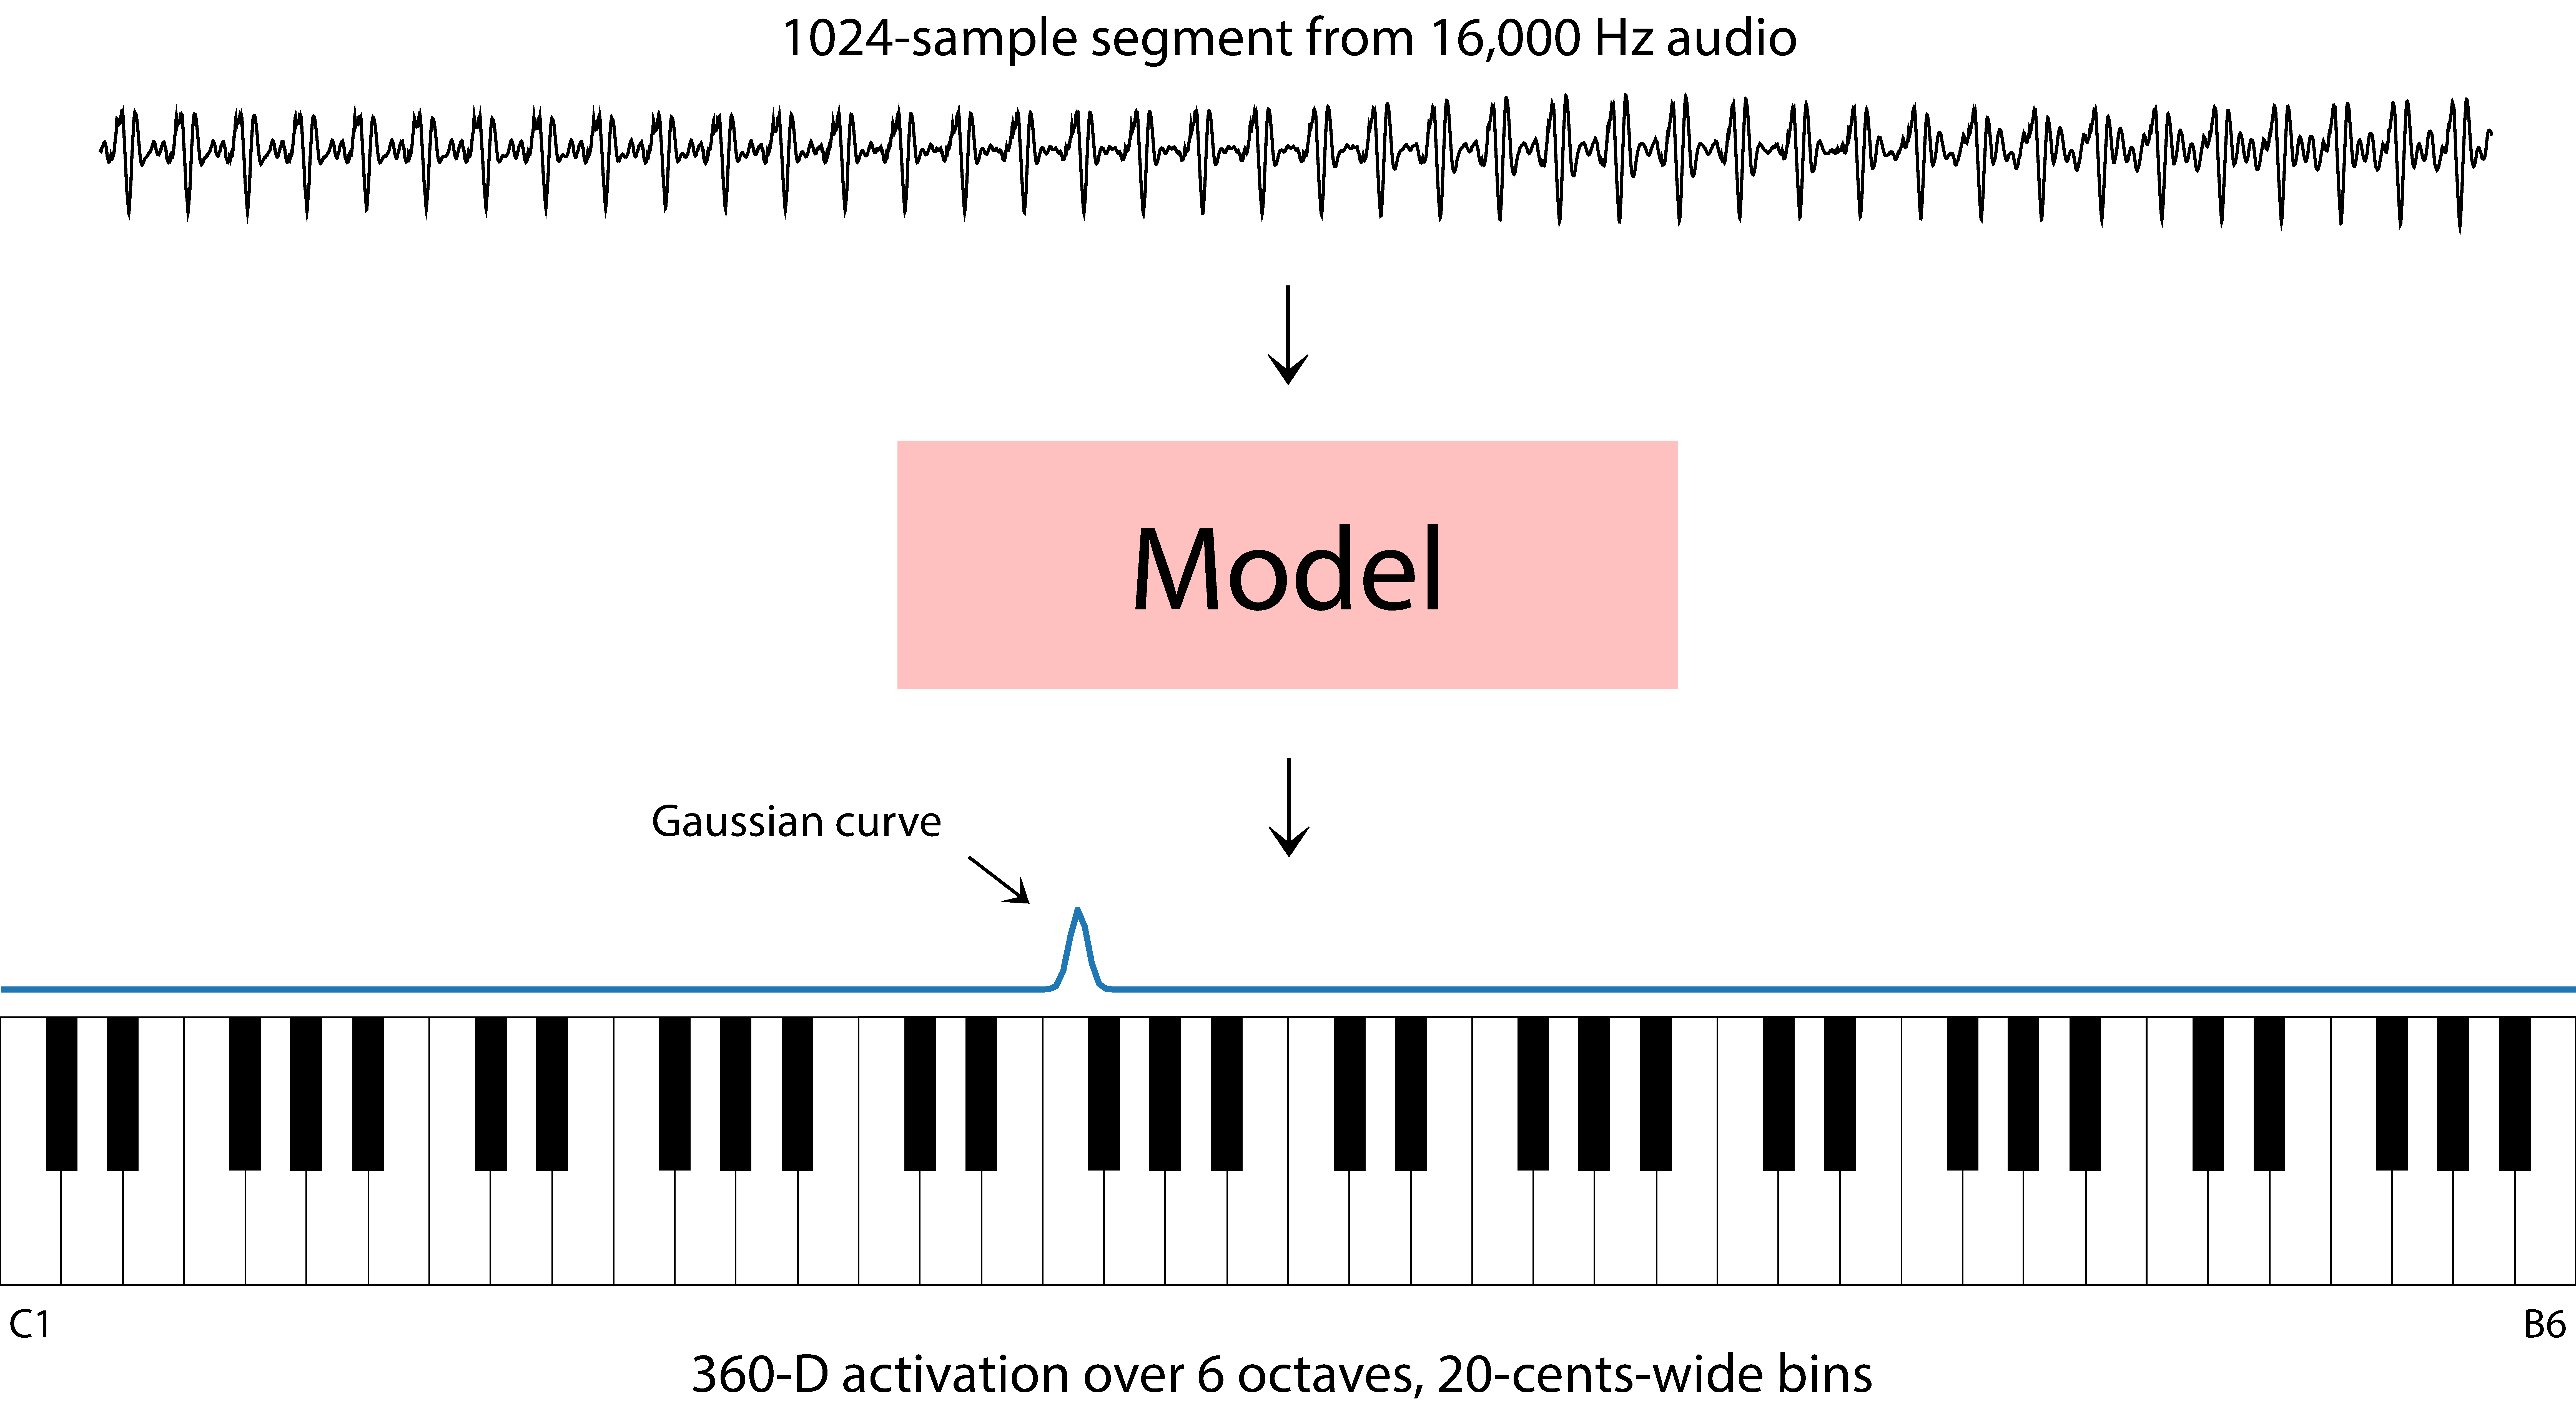
\includegraphics[width=0.9\linewidth]{formulation.pdf}
	\caption{The input and output representations of the CREPE model. The input is 1024 time-domain samples, and the output is a 360-dimensional vector that contains a Gaussian curve centered at the ground-truth frequency (see Equation \ref{eqn:gaussian}). For details on the convolutional architecture used in the model, see Figure \ref{fig:architecture}.}\label{fig:formulation}
\end{figure}

\begin{sidewaysfigure}
	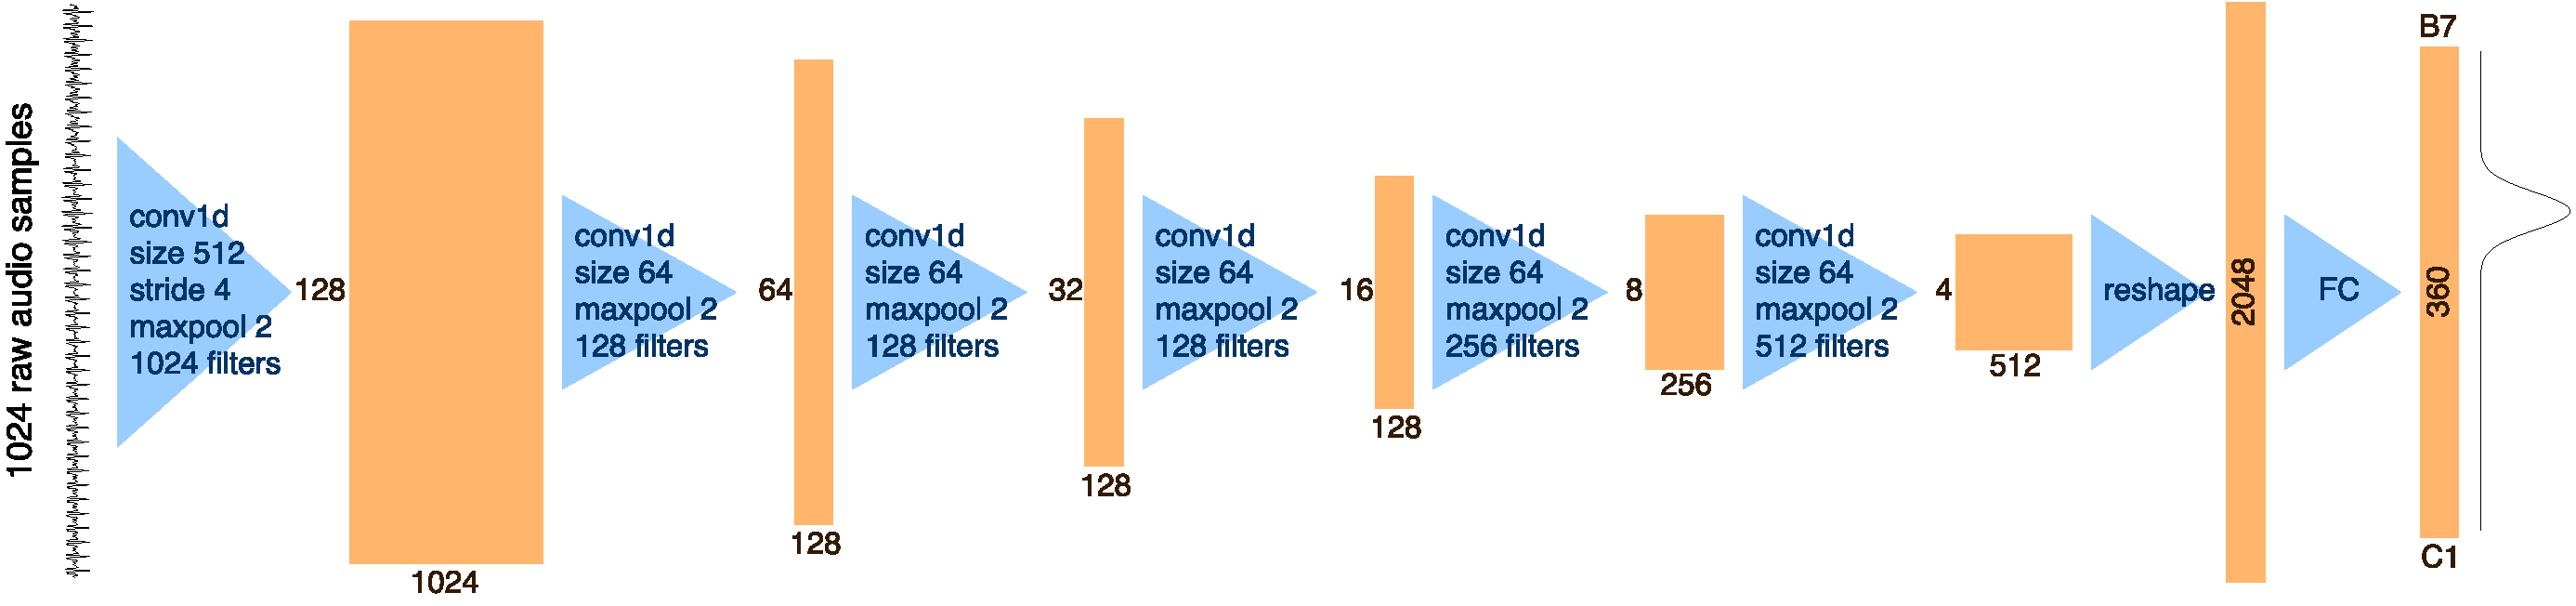
\includegraphics[width=\textwidth]{architecture.pdf}
	\caption{The architecture of the CREPE pitch tracker. The six convolutional layers predicts the Gaussian curve centered at the ground-truth frequency. The output is then used to extract the exact pitch estimate as in Equation \ref{eqn:resulting}-\ref{eqn:resulting2}.}
	\label{fig:architecture}
\end{sidewaysfigure}

CREPE consists of a deep convolutional neural network which operates directly on the time-domain audio signal to produce a pitch estimate.
The input and output representations used in the model are illustrated in Figure \ref{fig:formulation}.
The input is a 1024-sample excerpt from the time-domain audio signal, using a 16 kHz sampling rate, and the output is a 360-dimensional vector $\hat{\mathbf{y}}$, from which the resulting pitch estimate is calculated deterministically.

Each of the 360 dimensions in the output corresponds to a specific pitch value, defined in cents.
Cent is a unit representing musical intervals relative to a reference pitch $f_{\mathrm{ref}}$ in Hz, defined as a function of frequency $f$ in Hz:
\begin{equation}
\cent(f) = 1200 \cdot \log_2 \frac{f}{f_{\mathrm{ref}}},
\end{equation}
where $f_{\mathrm{ref}} = 10 \mathrm{~Hz}$ throughout the experiments. 
This unit provides a logarithmic pitch scale where 100 cents equal one semitone.
The 360 pitch values are denoted as $\cent_1, \cent_2, \cdots, \cent_{360}$ and are selected so that they cover six octaves with 20-cent intervals between C1 and B6, corresponding to 32.70 Hz and 1975.5 Hz. 
The resulting pitch estimate $\hat{\cent}$ is the weighted average of the associated pitches $\cent_i$ according to the output $\hat{\mathbf{y}}$, which gives the frequency estimate in Hz:
\begin{equation}\label{eqn:resulting}
\hat{\cent} = \frac{\sum_{i=1}^{360}\hat{y}_i \cent_i}{\sum_{i=1}^{360} \hat{y}_i},
\end{equation}
\begin{equation}\label{eqn:resulting2}
\hat{f} = f_{\mathrm{ref}} \cdot 2 ^ {\hat{\cent} / 1200}.
\end{equation}

The target outputs we use to train the model are 360-dimensional vectors, where each dimension represents a frequency bin covering 20 cents (the same as the model's output).
The bin corresponding to the ground truth fundamental frequency is given a magnitude of one.
As in \cite{bittner2017deepsalience}, in order to soften the penalty for near-correct predictions, the target is Gaussian-blurred in frequency such that the energy surrounding a ground truth frequency decays with a standard deviation of 25 cents:
\begin{equation}\label{eqn:gaussian}
y_i = \exp \left ( {-\frac{(\cent_i - \cent_{\mathrm{true}})^2}{2 \cdot 25^2}} \right ),
\end{equation}
This way, high activations in the last layer indicate that the input signal is likely to have a pitch that is close to the associated pitches of the nodes with high activations.

A detailed block diagram of the proposed architecture is provided in Figure \ref{fig:architecture}.
There are six convolutional layers that result in a 2048-dimensional latent representation, which is then connected densely to the output layer with sigmoid activations to produce the 360-dimensional target vector.
The network is trained to minimize the binary cross entropy between the target vector $\mathbf{y}$ and the predicted vector $\hat{\mathbf{y}}$:
\begin{equation}
\mathcal{L}(\mathbf{y}, \hat{\mathbf{y}}) = \sum_{i=1}^{360} \left ( - y_i \log \hat{y_i} - (1 - y_i) \log (1 - \hat{y_i}) \right ),
\end{equation}
where both $y_i$ and $\hat{y}_i$ are real numbers between 0 and 1.
This loss function is optimized using the ADAM optimizer \cite{kingma2015adam}, with the learning rate 0.0002. 
The best performing model is selected after training until the validation accuracy no longer improves for 32 epochs, where one epoch consists of 500 batches of 32 examples randomly selected from the training set. 
Each convolutional layer is preceded with batch normalization \cite{ioffe2015batchnorm} and followed by a dropout layer \cite{srivastava2014dropout} with the dropout probability 0.25.
This architecture and the training procedures are implemented using Keras \cite{chollet2015keras}.




\section{Experiments}

\subsection{Datasets}

In order to objectively evaluate CREPE and compare its performance to alternative algorithms, we require audio data with perfect ground truth annotations.
This is especially important since the performance of the compared algorithms is already very high.
In light of this, we cannot use a dataset such as MedleyDB \cite{bittner2014medleydb}, since its annotation process includes manual corrections which do not guarantee a 100\% perfect match between the annotation and the audio, and it can be affected, to a degree, by human subjectivity.
To guarantee a perfectly objective evaluation, we must use datasets of synthesized audio in which we have perfect control over the f0 of the resulting signal.
We use two such datasets: the first, RWC-synth, contains 6.16 hours of audio synthesized from the RWC Music Database \cite{goto2002rwc} and is used to evaluate pYIN in \cite{mauch2014pyin}.
It is important to note that the signals in this dataset were synthesized using a fixed sum of a small number of sinusoids, meaning that the dataset is highly homogenous in timbre and represents an over-simplified scenario.
To evaluate the algorithms under more realistic (but still controlled) conditions, the second dataset we use is a collection of 230 monophonic stems taken from MedleyDB and re-synthesized using the methodology presented in \cite{salamon2017analysis}, which uses an analysis/synthesis approach to generate a synthesized track with a perfect f0 annotation that maintains the timbre and dynamics of the original track.
This dataset consists of 230 tracks with 25 instruments, totaling 15.56 hours of audio, and henceforth referred to as MDB-stem-synth.


\subsection{Methodology}

We train the model using 5-fold cross-validation, using a 60/20/20 train, validation, and test split.
For MDB-stem-synth, we use artist-conditional folds, in order to avoid training and testing on the same artist which can result in artificially high performance due to artist or album effects \cite{sturm2013classification}.
The evaluation of an algorithm's pitch estimation is measured in raw pitch accuracy (RPA) and raw chroma accuracy (RCA) with 50 cent thresholds \cite{salamon2014melody}.
These metrics measure the proportion of frames in the output for which the output of the algorithm is within 50 cents (a quarter-tone) of the ground truth.
We use the reference implementation provided in \texttt{mir\_eval} \cite{raffel2014mir_eval} to compute the evaluation metrics.

We compare CREPE against the current state of the art in monophonic pitch tracking, represented by the pYIN \cite{mauch2014pyin} and SWIPE \cite{camacho2008swipe} algorithms.
To examine the noise robustness of each algorithm, we also evaluate their pitch tracking performance on degraded versions of MDB-stem-synth, using the Audio Degradation Toolbox (ADT) \cite{mauch2013adt}.
We use four different noise sources provided by the ADT: pub, white, pink, and brown.
The pub noise is an actual recording of the sound in a crowded pub, 
and the white noise is a random signal with a constant power spectral density over all frequencies.
The pink and brown noise have the highest power spectral density in low frequencies, and the densities fall off at 10 dB and 20 dB per decade respectively.
Seven different signal-to-noise ratio (SNR) values are used: $\infty$, 40, 30, 20, 10, 5, and 0 dB.


\subsection{Results}

\subsubsection{Pitch Accuracy}

Table \ref{tbl:accuracy50} shows the pitch estimation performance tested on the two datasets.
On the RWC-synth dataset, CREPE yields a close-to-perfect performance where the error rate is lower than the baselines by more than an order of magnitude.
While these high accuracy numbers are encouraging, those are achievable thanks to the highly homogeneous timbre of the dataset.
In order to test the generalizability of the algorithms on a more timbrally diverse dataset, the performance is evaluated on the MDB-stem-synth dataset as well.
It is notable that the degradation of performance from RWC-synth is more significant for the baseline algorithms, implying that CREPE is more robust to complex timbres compared to pYIN and SWIPE.

\begin{table}[t]
	\begin{center}
		\begin{tabular}{c|c||c|c|c} \hline
			\multicolumn{1}{c}{Dataset} & \multicolumn{1}{c}{Metric} & \multicolumn{1}{c}{CREPE} & \multicolumn{1}{c}{pYIN} & \multicolumn{1}{c}{SWIPE} \\ \hline
			\multirow{2}{*}{RWC-synth} & RPA & \textbf{0.999$\pm$0.002} & 0.990$\pm$0.006& 0.963$\pm$0.023 \\ \cline{2-5}
			& RCA & \textbf{0.999$\pm$0.002} & 0.990$\pm$0.006& 0.966$\pm$0.020 \\ \hline \hline
			\multirow{2}{*}{MDB-stem-synth} & RPA & \textbf{0.967$\pm$0.091} & 0.919$\pm$0.129& 0.925$\pm$0.116 \\ \cline{2-5}
			& RCA & \textbf{0.970$\pm$0.084} & 0.936$\pm$0.092& 0.936$\pm$0.100 \\ \hline
		\end{tabular}
	\end{center}
	\caption{Average raw pitch/chroma accuracies and their standard deviations, tested with the 50 cents threshold.}
	\label{tbl:accuracy50}
\end{table}

\begin{table}[t]
	\begin{center}
		\begin{tabular}{c|c||c|c|c} \hline
			\multicolumn{1}{c}{Dataset} & \multicolumn{1}{c}{Threshold} &  \multicolumn{1}{c}{CREPE} & \multicolumn{1}{c}{pYIN} & \multicolumn{1}{c}{SWIPE} \\ \hline
			
			\multirow{3}{*}{RWC-synth} 
			& 50 cents & \textbf{0.999$\pm$0.002} & 0.990$\pm$0.006 & 0.963$\pm$0.023 \\ \cline{2-5}
			& 25 cents & \textbf{0.999$\pm$0.003} & 0.972$\pm$0.012 & 0.949$\pm$0.026 \\ \cline{2-5}
			& 10 cents & \textbf{0.995$\pm$0.004} & 0.908$\pm$0.032 & 0.833$\pm$0.055 \\ \hline \hline
			
			\multirow{3}{*}{MDB-stem-synth}
			& 50 cents & \textbf{0.967$\pm$0.091} & 0.919$\pm$0.129 & 0.925$\pm$0.116 \\ \cline{2-5}
			& 25 cents & \textbf{0.953$\pm$0.103} & 0.890$\pm$0.134 & 0.897$\pm$0.127 \\ \cline{2-5}
			& 10 cents & \textbf{0.909$\pm$0.126} & 0.826$\pm$0.150 & 0.816$\pm$0.165 \\ \hline
		\end{tabular}
	\end{center}
	\caption{Average raw pitch accuracies and their standard deviations, with different evaluation thresholds.}
	\label{tbl:thresholds}
\end{table}

Finally, to see how the algorithms compare under scenarios where any deviation in the estimated pitch from the true value could be detrimental, Table \ref{tbl:thresholds} reports the RPA at lower evaluation tolerance thresholds of 10 and 25 cents as well as the RPA at the standard 50 cents threshold for reference.
The table indicates that as the threshold is decreased, the difference in performance becomes more accentuated, with CREPE outperforming by over 8 percentage points when the evaluation tolerance is lowered to 10 cents.
The high accuracy in 10 cents despite the 20-cent resolution of the model output indicates that the weighted average solution in Equation \ref{eqn:resulting} is effective at predicting the precise frequencies even between the adjacent frequency bins.
This suggests that CREPE is especially preferable when even minor deviations from the true pitch should be avoided as best as possible.
Obtaining highly precise pitch annotations is perceptually meaningful for transcription and analysis/resynthesis applications.


\subsubsection{Noise Robustness}


Noise robustness is key to many applications like speech analysis for mobile phones or smart speakers, or for live music performance.
Figure \ref{fig:noise} shows how the pitch estimation performance is affected when an additive noise is present in the input signal.
CREPE maintains the highest accuracy for all SNR levels for pub noise and white noise, and for all SNR levels except for the highest level of pink noise.
Brown noise is the exception where pYIN's performance is almost unaffected by the noise.
This can be attributed to the fact that brown noise has most of its energy at low frequencies, to which the YIN algorithm (on which pYIN is based) is particularly robust.

\begin{sidewaysfigure}
	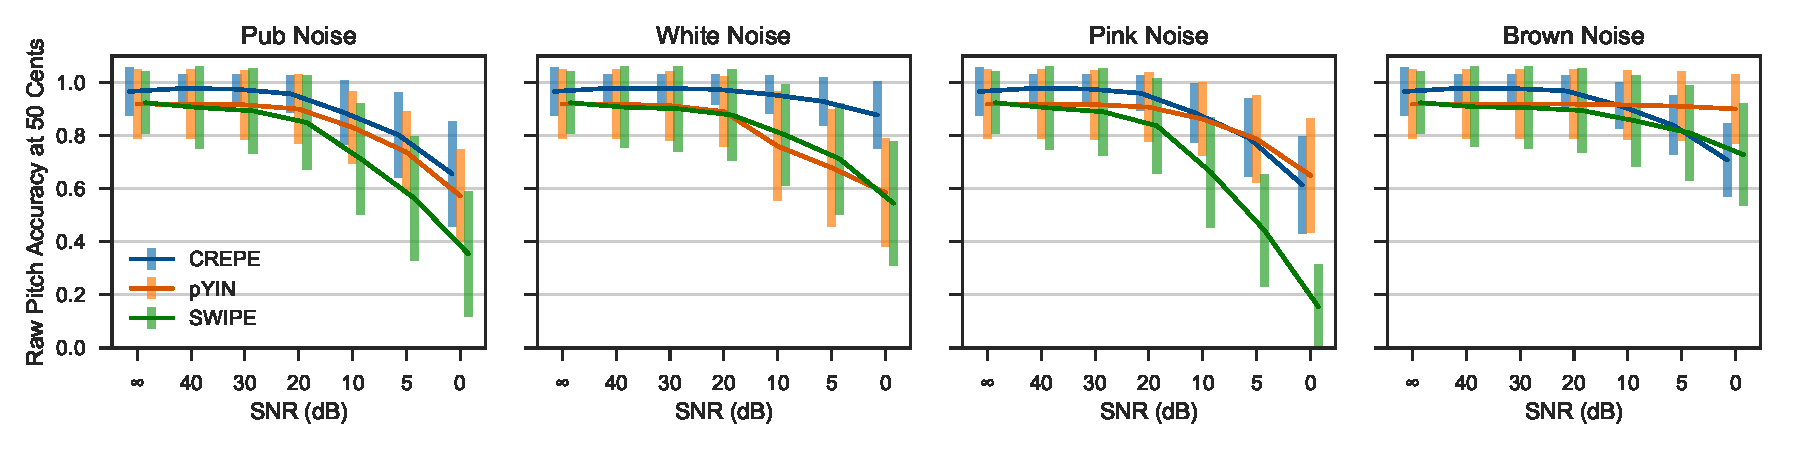
\includegraphics[width=\textwidth]{noise.pdf}
	\caption{Pitch tracking performance when additive noise signals are present. The error bars are centered at the average raw pitch accuracies and span the first standard deviations. With brown noise being a notable exception, CREPE shows the highest noise robustness in general. }
	\label{fig:noise}
\end{sidewaysfigure}

To summarize, CREPE performs better in all cases where the SNR is below 10 dB while the performance varies depending on the spectral properties of the noise when the noise level is higher, which indicates that this approach can be reliable under a reasonable amount of additive noise.
CREPE is also more stable, exhibiting consistently lower variance in performance compared to the baseline algorithms.


\begin{figure}
	\begin{minipage}{\columnwidth}
		\begin{center}
			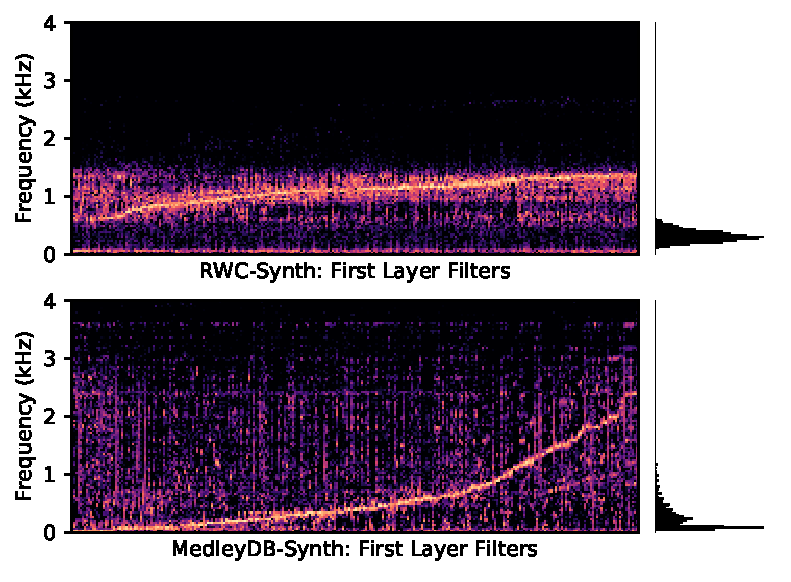
\includegraphics[width=0.8\columnwidth]{firstlayer-45.pdf}
		\end{center}
		\vspace{-10pt}
		\caption{
			Fourier spectra of the first-layer filters sorted by the frequency of the peak magnitude.
			Histograms on the right show the distribution of ground-truth frequencies in the corresponding dataset.
		}
		\label{fig:firstlayer}
	\end{minipage}
	\\ \vspace{2em} \\ 
	\begin{minipage}{\columnwidth}
		\begin{center}
			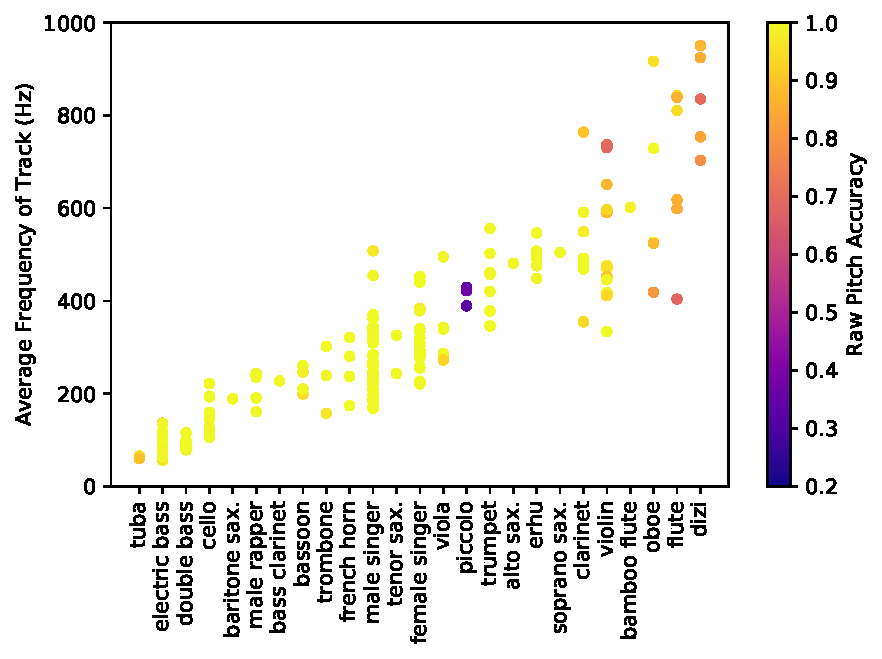
\includegraphics[width=0.8\columnwidth]{per-track-inst-45.pdf}
		\end{center}
		\vspace{-10pt}
		\caption{
			The raw pitch accuracy (RPA) of CREPE's predictions on each of the 230 tracks in MDB-stem-synth with respect to the instrument, sorted by the average frequency.
			% The  low-performing  cases  are  concentrated  in  the extreme frequencies, showing that the model performs better for the sfrequency range that are well-represented in the training set.
		}
		\label{fig:per-track}
	\end{minipage}
\end{figure}


\subsubsection{Model Analysis}

To gain some insight into the CREPE model, we visualize in Figure \ref{fig:firstlayer} the spectra of the 1024 convolutional filters in the first layer of the neural network, with histograms of the ground-truth frequencies to the right of each plot.
It is noticeable that the filters learned from the RWC-synth dataset have the spectral density concentrated between 600 Hz and 1500 Hz, while the ground-truth frequencies are mostly between 100 Hz and 600 Hz.
This indicates that the first convolutional layer in the model learns to distinguish the frequencies of the overtones rather than the fundamental frequency.
These filters focusing on overtones are also visible for MDB-stem-synth, where peak frequencies of the filters range well above the f0 distribution of the dataset, but in this case, the majority of the filters overlap with the ground-truth distribution, unlike RWC-synth.
A possible explanation for this is that since the timbre in RWC-synth is fixed and identical for all tracks, the model is able to obtain a highly accurate estimate of the f0 by modeling its harmonics.
Conversely, when the timbre is heterogeneous and more complex, as is the case for MDB-stem-synth, the model cannot rely solely on the harmonic structure and requires filters that capture the f0 periodicity directly in addition to the harmonics.
In both cases, this suggests that the neural network can adapt to the distribution of timbre and frequency in the dataset of interest, which in turn contributes to the higher performance of CREPE compared to the baseline algorithms.

\subsubsection{Performance by Instrument}

The MDB-stem-synth dataset contains 230 tracks from 25 different instruments, where electric bass (58 tracks) and male singer (41 tracks) are the most common while there are instruments that occur in only one or two tracks.
Figure \ref{fig:per-track} shows the performance of CREPE on each of the 230 tracks, with respect to the instrument of each track.
It is notable that the model performs worse for the instruments with higher average frequencies, but the performance is also dependent on the timbre.
CREPE performs particularly worse on the tracks with the dizi, a Chinese transverse flute, because the tracks came from the same artist, and they are all placed in the same split.
This means that for the fold in which the dizi tracks are in the test set, the training and validation sets do not contain a single dizi track, and the model fails to generalize to this previously unseen timbre.
There are 5 instruments (bass clarinet, bamboo flute, and the family of saxophones) that occur only once in the dataset, but their performance is decent, because their timbres do not deviate too far from other instruments in the dataset.
For the flute and the violin, although there are many tracks with the same instrument in the training set, the performance is low when the sound in the tested tracks is too low (flute) or too high (violin) compared to other tracks of the same instruments.
The low performance on the piccolo tracks is due to an error in the dataset where the annotation is inconsistent with the correct pitch range of the instrument.
Unsurprisingly, the model performs well on test tracks whose timbre and frequency range are well-represented in the training set.

\section{Open-Sourcing CREPE}

Releasing an implementation of research work as an open-source software helps ensure better quality, reproducibility, and longevity of the research code~\cite{mcfee2019opensource}.
To facilitate easier adoption of CREPE's pitch tracking functionality for wider audience, we open-sourced\footnote{\url{https://github.com/marl/crepe}} the implementation of CREPE under the MIT License.
The main purpose of the open-source release is to make the usage of the CREPE software as easy and effective as possible, so we aimed to ensure that the pitch estimation can work accurately for the broad range of the real-world monophonic signals.
As shown in Figure \ref{fig:firstlayer}, a model trained on a specific dataset specializes to the characteristics of the sounds in the dataset and will fail to work well across the previously unknown, real-world inputs.
To address this problem, we used six different datasets for the pre-trained model included in the open-source release of CREPE: MIR-1K~\cite{hsu2010mir1k}, Bach10~\cite{duan2010bach10}, RWC-Synth~\cite{mauch2014pyin}, MedleyDB~\cite{bittner2014medleydb}, MDB-STEM-Synth~\cite{salamon2017analysis}, and NSynth~\cite{engel2017nsynth}.
These datasets contain various instrumental and vocal sounds, and the pre-trained model is expected to work well on these types of sounds.
A visualization of the first-layer filters for the model trained with these datasets are shown in Figure \ref{fig:firstlayer-one}.
Compared to Figure \ref{fig:firstlayer}, the peak-frequency curve better covers the full range of frequencies and in a smoother manner.
An interesting feature of this visualization is that the curve is somewhat linear until 1 kHz and rapidly grows for the higher frequencies.
This roughly coincides with the Mel scale, where the mapping from the perceived frequency to the actual frequency is linear below 1 kHz and logarithmic above~\cite{logan2000mfcc}.


\begin{figure}
	\centering
	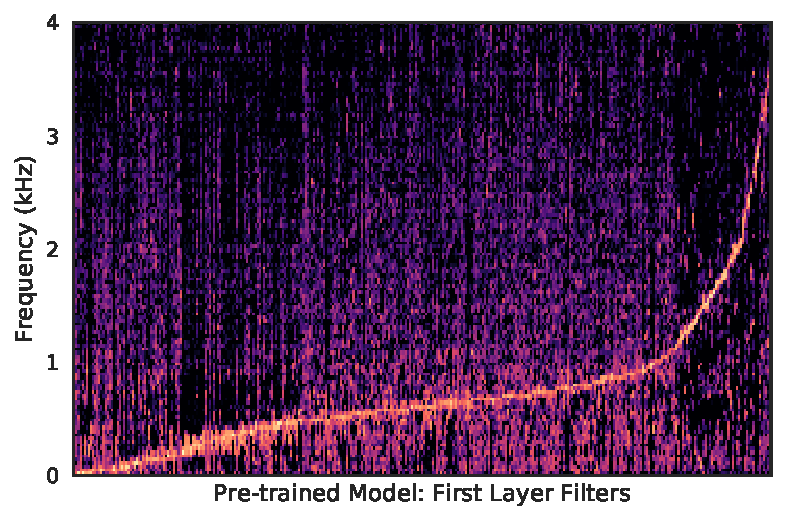
\includegraphics[width=0.6\textwidth]{firstlayer-one.pdf}
	\caption{The first layer filters of the CREPE model trained with six different datasets, visualized using the same method as in Figure \ref{fig:firstlayer}. Compared to the previous cases where the filters are specialized to one dataset, the peak-frequency curve is smoother and covers the full frequency range.}\label{fig:firstlayer-one}
\end{figure}

\subsection{Python Package and Command-Line Interface}

CREPE is distributed as a Python package and is hosted on the Python Package Index (PyPI). It can be installed simply by running the following command:

\vspace{1em}
\texttt{\$ pip install crepe}
\vspace{1em}

\noindent in a Python environment. This command will install the Python package \texttt{crepe} usable in Python scripts as well as a command-line interface that can be called with one or more audio file names:

\vspace{1em}
\texttt{\$ crepe audio\_file.wav}
\vspace{1em}

\noindent The estimated pitch values are saved using the CSV format, like:

\begin{figure}[b]
	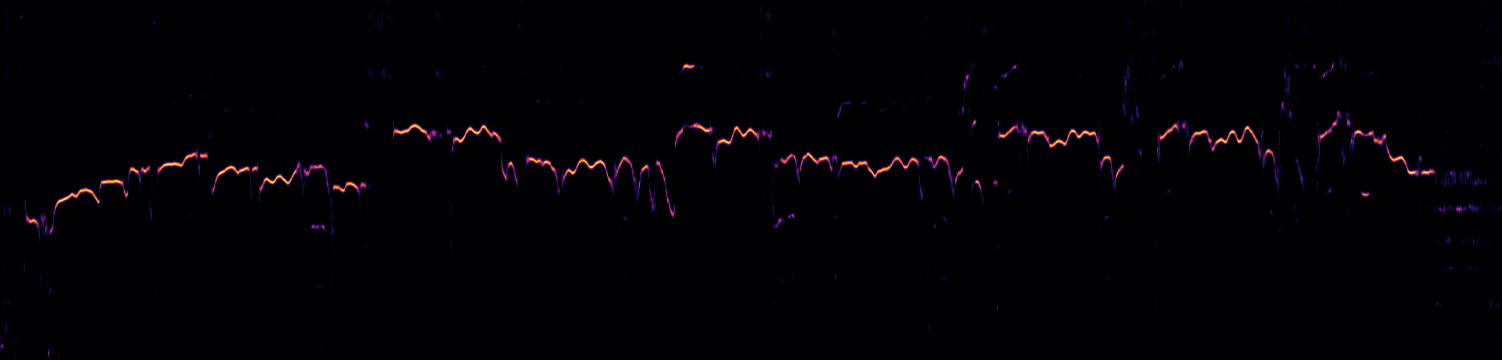
\includegraphics[width=\linewidth]{activation.png}
	\caption{Visualization of the target activation, which can be saved as in image file by using the \texttt{--save-activation} option in the CREPE command-line interface. The audio clip used contains an excerpt of male singing voice.}\label{fig:crepe-activation}
\end{figure}

\vspace{1em}
\texttt{time,frequency,confidence}

\texttt{0.00,185.616,0.907112}

\texttt{0.01,186.764,0.844488}

\texttt{0.02,188.356,0.798015}

\texttt{0.03,190.610,0.746729}

\texttt{0.04,192.952,0.771268}

\texttt{0.05,195.191,0.859440}

\texttt{0.06,196.541,0.864447}

\texttt{0.07,197.809,0.827441}

\texttt{0.08,199.678,0.775208}

\texttt{...}
\vspace{1em}

\noindent where the third column indicates the confidence level of the presence of a pitch, which is obtained by taking the maximum activation value at each frame.

The command-line interface supports various options, such as to use Viterbi smoothing~\cite{viterbi1967decoding} of the pitch curves as in pYIN~\cite{mauch2014pyin} and to save the activation in an image file as shown in Figure \ref{fig:crepe-activation}.
The package contains five pre-trained models with different capacities, where the number of convolutional channels are scaled to 12.5\% (tiny), 25\% (small), 50\% (medium), 75\% (large), or 100\% (full) relative to the model size used in the experiments (see Figure \ref{fig:architecture}), and the specific model capacity to use can be specified using the \texttt{--model-capacity} option.
Smaller-capacity models run significantly faster than the full-capacity model, suitable for resource-constrained use cases where faster computation is preferred at the cost of slightly lower pitch estimation accuracy.


\subsection{Real-Time Web Demo}

In addition to the Python package, we have developed a real-time web demo\footnote{\url{https://marl.github.io/crepe}} where the CREPE model runs on the web browser using the audio recorded from the system microphone and displays the target activation as well as the predicted pitch value in real time.
To enable this, the demo used the W3C Web Audio API for real-time audio input and TensorFlow.js~\cite{smilkov2019tensorflowjs} for running inference on the deep model.
Under the hood, TensorFlow.js uses WebGL which allows GPU acceleration for faster computation of the convolutional layers.
The web demo uses the ``tiny" capacity model in order to run faster in browsers, which uses less than 3\% of the parameters compared to the full model.
The web demo is also open-source and distributed in the same Github repository as the Python package.

\subsection{Argmax-Local Weighted Averaging}

In the process of training the model with diverse datasets, we have observed a side-effect where the model produces more octave errors, i.e. the predicted pitch is an octave apart from the ground truth.
These errors resulted in multiple peaks in the target output vector around the harmonics of the ground-truth frequency, as depicted in Figure \ref{fig:octave-errors}.
When the weighted average over the all 360 bins is used, this ends up predicting a completely different pitch.
To alleviate this, we have revised Equation \ref{eqn:resulting} in the open-source version of CREPE to calculate the weighted average using only the frequency bins around the highest peak in the output:
\begin{equation}\label{eqn:resulting-fixed}
\hat{\cent} = \frac{\sum\limits_{i=m-4}^{m+4}\hat{y}_i \cent_i}{\sum\limits_{i=m-4}^{m+4} \hat{y}_i},
~~~~~~~~~ m = \argmax_i \hat{y}_i.
\end{equation}
Using Equation \ref{eqn:resulting-fixed} improved the transcription accuracies of real-world signals significantly. However, a quantitative evaluation of the robustness in the real-world situations is inherently difficult and is out of the scope of this chapter, because it is virtually impossible to obtain a representative and objective dataset encompassing all such situations.

\begin{figure}
	\centering
	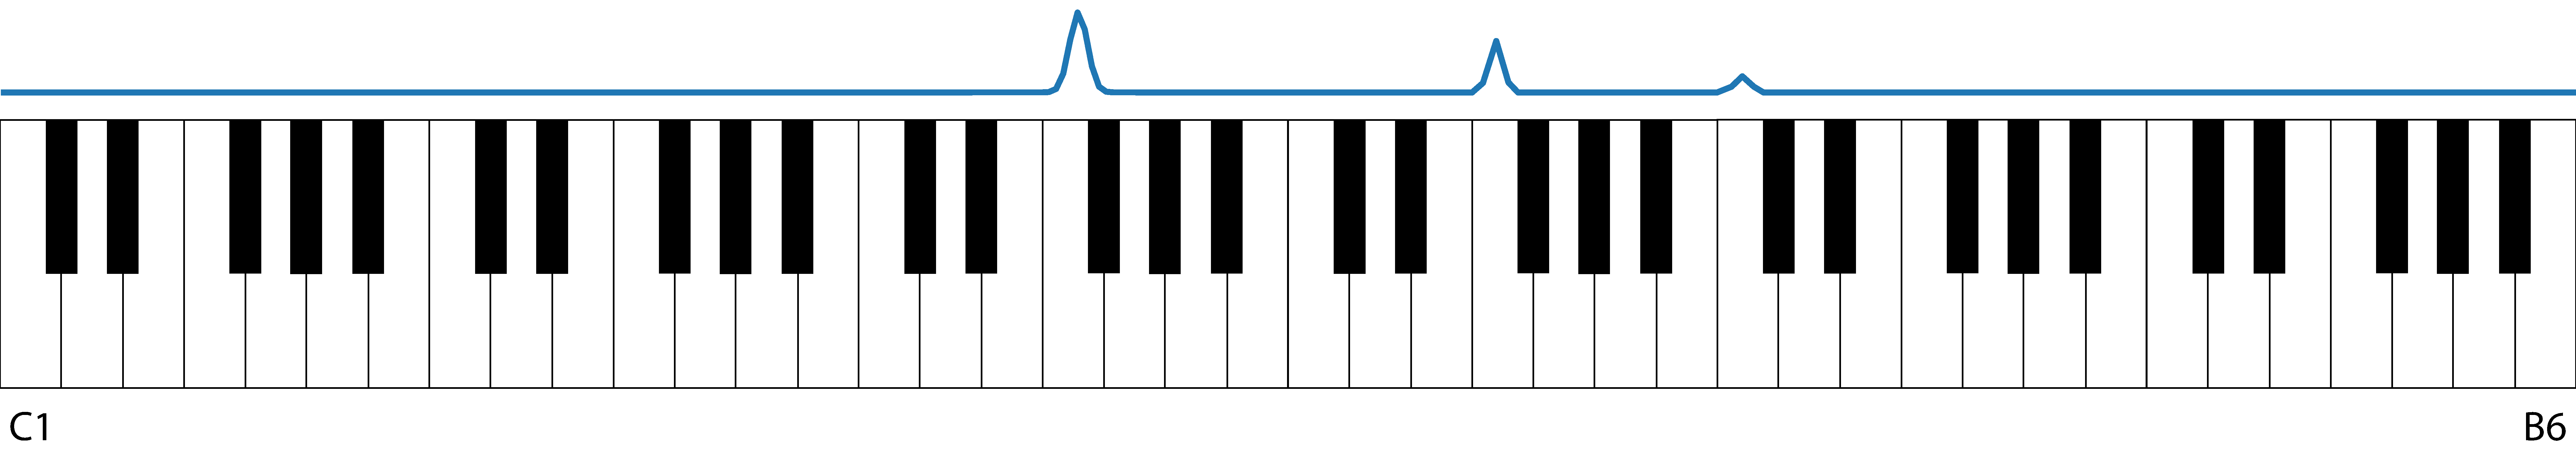
\includegraphics[width=\textwidth]{octave-errors.pdf}
	\caption{An example of an inaccurate target output where there exist multiple peaks around the harmonics of the ground-truth frequency. Equation \ref{eqn:resulting-fixed} ensures that the predicted pitch is calculated using only the frequency bins around the highest peak.}\label{fig:octave-errors}
\end{figure}

\subsection{Data-Driven Models and Real-World Applications}

The series of modifications on the CREPE model are taken in order to release the open-source software that are effective not only for evaluation in an academic setting but also in various real-world scenarios of pitch estimation.
These give an important lesson that should be considered when developing data-driven models for music analysis tasks.
Especially with the rise of deep learning models that typically have a large number of parameters, it is very easy to overfit a model to work well with a specific dataset while not being able to generalize.
This problem can persist even if the dataset is properly splitted for training and evaluation, because it is common for such dataset to have shared characteristics such as recording and mixing conditions that are not particularly representative of the broad range of the real-world data for which the model should supposedly work well.
Therefore, a great amount of care should be taken when selecting the datasets to be used for evaluation of a music analysis model, and qualitative analyses on out-of-distribution real-world data need to be accompanied.


\section{Conclusions}

In this chapter, we presented a novel data-driven method for monophonic pitch tracking based on a deep convolutional neural network operating on time-domain input, CREPE.
We showed that CREPE obtains state-of-the-art results, outperforming pYIN and SWIPE on two datasets with homogeneous and heterogeneous timbre respectively.
Furthermore, we showed that CREPE remains highly accurate even at a very strict evaluation threshold of just 10 cents.
We also showed that in most cases CREPE is more robust to added noise.
In addition, we discussed the challenges that arose during the open-source release of the model, which included how to make the model more generalizable to the real-world sounds and the revised pitch extraction strategy to better deal with increased octave errors.

Ideally, we want the model to be invariant to all transformations that do not affect pitch, such as changes due to distortion and reverberation.
Some invariance can be induced by the architectural design of the model, such as the translation invariance induced by pooling layers in our model as well as in deep image classification models.
However, it is not as straightforward to design the model architecture to specifically ignore other pitch-preserving transformations.
While it is still an intriguing problem to build an architecture to achieve this, we could use data augmentation to generate transformed and degraded inputs that can effectively make the model learn the invariance.
The robustness of the model could also be improved by applying pitch-shifts as data augmentation \cite{mcfee2015muda} to cover a wider pitch range for every instrument.
In addition to data augmentation, various sources of audio timbre can be obtained from software instruments; NSynth \cite{engel2017nsynth} is an example where the training dataset is generated from the sound of software instruments.


Pitch values tend to be continuous over time, but CREPE estimates the pitch of every frame independently without using any temporal tracking, unlike pYIN which exploits this by using an HMM to enforce temporal smoothness.
We can potentially improve the performance of CREPE further by statistically modeling how the pitch value changes over time.
Employing recurrent neural networks (RNNs) is a natural choice for this, and we will explore in the following chapters how RNNs can model the temporal characteristics of music, focusing on two specific tasks: music synthesis (Chapter \ref{ch:synthesis}) and piano transcription (Chapter \ref{ch:adversarial}).



%!TEX root = ../dissertation.tex
% this file is called up by thesis.tex
% content in this file will be fed into the main document

\graphicspath{{5-synthesis/figures/}}

\chapter{Learning Timbre Space for Music Synthesis}
\label{ch:synthesis}

The recent success of raw audio waveform synthesis models like WaveNet motivates a new approach for music synthesis, in which the entire process --- creating audio samples from a score and instrument information --- is modeled using generative neural networks.
This paper describes a neural music synthesis model with flexible timbre controls, which consists of a recurrent neural network conditioned on a learned instrument embedding followed by a WaveNet vocoder.
The learned embedding space successfully captures the diverse variations in timbres within a large dataset and enables timbre control and morphing by interpolating between instruments in the embedding space.
The synthesis quality is evaluated both numerically and perceptually, and an interactive web demo is presented.


\section{Introduction}

Musical synthesis, most commonly, is the process of generating musical audio with given control parameters such as instrument type and note sequences over time.
The primary difference between synthesis engines is the way in which \emph{timbre} is modeled and controlled.
In general, it is difficult to design a synthesizer that both has dynamic and intuitive timbre control and is able to span a wide range of timbres; most synthesizers change timbres by having presets for different instrument classes or have a very limited space of timbre transformations available for a single instrument type.

In this paper, we present a flexible music synthesizer named Mel2Mel, which uses a learned, non-linear instrument embedding as timbre control parameters in conjunction with a learned synthesis engine based on WaveNet.
Because the model has to learn the timbre -- any information not specified in the note sequence -- to successfully reconstruct the audio, the embedding space spans over the various aspects of timbre such as spectral and temporal envelopes of notes.
This learned synthesis engine allows for flexible timbre control, and in particular, timbre morphing between instruments, as demonstrated in our interactive web demo.\footnote{\url{https://neural-music-synthesis.github.io}}

% \section{Background}\label{sec:background}

\subsection{Timbre Control in Musical Synthesis}

Methods for music synthesis are based on a variety of techniques such as FM synthesis, subtractive synthesis, physical modeling, sample-based synthesis, and granular synthesis~\cite{pejrolo2017creating}.
The method of controlling timbre and the level of flexibility depends on the parameters of the exact method used, but in general, there is a trade-off between flexible timbre control over synthetic sounds (e.g. FM or subtractive synthesis) and a limited timbre control in more ``realistic'' sounds (e.g. sample-based or granular synthesis). %\textsuperscript{\note{citation needed}}
Our work is aimed at achieving the best of both worlds: flexibly controlling a variety of realistic-sounding timbres.

\pagebreak

\subsection{Timbre Morphing}

`Morphing' of a sound can be generally described as making a perceptually gradual transition between two or more sounds~\cite{caetano2010automatic}.
A common approach is to use a synthesis model and define sound morphing as a numerical interpolation of the model parameters.
Sinusoidal models can directly interpolate between the energy proportions of the partials~\cite{osaka1995timbre,boccardi2001sound}.
Other models use parameters characterizing the spectral envelope~\cite{slaney1996automatic,ezzat2005morphing} or psychoacoustic features for perceptually linear transition~\cite{caetano2013musical}.
A limitation of these approaches is that morphing can only be applied among the range of timbres covered by a certain synthesis model, whose expressiveness or parameter set may be limited.
To overcome this, we employ a data-driven approach for music synthesis that is generalizable to all timbres in the dataset.

\subsection{Timbre Spaces and Embeddings}

Timbre is often modeled using a timbre space~\cite{peeters2011timbre}, in which similar timbres lie closer than dissimilar timbres.
In psychoacoustics, multidimensional scaling (MDS) is used to obtain a timbre space which preserves the timbral dissimilarities measured in perceptual experiments~\cite{grey1977multidimensional,wessel1979timbre}.
Meanwhile, in music content analysis, timbre similarity is measured using computed features such as the Mel-frequency cepstral coefficients (MFCCs) \cite{logan2000mfcc},
descriptors of the spectral envelope \cite{agostini2013aid}, or hidden-layer weights of a neural network trained to distinguish different timbres~\cite{humphrey2011nlse}.
A recent method~\cite{esling2018timbre} used a variational autoencoder \cite{kingma2014vae} to obtain a timbre space, and unlike the above embeddings, the method is able to generate monophonic audio for a particular timbre embedding but does not consider the temporal evolution of notes such as attacks and decays.
In our work, we generate a timbre embedding as a byproduct of polyphonic synthesis, which can utilize both spectral and temporal aspects of timbres.


\subsection{Neural Audio Synthesis using WaveNet}

WaveNet~\cite{oord2016wavenet} is a generative audio synthesis model that is able to produce realistic human speech.
WaveNet achieves this by learning an autoregressive distribution which predicts the next audio sample from the previous samples in its receptive field using a series of dilated convolutions.
Tacotron~\cite{shen2018tacotron} and Deep Voice~\cite{ping2018deepvoice3} are WaveNet-based text-to-speech models which first predict a Mel spectrogram from text and use it to condition a WaveNet vocoder.

There are also a few notable applications of WaveNet on music, including NSynth~\cite{engel2017nsynth}, an autoencoder architecture which separately encodes monophonic pitch with learned timbral features, and the universal music translation network~\cite{mor2019universal} which uses a denoising autoencoder architecture that can extract and translate between musical styles while preserving the melody.
In \cite{hawthorne2019maestro}, a WaveNet is used for music synthesis conditioned directly on note sequences, while only supporting piano sounds.
Our model is similarly built around WaveNet for its synthesis capability, while using a learned embedding space to flexibly control the timbre of polyphonic music.


\pagebreak % temp 

\section{Method}\label{sec:method}

The neural network shown in Figure \ref{fig:mel2mel-architecture}, dubbed Mel2Mel, concerns the task of synthesizing music corresponding to given note sequences and timbre.
The note sequences are supplied as a MIDI file and converted to a piano roll representation, which contains the note timings and the corresponding note velocities for each of the 88 piano keys.
We use a fixed step size in time, and the piano roll representation is encoded as a matrix by quantizing the note timings to the nearest time step.
The input to the neural network is a concatenation of two 88-dimensional piano roll representations, one for onsets and one for frames, comprising 176 dimensions in total:
\begin{eqnarray*}
	\mathbf{X} & =&  [~ \mathbf{X}^{\textrm{onset}} ~;~ \mathbf{X}^{\textrm{frame}} ~] \\
	\mathbf{X}^{\textrm{onset}}_{p,t} &= & v_{\textrm{~the active note}} \cdot \mathbb{1}_{\textrm{a note at pitch $p$ is \textit{first} active at time $t$}} \\
	\mathbf{X}^{\textrm{frame}}_{p,t} &= & v_{\textrm{~the active note}} \cdot \mathbb{1}_{\textrm{a note at pitch $p$ is active at time $t$}}
\end{eqnarray*}
\noindent where $\mathbb{1}$ is the indicator function, and $v$ denotes the MIDI velocity scaled to $[0, 1]$.
This input representation is inspired by \cite{hawthorne2018onsetsframes} which showed that jointly training on onsets and frames performs better than using frame information only;
similarly, we want the network to maximally utilize the onsets which have the most relevant information on the attack sounds, while still receiving the frame information.
Another reason for using both onsets and frames is that, because of the time quantization, repeated notes become indistinguishable only using $\mathbf{X}^\textrm{frame}$ when an offset is too close to the subsequent onset.

The input goes through a linear 1x1 convolution layer, which is essentially a time-distributed fully connected layer, followed by a FiLM layer, to be described in the following subsection, which takes the timbre embedding vector and transforms the features accordingly.
After a bidirectional LSTM layer and another FiLM layer for timbre conditioning, another linear 1x1 convolution layer produces the Mel spectrogram prediction.
The resulting Mel spectrogram is then fed to a WaveNet vocoder to produce the music; Mel spectrograms compactly convey sufficient information for audio synthesis and have been successfully used for conditioning WaveNet~\cite{shen2018tacotron,ping2018deepvoice3}.
The use of bidirectional LSTM is justified because Mel spectrograms are constructed using a larger window than the step size, making it non-causal.
The only nonlinearities in the network are in the LSTM, and there are no time-domain convolutions except in WaveNet.


\subsection{Timbre Conditioning using FiLM Layers}

We can think of this architecture as a multi-step process that shapes a piano roll into its Mel spectrogram, by applying appropriate timbre given as side information.
A FiLM layer~\cite{perez2018film} is a suitable choice for this task, because it can represent such action of shaping using an affine transformation of intermediate-layer features.
For each instrument to model, its timbre is represented in an embedding vector $\mathbf{t}$, implemented as a learned matrix multiplication on one-hot encoded instrument labels.
A FiLM layer learns functions $f$ and $h$, which are simply linear layers mapping the timbre embedding $\mathbf{t}$ to $\gamma = f ( \mathbf{t} )$ and $\beta = h ( \mathbf{t} )$.
The affine transformation, or FiLM-ing, of intermediate-layer features $\mathbf{F}$ is then applied using feature-wise operations: $
\mathrm{FiLM}(\mathbf{F} ~|~ \gamma, \beta)
= \gamma \mathbf{F} + \beta
= f(\mathbf{t})\mathbf{F} + h(\mathbf{t}). $

At a higher level, the affine transformations learned by the FiLM layers are nonlinearly transformed by the recurrent and convolutional layers to respectively form temporal and spectral envelopes, which are two important aspects that characterize instrumental timbre.
Using the first FiLM layer is essential because the recurrent layer needs to take timbre-dependent input to apply the temporal dynamics according to the timbre, and the second FiLM layer can apply additional spectral envelope on the recurrent layer's output.

\begin{figure}[t]
	\centering
	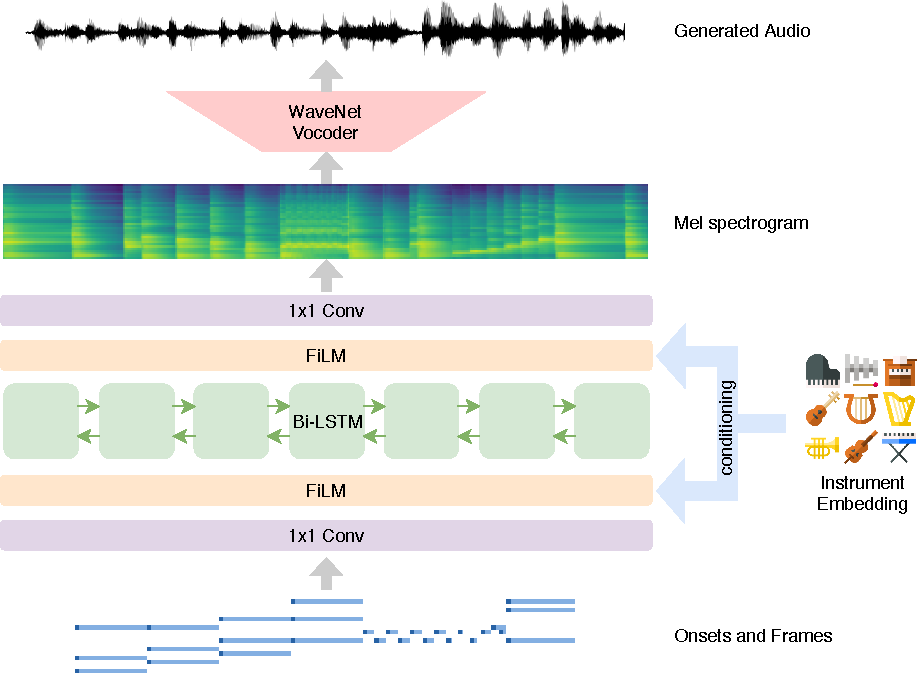
\includegraphics[width=\linewidth]{architecture.pdf}
	\caption{The overall architecture of the proposed Mel2Mel model. The note sequences and instrument embeddings are combined to predict the Mel spectrogram, which is then fed to the WaveNet vocoder.}
	\label{fig:mel2mel-architecture}
\end{figure}

\subsection{Model Details}

The sampling rate of 16 kHz and $\mu$-law encoding with 256 quantization levels are used for all audio as in the original WaveNet paper~\cite{oord2016wavenet}.
The predicted Mel spectrograms are defined using 80 area-normalized triangular filters distributed evenly between zero and the Nyquist frequency in the Mel scale.
The STFT window length of 1,024 samples and the step size of 128 samples are used, which translate to 64 milliseconds and 8 milliseconds, respectively.
Unless specified otherwise, we use 256 channels in all hidden layers and a two-dimensional embedding space for timbre conditioning.

For Mel spectrogram prediction, an Adam optimizer with the initial learning rate of 0.002 is used, and the learning rate is halved every 40,000 iterations.
The model is trained for 100,000 iterations, where each iteration takes a mini-batch of 128 sequences of length 65,536, or 4.096 seconds.
Three different loss functions are used and compared; for linear-scale Mel spectrograms $S_{\mathrm{true}}$ and $S_{\mathrm{pred}}$:
\begin{align}
\footnotesize \textbf{abs MSE} & ~=~ \mathbb{E} \left [ \left ( S_{\mathrm{true}} - S_{\mathrm{pred}} \right )^2 \right ]
\label{eqn:abs-loss} \\
\footnotesize \textbf{log-abs MSE} & ~=~ \mathbb{E} \left [ \left ( \log S_{\mathrm{true}} - \log S_{\mathrm{pred}} \right )^2 \right ]
\label{eqn:log-abs-loss} \\
\footnotesize \textbf{tanh-log-abs MSE} & ~=~ \mathbb{E} \left [ \left ( \tanh \tfrac{1}{4}\log S_{\mathrm{true}} - \tanh \tfrac{1}{4}\log S_{\mathrm{pred}}  \right )^2 \right ]
\label{eqn:tanh-log-abs-loss}
\end{align}
\noindent All logarithms above are natural, and the spectrogram magnitudes are clipped at -100 dB. Prepending $\tanh$ gives a soft-thresholding effect where the errors in the low-energy ranges are penalized less than the errors close to 0 dB.

For the WaveNet vocoder, we used nv-wavenet\footnote{\url{https://github.com/NVIDIA/nv-wavenet}}, a real-time open-source implementation of autoregressive WaveNet by NVIDIA.
This implementation limits the recurrent channel size at 64 and the skip channels at 256, because of the GPU memory capacity.
% Although nv-wavenet is autoregressive and slower than Parallel WaveNet, it allows faster-than-real-time synthesis without separately training a student WaveNet through inverse autoregressive flows.
A 20-layer WaveNet model was trained with the maximum dilation of 512, and the Mel spectrogram input is upsampled using two transposed convolution layers of window sizes 16 and 32 with strides of 8 and 16, respectively.
An Adam optimizer with the initial learning rate of 0.001 is used, and the learning rate is halved every 100,000 iterations, for one million iterations in total.
Each iteration takes a mini-batch of 4 sequences of length 16,384, i.e. 1.024 seconds.

\section{Experiments}\label{sec:experiments}

\subsection{Datasets}

While it is ideal to use recorded audio of real instruments as the training dataset, the largest multi-instrument polyphonic datasets available such as MusicNet~\cite{thickstun2017musicnet} is highly skewed, contains a limited variety of solo instrument recordings, and is expected to have a certain degree of labeling errors.
So we resorted to using synthesized audio for training and collected MIDI files from \texttt{www.piano-midi.de}, which are also used in the MAPS Database~\cite{emiya2010smoothness}; these MIDI files are recorded from actual performances and contain expressive timing and velocity information.
We have selected 10 General MIDI instruments shown in Figure~\ref{fig:embedding} covering a wide variety of timbres, and 334 piano tracks are synthesized for each instrument using FluidSynth with the default SoundFont from MuseScore 3.
The 334 tracks are randomly split into 320 for training and 14 for validation.
The total size of the synthesized dataset is 3,340 tracks and 221 hours.

For later experiments, we also generate a similar dataset using 100 manually selected instrument classes using a high-quality collection of SoundFonts, which contains a wide variety of timbres.


\subsection{Ablation Study on Model Design}

In this series of experiments, we examine how slight variations in the model architecture affect the performance and show that the proposed model achieves the best performance in accurately predicting Mel spectrograms.
The first two variations use either the frame data or the onset data only as the input.
The next three omit an architectural component: one of the two FiLM layers or the backward LSTM.
The last four increase the network's capacity by adding the ReLU nonlinearity after the first convolution, using kernel sizes of 3 or 5 time steps in convolutions, or adding another LSTM layer.
\begin{table}
	\centering
	\renewcommand\arraystretch{1.2}
	\setlength\tabcolsep{0.3em}
	\begin{tabular}{c|c|c}
		Variations & Train loss ($\times 10^3$) & Validation loss ($\times 10^3$)\\
		\hline
		Proposed & 4.09 $\pm$ 0.30 & \textbf{4.75 $\pm$ 0.05} \\
		\hline
		Frame input only & 5.58 $\pm$ 0.32 & 5.92 $\pm$ 0.08 \\
		Onset input only & 5.88 $\pm$ 0.37 &  6.97 $\pm$ 0.06 \\
		\hline
		First FiLM only & 4.55 $\pm$ 0.32 & 4.99 $\pm$ 0.06 \\
		Second FiLM only & 7.65 $\pm$ 0.34 & 8.76 $\pm$ 0.08 \\
		Forward LSTM only & 5.70 $\pm$ 0.43 & 5.56 $\pm$ 0.09 \\
		\hline
		ReLU activation & 3.97 $\pm$ 0.35 & 5.04 $\pm$ 0.06 \\
		3x1 convolutions & 3.66 $\pm$ 0.28 & 5.12 $\pm$ 0.08 \\
		5x1 convolutions & 3.49 $\pm$ 0.30 & 5.06 $\pm$ 0.08 \\
		2-layer LSTM & 2.98 $\pm$ 0.20 & 4.96 $\pm$ 0.12 \\
	\end{tabular}
	\vspace{1em}
	\caption{\TODO{caption here}}\label{tab:synthesis-ablation}
\end{table}
The train and validation losses as defined in Equation \ref{eqn:tanh-log-abs-loss} are shown\footnote{The means and standard deviations over the model checkpoints in 90k-100k iterations are reported, to minimize the variability due to SGD.} in the table above for each variation.
Using both onsets and frames is indeed more effective than using only one of them in the input.
The first FiLM layer plays a more crucial role than the second, because only the first can help learn a timbre-dependent recurrent layer.
As expected, removing the backward LSTM also hurt the performance.

On the other hand, any variations increasing the model capacity make the model overfit and fail to generalize to validation data.
This implies that the proposed model has the optimal architecture among the tested variations, and more specifically, having the nonlinearity only in the single recurrent layer helps the model better generalize in predicting Mel spectrograms from unseen note sequences.
A possible interpretation is that the increased capacity is being used for memorizing the note sequences in the training dataset, as opposed to learning to model the timbral features independent of specific notes.


\subsection{Synthesis Quality}

\begin{figure}[t]
	\vspace{1em}
	\hspace{-5pt}
	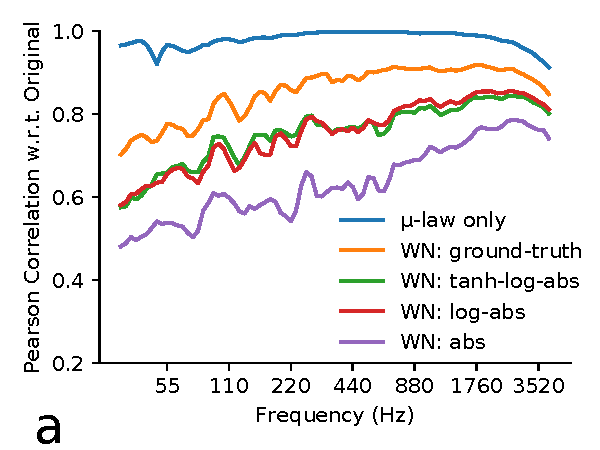
\includegraphics[width=0.5\linewidth]{correlations.pdf}
	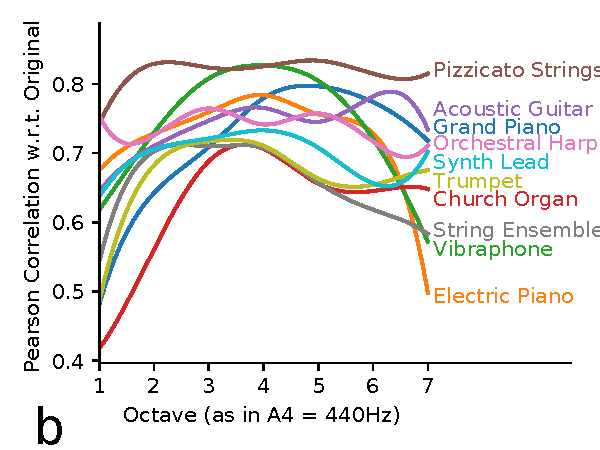
\includegraphics[width=0.5\linewidth]{correlations-instrument.pdf}
	\caption{Pearson correlations between the reconstructed and original audio. (a) each stage of degradation. (b) per-instrument breakdown of the green curve on the left. The curves are smoothed and drawn with respect to each octave for readability.}
	\label{fig:correlations}
	\vspace{-1em}
\end{figure}

\subsubsection{Numerical Analysis of Audio Degradation}

The model goes through several stages of prediction, and each stage incurs a degradation of audio quality.
There necessarily exists some degradation caused by the $\mu$-law quantization, and WaveNet adds additional degradation due to its limited model capacity.
The generated audio is further degraded when imperfect Mel spectrogram predictions are given.
As an objective measure of audio quality degradation at each stage and for each instrument, we plot the Pearson correlations between the synthesized and original audio in Figure \ref{fig:correlations}.
To calculate and visualize the correlations with respect to evenly spaced octaves, we use 84-bin log-magnitude constant-Q transforms with 12 bins per octave starting from C1 ($\approx 32.70 \textrm{Hz}$) and 512-sample steps.
For ideal synthesis, the Pearson correlation should be close to $1$, and lower correlations indicate larger degradation from the original.

Figure \ref{fig:correlations}a shows the correlations for each stage of degradation and for different loss functions used for training the model.
The degradations are more severe in low frequencies in general, where the WaveNet model sees less number of periods of a note within its fixed receptive field length.
The orange curve showing the correlations for WaveNet synthesis using ground-truth Mel spectrograms already exhibits a significant drop from the top curve; this defines an upper bound of Mel2Mel's synthesis quality.
The lower three curves correspond to the loss functions in Equations \ref{eqn:abs-loss}-\ref{eqn:tanh-log-abs-loss}, among which the abs MSE loss clearly performs the worse than the other two which have almost identical Pearson correlation curve, indicating that the MSE loss is more effective in the log-magnitude scale.

Figure \ref{fig:correlations}b shows the breakdown of the curve corresponding to Equation \ref{eqn:tanh-log-abs-loss} into each of the 10 instruments.
There are rather drastic differences among instruments, and most instruments have low Pearson correlations in low pitches except pizzicato strings.
The reasons and implications of these trends are discussed in the following subsection, in comparison with the subjective audio quality test.

\subsubsection{Subjective Audio Quality Test}\label{sec:subjective}

We performed a crowdsourced test asking the listeners to rate the quality of synthesis using a 5-point mean opinion score (MOS) scale with 0.5-point steps.
MOS allows a simple interface that is more suitable for non-expert listeners in a crowdsourcing setup than e.g. MUSHRA \TODO{remove the subjective test part} and is used as a standard approach for assessing the perceptual quality of WaveNet syntheses \cite{oord2016wavenet,oord2018parallel}.
For each of the six configurations corresponding to the curves in Figure \ref{fig:correlations}a in addition to the original audio, the first 20 seconds of the 140 validation tracks are evaluated.
The listeners were provided with a randomly selected segment at a time, and each segment was evaluated by three listeners, comprising 420 samples in each configuration.
18 or less questions were given to each listener, and 173 unique listeners participated.

\begin{table}
	\centering
	\begin{tabular}{l|c} 
		Condition & Mean Opinion Scores \\ \hline
		Original audio & 4.301 $\pm$ 0.080 \\
		$\mu$-law encode-decoded audio & 3.876 $\pm$ 0.097 \\
		WaveNet: ground-truth Mel & 3.383 $\pm$ 0.100 \\
		\hline
		WaveNet: tanh-log-abs MSE & \textbf{3.183 $\pm$ 0.106} \\
		WaveNet: log-abs MSE & 3.019 $\pm$ 0.109 \\
		WaveNet: abs MSE & 2.751 $\pm$ 0.110 \\
	\end{tabular}
	\vspace{1em}
	\caption{\TODO{caption}}\label{tab:synthesis-quality}
\end{table}

This table shows the mean opinion scores (MOS) and the 95\% confidence intervals, which generally follow the tendency similar to Figure \ref{fig:correlations}.
Using the soft-thresholding loss in Equation \ref{eqn:tanh-log-abs-loss} results in the best subjective quality among the three loss functions compared, more significantly so than the numerical comparison in Figure \ref{fig:correlations}.

\setlength{\intextsep}{.1em}
\setlength{\columnsep}{1em}%

\begin{figure}[t]
	\centering
	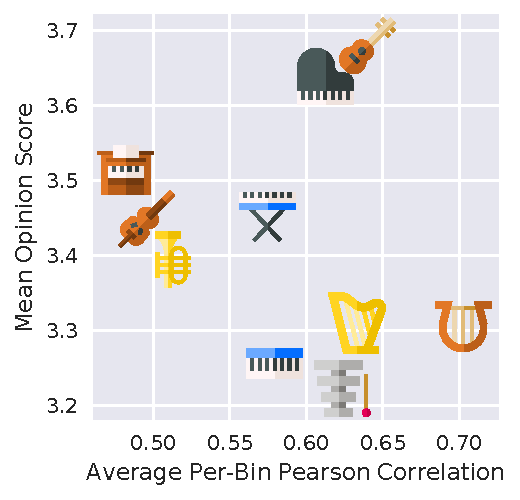
\includegraphics[width=0.4\linewidth]{scatter.pdf}
	\caption{Per-instrument plot of synthesis quality, using the same icons as in Fig. \ref{fig:embedding}.\newline}
	\label{fig:scatter}
	\vspace{-1em}
\end{figure}

In Figure \ref{fig:scatter}, we compare the numerically and perceptually evaluated quality for each instrument.
The horizontal coordinates are the average values for each curve in Figure \ref{fig:correlations}b.
Pearson correlations between CQT are not necessarily indicative of the subjective synthesis quality, because a large contrast in the temporal envelope can contribute to high Pearson correlations, notwithstanding a low perceptual quality.
Reflecting this, more transient instruments in the lower right such as pizzicato strings achieve higher Pearson correlations compared to the MOS, while more sustained instruments on the left side have relatively lower Pearson correlations but have higher perceptual quality.


\subsection{The Timbre Embedding Space}

To make sense of how the learned embedding space conveys timbre information, we construct a 320-by-320 grid that encloses all instrument embeddings and predict the Mel spectrogram conditioned on every pixel in the grid.
The spectral centroid and the mean energy corresponding to each pixel are plotted in Figure \ref{fig:embedding}, which are indicative of the two main aspects of instrumental timbres: the spectral and temporal envelopes.
A higher spectral centroid signifies stronger harmonic partials in high frequency, while a lower spectral centroid indicates that it is closer to a pure sine tone.
Similarly, higher mean energy implies a more sustained tone, and low mean energy means that the note is transient and decays rather quickly.
The points corresponding to the 10 instruments are annotated with instrument icons.\footnote{The icons are made by Freepik and licensed by CC 3.0 BY.}
These plots show that the learned embedding space forms a continuous span over the timbres expressed by all instruments in the training data.
This allows us to use the timbre embedding as a flexible control space for the synthesizer, and timbre morphing is possible by interpolating along curves within the embedding space.

To illustrate how the model scales with more diverse timbre, we train the Mel2Mel model with 100 instruments using a 10-dimensional embedding, and we refer the readers to the web demo$^\textrm{5}$ for an interactive $t$-SNE visualization~\cite{maaten2008tsne} of the embedding space.
The 10-dimensional embedding space also contains a locally continuous timbre distribution of instruments, as in Figure \ref{fig:embedding}, implying that the Mel2Mel model is capable of scaling to hundreds of instruments and to a higher-dimensional embedding space.

In addition to the audio samples used in the experiments, our interactive web demo$^\textrm{1}$ %\footnote{\url{https://neural-music-synthesis.github.io}}
showcases the capability of flexible timbre control, where the Mel2Mel model runs on browser to convert preloaded or user-provided MIDI files into Mel spectrograms using a user-selected point in the embedding space.
% The WaveNet inference requires a custom CUDA kernel and cannot run on browser, so the web demo plays a pre-synthesized version of audio at each point of the embedding space.

\begin{figure}[t]
	\centering
	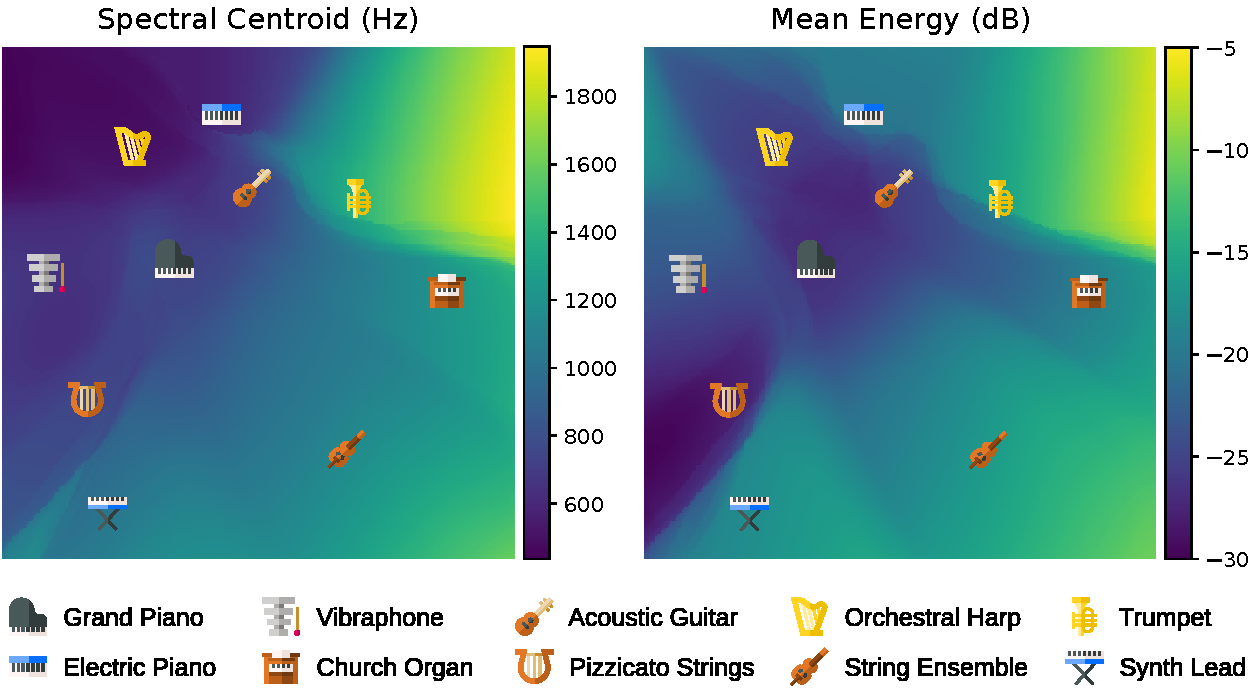
\includegraphics[width=\columnwidth]{runpixels.pdf}
	\caption{Visualization of the embedding space trained in 2 dimensions, using spectral centroids and mean energy. The continuous colors are obtained for each pixel in the 320-by-320 grid and are related to the spectral and temporal envelopes of the timbres.}
	\label{fig:embedding}
	\vspace{-1em}
\end{figure}


\section{Conclusions and Future Directions}\label{sec:conclusions}

We showed that it is possible to build a music synthesis model by combining a recurrent neural network and FiLM conditioning layers, followed by a WaveNet vocoder.
It successfully learns to synthesize musical notes according to the given note sequence and timbre embedding in a continuous timbre space, providing the ability of flexible timbre control for music synthesizers.

The capacity of the WaveNet, such as the number of residual channels and the number of layers, is limited due to the memory requirements of the nv-wavenet implementation, and the degradation from $\mu$-law quantization is also apparent in the experiments.
These limitations can be overcome by Parallel WaveNet \cite{oord2018parallel}, which does not require a special CUDA kernel for fast synthesis and uses a continuous probability distribution for generation, thereby avoiding the quantization noise.
Our earlier experiments on continuous emission failed to stably perform autoregressive sampling due to teacher forcing, and the future work includes investigating this phenomenon comparing with \cite{hawthorne2019maestro}, which used a mixture of logistics distributions to produce high-quality piano sounds.

A notable observation is that the WaveNet vocoder is able to synthesize polyphonic music from Mel spectrograms containing only 80 frequency bins, which are not even aligned to the tuning of the audio files.
While more information available from the increased bins should help synthesize more accurate audio, predicting the higher-dimensional representation becomes more compute-intensive and inaccurate, making 80 bins a sweet spot for use with WaveNet.
Introducing an adversarial loss function for predicting high-resolution images \cite{ledig2017superresolution} can be a viable direction for predicting more accurate and realistic Mel spectrograms for conditioning WaveNet.

Overall, we have demonstrated that a MIDI-to-audio synthesizer can be learned directly from audio, and that this learning allows for flexible timbre control.
Once extended with an improved vocoder and trained on real audio data, we believe the model can result in a powerful and quite realistic music synthesis model.

%!TEX root = ../dissertation.tex
% this file is called up by thesis.tex
% content in this file will be fed into the main document

\graphicspath{{6-adversarial/figures/}}

\chapter{Adversarial Learning for Piano Transcription}
\label{ch:adversarial}

In the previous chapter, we have introduced a WaveNet-based music synthesis model that is conditioned on predicted Mel spectrograms.
A Mel spectrogram is a representation of audio whose dimension is in the order of hundreds at each frame.
Accurate prediction of such high-dimensional representations requires sophisticated modeling of their statistical properties as well as extensive computational power to realize it.
Piano roll representations of music, which are formulated in Chapter \ref{ch:introduction} as the output representation of polyphonic music transcription throughout this thesis, are another example of high-dimensional representations of audio which contain hundreds of data points at each instant.
Therefore, unlike the single-pitch objective in Chapter \ref{ch:monophonic}, prediction of piano roll representations is inherently a multi-label problem and thus warrants a mathematical model that is right for high-dimensional representation.

In this chapter, as hinted in the conclusions in the last chapter, we discuss a method to include adversarial loss to allow the model to predict the piano roll target more accurately.
We first address a limitation in the conventional, element-wise definition of loss functions in which the inter-label probabilistic dependences are not accurately modeled.
Based on this observation, we show that appending an adversarial discriminator to a discriminative piano transcription model can help producing more confident predictions which in turn improve the transcription accuracy.
The content of this chapter is largely based on the work presented at ISMIR 2019 \cite{kim2019adversarial}.


\section{Introduction}

Automatic music transcription (AMT) is a multifaceted problem and comprises a number of subtasks, including multi-pitch estimation (MPE), note tracking, instrument recognition, rhythm analysis, score typesetting, etc.
% Among these, multi-pitch estimation (MPE) is often considered to be the most challenging, as it involves many difficulties such as overlapping harmonics of concurrent pitches, separation of simultaneous sources, and the scarcity of reliable annotations~\cite{benetos2019amt}.
MPE predicts a set of concurrent pitches that are present at each instant, and it is closely related to the task of note tracking, which predicts the onset and offset timings of every note in audio.
In this chapter, we address an issue in the recent approaches for MPE and note tracking, where the probabilistic dependencies between the labels are often overlooked.

\iffalse
\begin{figure}[t]
	\centering
	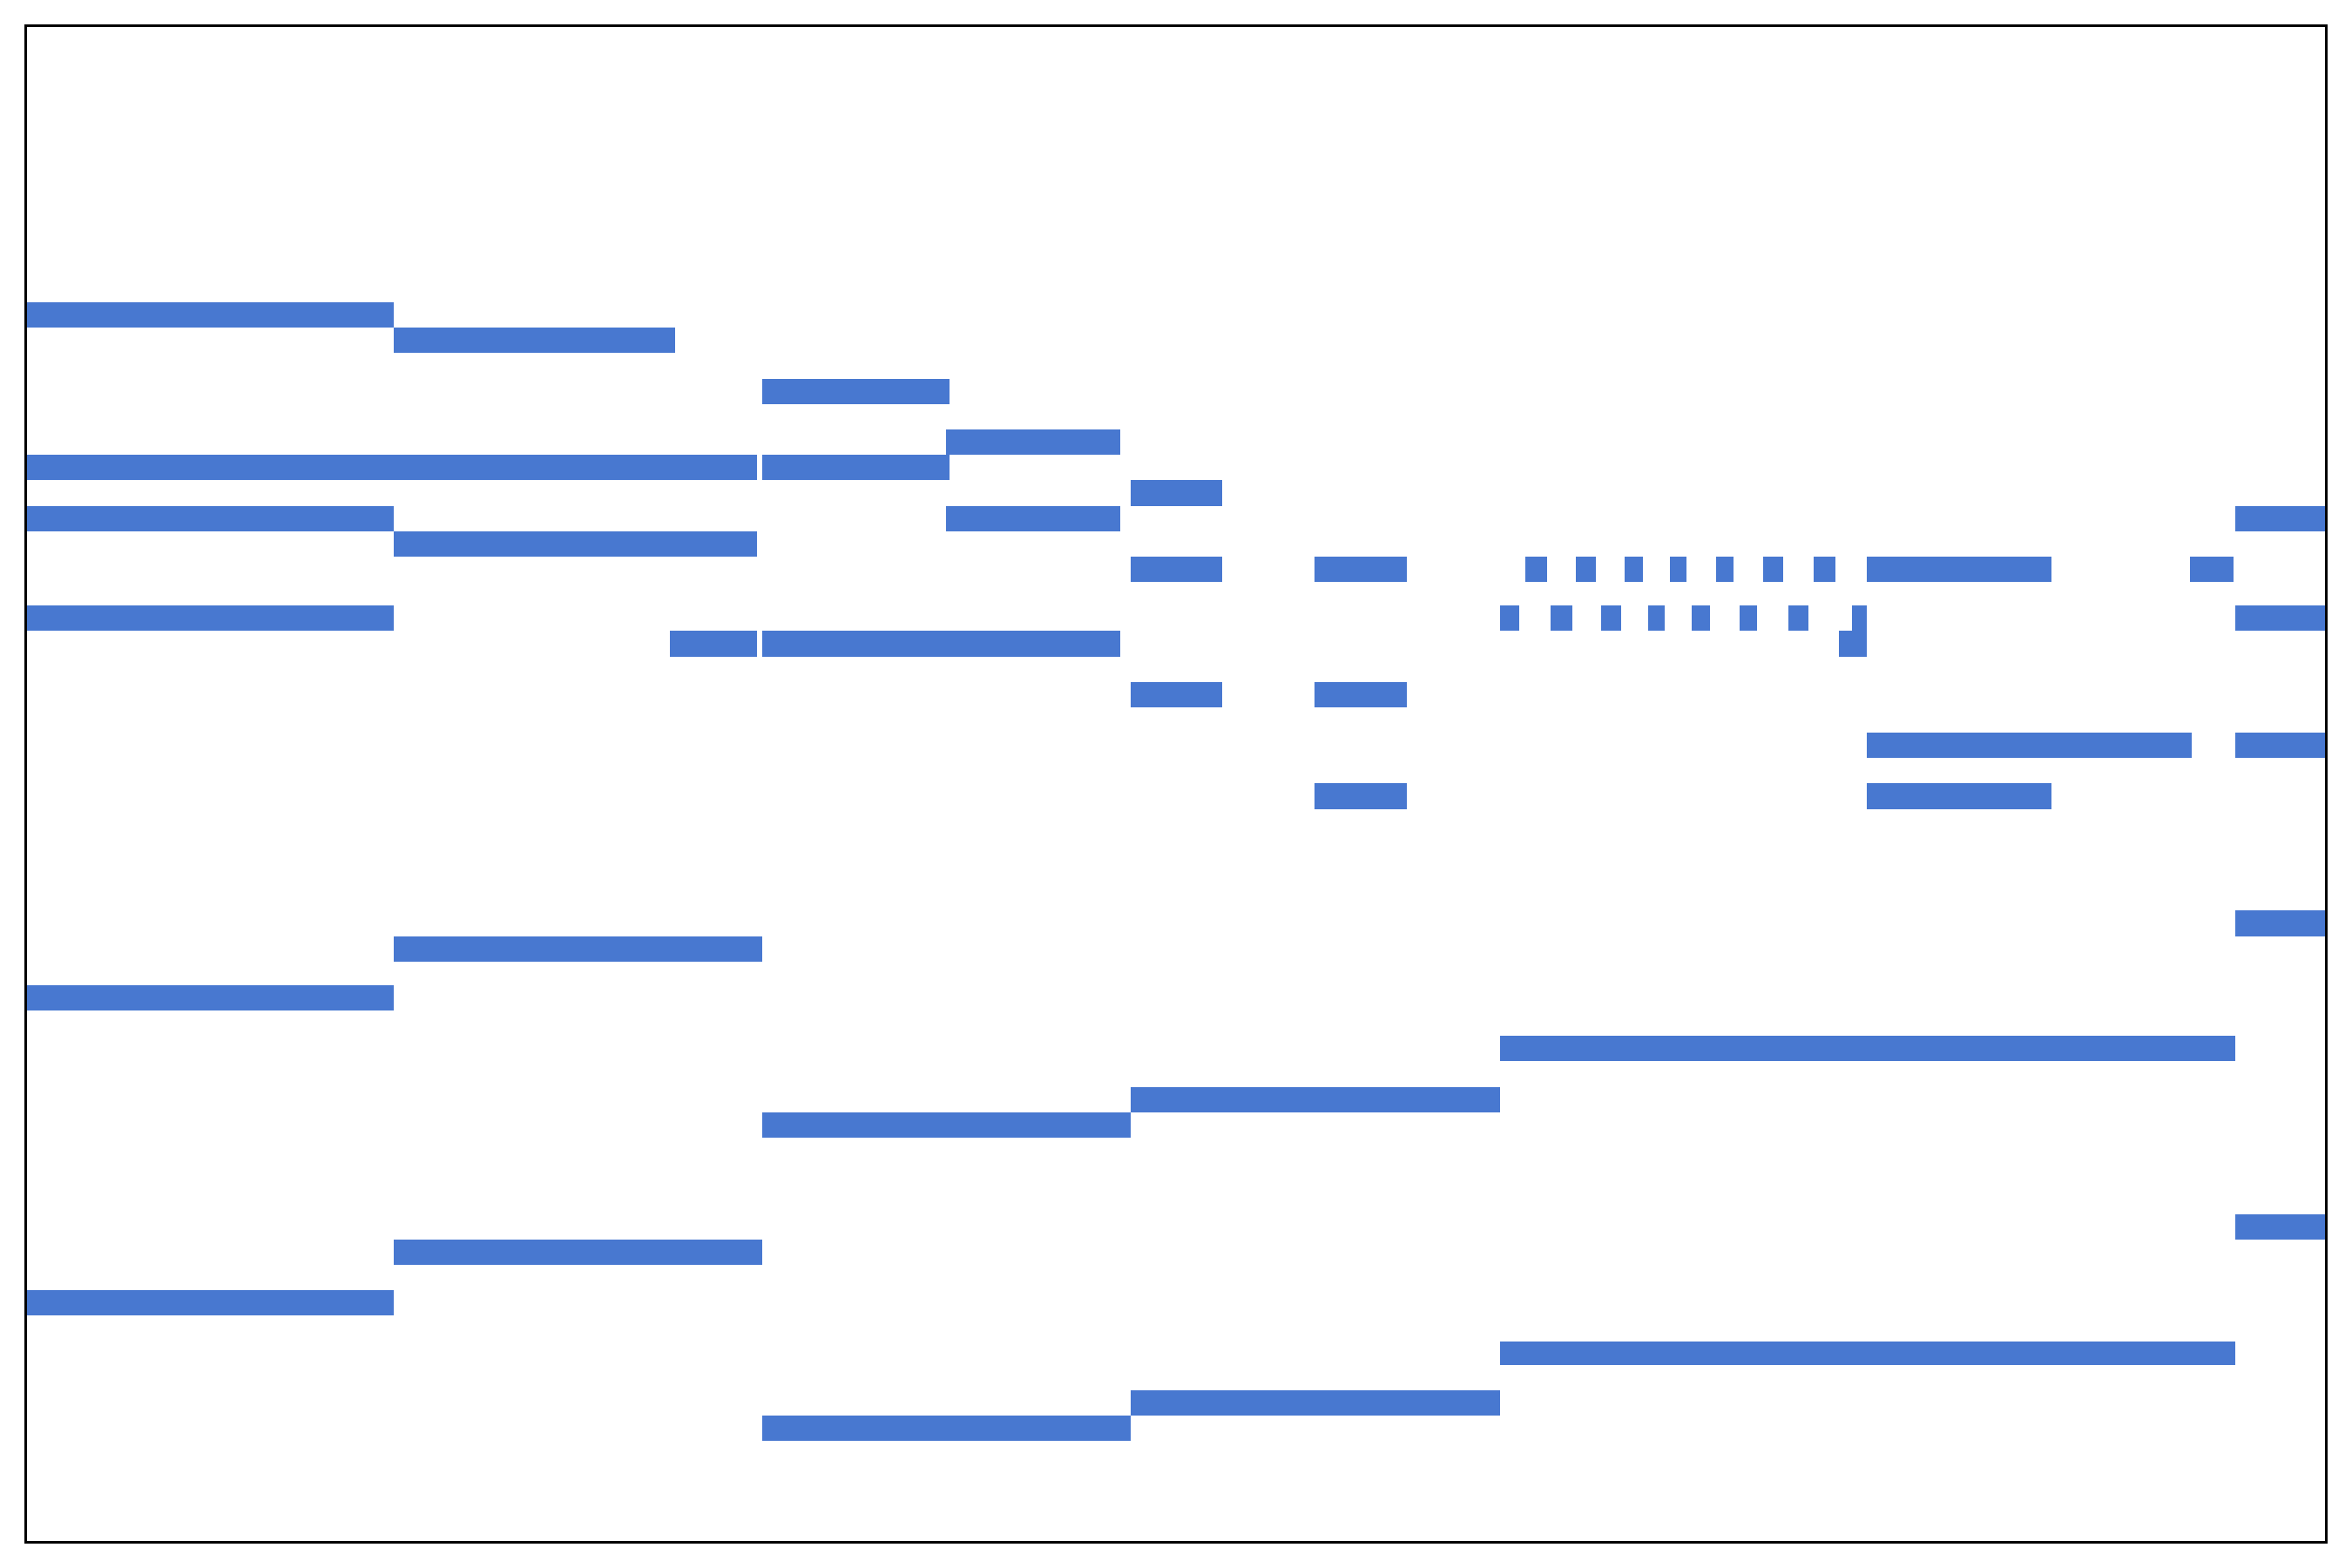
\includegraphics[width=0.49\columnwidth]{pianoroll.pdf}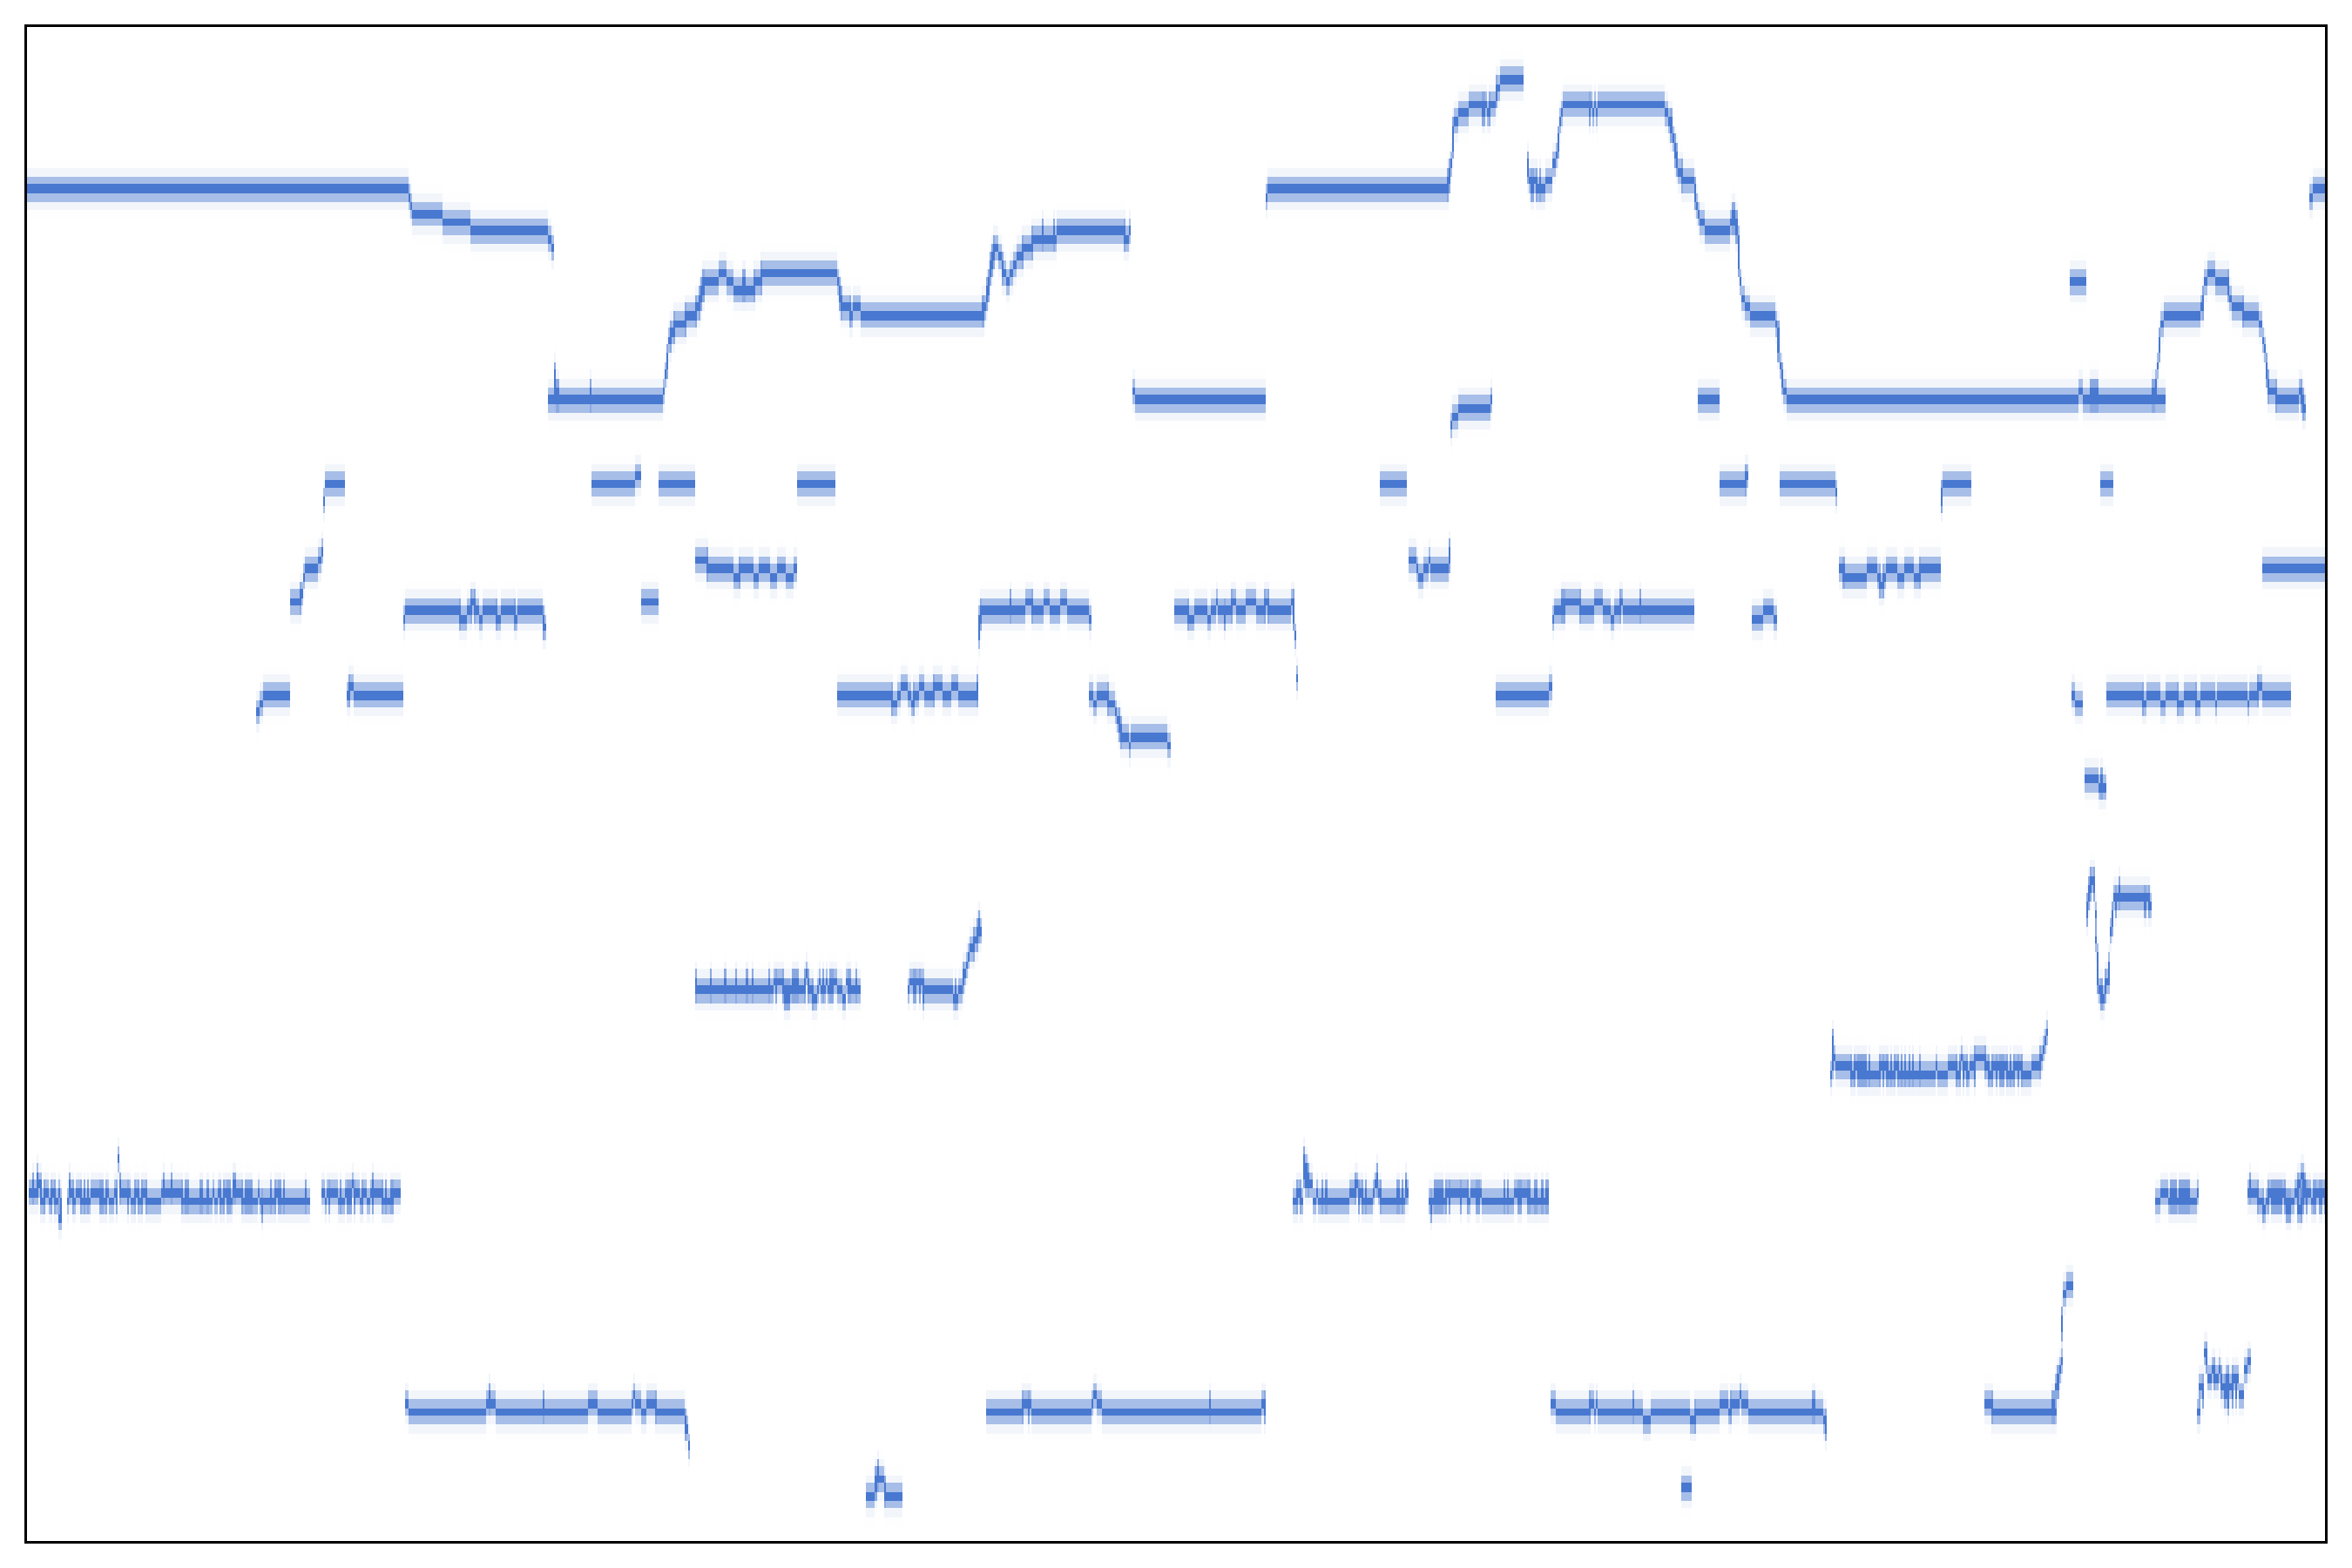
\includegraphics[width=0.49\columnwidth]{deepsalience.pdf}
	\label{fig:2d}
	\caption{Examples of 2-D prediction targets for music transcription: (left) a piano roll, (right) deep salience~\cite{bittner2017deepsalience}.}
\end{figure}
\fi

A common approach for MPE and note tracking is through the prediction of a two-dimensional representation that is defined along the time and frequency axes and contains the pitch tracks of notes over time.
Piano rolls %(Figure~\ref{fig:2d}, left)
are the most common example of such representations, and deep salience~\cite{bittner2017deepsalience} %(Figure~\ref{fig:2d}, right)
is another example that can contain more granular information on pitch contours.
Once such representation is obtained, pitches and notes can be decoded by thresholding~\cite{kelz2016framewise} or other heuristic methods~\cite{kim2018crepe,hawthorne2018onsetsframes}.


To train a model that predicts a two-dimensional target representation $\hat{\Y} \in \R^{P \times T}$ from an input audio representation $\X$, where $P$ is the number of pitch labels and $T$ is the number of time frames, a common approach is to minimize the element-wise sum of a loss function $\mathcal{L}$:
\begin{equation}\label{eqn:elementwise}
\textrm{minimize} ~~ \mathcal{L}(\hat{\Y}, \Y) = \sum_{p=1}^{P}  \sum_{t=1}^{T} \mathcal{L} (\hat{\Y}_{pt}, \Y_{pt}),
\end{equation}
where $\Y \in \mathbb{R}^{P \times T}$ is the ground truth.
In a probabilistic perspective, we can interpret $\mathcal{L}$ as the negative log-likelihood of the model parameters $\vartheta$ of a discriminative model $p_\vartheta(\Y | \X)$:
\begin{equation}
p_\vartheta(\Y | \X) ~=~ e^{\shortminus\mathcal{L}(\hat{\Y}, \Y)} = \prod_{p=1}^{P} \prod_{t=1}^{T} e^{\shortminus\mathcal{L}(\hat{\Y}_{pt}, \Y_{pt})} = \prod_{p=1}^{P} \prod_{t=1}^{T} p_\vartheta(\Y_{pt} | \X)
\end{equation}
which indicates that each element of the label $\Y$ is conditionally independent with each other given the input $\X$.
This encourages the model to predict the average of the posterior, making blurry predictions when the posterior distribution is multimodal, e.g. natural images~\cite{dosovitskiy2016generating}.
%This makes predictions blurry by encouraging the model to predict the average of fast or nuanced events, e.g. trills.

Music data is highly contextual and multimodal, and the conditional independence assumption does not hold in general.
This is why many computational music analysis models employ a separate post-processing stage after sequence prediction.
One approach is to factorize the joint probability using the chain rule and assume the Markov property:
\begin{equation}
p_\vartheta(\Y|\X) \approx \prod_{p=1}^{P} \prod_{t=1}^{T} p_\vartheta(\Y_{pt} | \Y_{\cdot(t-1)}, \X).
\end{equation}
This corresponds to appending hidden Markov models (HMMs) \cite{poliner2006discriminative} or recurrent neural networks (RNNs) \cite{sigtia2016endtoend,hawthorne2018onsetsframes} to the transcription model.
The Markov assumption is effective for one-dimensional sequence prediction tasks, such as chord estimation~\cite{ni2012harmonic} and monophonic pitch tracking~\cite{mauch2014pyin}, but when predicting a two-dimensional representation, it still does not address the inter-label dependencies along the frequency axis.


There exist a number of models in the computer vision literature that can express inter-label dependencies in two-dimensional predictions, such as the neural autoregressive distribution estimator (NADE)~\cite{larochelle2011nade}, PixelRNN~\cite{oord2016pixelrnn}, and PixelCNN~\cite{oord2016pixelcnn}.
However, apart from a notable exception using a hybrid RNN-NADE approach~\cite{boulangerlewandowski2012temporal}, the effect of learning the joint posterior distribution for polyphonic music transcription has not been well studied.


To this end, we propose a new approach for effectively leveraging inter-label dependencies in polyphonic music transcription. We pose the problem as an image translation task and apply an adversarial loss incurred by a discriminator network attached to the baseline model.
We show that our approach can consistently and significantly reduce the transcription errors in \emph{Onsets and Frames} \cite{hawthorne2018onsetsframes}, a state-of-the-art music transcription model.


\section{Background}

\subsection{Automatic Transcription of Polyphonic Music}

Automatic transcription models for polyphonic music can be classified into frame- or note-level approaches.
Frame-level transcription is synonymous with multi-pitch estimation (MPE) and operates on tiny temporal slices of audio, or frames, to predict all pitch values present in each frame.
%Multi-pitch estimation (MPE) and multi-F0 estimation are synonymous with frame-level transcription.
Note-level transcription, or note tracking, operates at a higher level, predicting a sequence of note events that contains the pitch, the onset time, and optionally the offset time of each note.
Note tracking is typically implemented as a post-processing stage on the output of MPE~\cite{benetos2019amt}, by connecting and grouping the pitch estimates over time to produce discrete note events.
In this sense, we can say that MPE is at the core of polyphonic music transcription.

Among the approaches for MPE reviewed in Section \ref{ch:mir}.\ref{sec:mffe}, two categories have been most successful in recent years: matrix factorization \cite{lee2001nmf} and deep learning \cite{lecun2015deeplearning}.
Commonly in both of these approaches, an iterative gradient-descent algorithm is used to minimize an element-wise loss function that is defined on two-dimensional representation.
NMF-based methods are designed to minimize a divergence function between the matrix factorization and the target matrix, and similarly in deep learning models, neural networks are optimized to predict a two-dimensional representation that makes an element-wise loss function as small as possible.


In this chapter, we use Onsets and Frames~\cite{hawthorne2018onsetsframes}, a state-of-the-art piano transcription model based on deep learning, as our baseline.
It uses multiple columns of convolutional and recurrent neural network layers to predict onsets, offsets, velocities, and frame labels from the Mel spectrogram input, as shown in Figure~\ref{fig:onsetsframes}.
Predicted onset and frame posteriors are then used for decoding the note sequences, where a threshold value is used to create binary onset and frame activations, and frame activations without the corresponding onsets are disregarded.
Onsets and Frames also uses an element-wise optimization objective which does not consider the inter-label dependencies.
This motivates the adversarial training scheme that is outlined in the following subsection.


\begin{figure}[t]
	\centering
	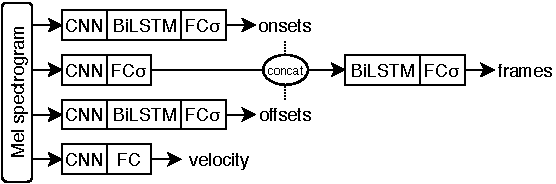
\includegraphics[width=0.8\columnwidth]{onsetsframes.pdf}
	\caption{The Onset and Frames model. CNN denotes the convolutional acoustic model taken from~\protect\cite{kelz2016framewise}, FC denotes a fully connected layer, and $\sigma$ denotes sigmoid activation. Dotted lines mean stop-gradient, i.e. no backpropagation.}
	\label{fig:onsetsframes}
\end{figure}


\subsection{Generative Adversarial Networks and \texttt{pix2pix}}

As extensively reviewed in Section \ref{ch:deeplearning}.\ref{sec:gan}, generative adversarial networks (GANs)~\cite{goodfellow2014gan} refer to a family of deep generative models which consist of two components, namely the generator $G$ and the discriminator $D$.
Given a data distribution $\x \sim p(\x)$ and latent codes $\z \sim p(\z)$, GAN performs the following minimax game:
\begin{equation}\label{eqn:gan}
\min_{G} \max_{D}  \underbrace{\Big [ \E_{\x} \log D(\x) + \E_{\z} \log (1 - D ( G(\z))) \Big ]}_{\mathcal{L}_{\text{GAN}}(G, D)}.
\end{equation}
$G$ and $D$ are implemented as neural networks trained in an adversarial manner, where the discriminator learns to distinguish the generated samples from the real data, while the generator learns to produce realistic samples to fool the discriminator.
GANs are most renowned for their ability to produce photorealistic images~\cite{karras2019stylegan} and have shown promising results on music generation as well~\cite{engel2019gansynth,dong2018musegan,yang2017midinet}.
We refer the readers to~\cite{goodfellow2016gan,creswell2017gan} for a comprehensive review of the techniques, variants, and applications of GANs.

The second term in Equation~\ref{eqn:gan} has near-zero gradients when $D(G(\z)) \approx 0$, which is usually the case in early training.
To avoid this, a \textit{non-saturating} variant of GAN is suggested in~\cite{goodfellow2014gan} where the generator is trained with the following optimization objective instead:
\begin{equation}\label{eqn:nsgan}
\max_{G}~ \E_{\z} \log D(G(\z)).
\end{equation}
The non-saturating GAN loss is used more often than the minimax loss in Equation \ref{eqn:gan} and is implemented by flipping the labels of fake data while using the same loss function.
\textit{Least-squares GAN} \cite{mao2017lsgan} is an alternative method to address the vanishing gradient problem, which replaces the cross entropy loss in Equations \ref{eqn:gan}-\ref{eqn:nsgan} with squared errors:%
\begin{equation}\label{eqn:lsgan}
	\begin{array}{l@{}l}
	\displaystyle\min_{D} ~\Big [ \E_{\x} (D(\x) - 1)^2 + \E_{\z} D(G(\x))^2 \Big ], \\
	\displaystyle\min_{G} ~\>\E_{\z} (D(G(\z)) - 1)^2.
	\end{array}
\end{equation}
The non-saturating GAN (NSGAN) and least-squares GAN (LSGAN) losses are examples of GAN losses that define the objective used during the minimax optimization, and we will use these two losses in conjunction with the conditional GAN setup described below.

While the default formulation of GAN concerns unconditional generation of samples from $p(\mathbf{x})$, conditional GANs (cGAN)~\cite{mirza2014conditional} produce samples from a conditional distribution $p(\y|\x)$. To do this, the generator and the discriminator are defined in terms of                                                                                                                                                                                                                                                     the condition variable $\x$ as well:
\begin{equation}
\label{eqn:cgan}
\min_{G}\max_{D}\underbrace{\Big [ \mathbb{E}_{\x,\y} \log D(\x,~\y) + \mathbb{E}_{\x,\z} \log (1 - D ( \x,~ G(\x,~\z)) \Big ]}_{\mathcal{L}_{\text{cGAN}}(G, D)}.
\end{equation}
\texttt{pix2pix} \cite{isola2017pix2pix} is an image translation model that learns a mapping between two distinct domains of images, such as aerial photos and maps.
A \texttt{pix2pix} model takes paired images $(\x, \y)$ as its training data and minimizes the conditional GAN loss along with an additional L1 loss:
\begin{equation}\label{eqn:l1}
\mathbb{E}_{\mathbf{x},\mathbf{y},\mathbf{z}} ~ \big \lVert ~ \y - G(\x, \z) ~ \big \rVert_1,
\end{equation}
which encourages the conditional generator to learn the forward mapping from $\mathbf{x}$ to $\mathbf{y}$. It can be thought that the GAN loss in Equation \ref{eqn:cgan} is fine-tuning the mapping learned by the L1 loss in Equation \ref{eqn:l1}, resulting in a predictive mapping that better respects the probabilistic dependencies within the labels $\y$.

We adapt this approach to music transcription tasks and show that we can indeed improve the performance by introducing an adversarial loss to an existing music transcription model.



\section{Method}

We describe a general method for improving an NN-based transcription model $G$ that performs prediction of a two-dimensional target $\Y$ from an input audio representation $\X$.
Say the original model $G$ is trained by minimizing the loss $\mathcal{L}_{\textrm{task}}(G(\X), \Y)$ between the predicted target $\hat{\Y} = G(\X)$ and the ground-truth $\Y$. 
The main idea of our method is to adapt \texttt{pix2pix}~\cite{isola2017pix2pix} to this setup, by introducing an adversarial discriminator $D$ during the training process.
The adversarial training objective includes the conditional GAN loss $\mathcal{L}_{\text{cGAN}}$ (Equation \ref{eqn:cgan}):
\begin{equation}
\min_{G}\max_{D} \E_{\X,\Y} \Big [ \nu\mathcal{L}_{\text{task}} (G(\X), \Y) + \mathcal{L}_{\text{cGAN}}(G, D) \Big ],
\end{equation}
where $\nu$ is a hyperparameter that controls how much the conditional GAN loss contributes to the gradient steps relative to the discriminative loss $\mathcal{L}_{\text{task}}$.
Figure \ref{fig:discriminator} illustrates how the two components are connected in the computation graph and how the loss terms are calculated.

\begin{figure}[t]
	\centering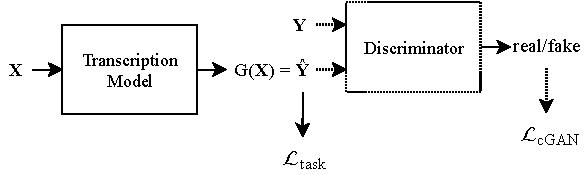
\includegraphics[width=0.8\columnwidth]{discriminator.pdf}
	\caption{A computation graph showing how a discriminator is appended to the original model. The appended parts are shown as dotted components.}\label{fig:discriminator}
\end{figure}

Adversarial training with $\mathcal{L}_{\text{cGAN}}$ allows the model to learn the inter-label dependencies as desired, even when $\mathcal{L}_{\text{task}}$ is defined only in terms of element-wise operations between $\hat{\Y}$ and $\Y$, as in Equation \ref{eqn:elementwise}.
In the next subsection, we describe a neural network architecture for the  cGAN discriminator that leverages prior knowledge on music.


\subsection{Musically Inspired Adversarial Discriminator}

Following \texttt{pix2pix}, we use a fully convolutional architecture~\cite{long2015fcn} for the discriminator.
By being fully convolutional, the discriminator has translation invariance not only along the time axis (as in HMMs and RNNs) but also along the frequency axis.
Since the discriminator determines how realistic a polyphonic note sequence is, the translation invariance enforces that the decision does not depend on the musical key, but only on the relative pitch and time intervals between the notes.
This effectively implements a music language model (MLM)~\cite{boulangerlewandowski2012temporal,sigtia2016endtoend} and biases the transcription toward more realistic note sequences.

Unlike the image-to-image translation problem, the input representations (e.g.~Mel spectrograms) and the output representations (e.g.~piano rolls) of a music transcription model can have different dimensions.
This makes combining $\X$ and $\Y$ in a fully convolutional manner difficult.
For this reason, we make the discriminator a function of $\Y$ only, simplifying the objective in Equation \ref{eqn:cgan} to:
\begin{equation}\label{eqn:simple-cgan}
\mathcal{L}_{\text{cGAN}}(G, D) ~ = ~  \mathbb{E}_{\Y}  \log D(\Y) ~ + ~ \mathbb{E}_{\X} \log (1 - D ( G(\X))).
\end{equation}
Note that $\z$ is also omitted in Equation \ref{eqn:simple-cgan}, as we follow \cite{isola2017pix2pix} and implement the stochasticity of $\z$ only in terms of dropout layers \cite{srivastava2014dropout}, without explicitly feeding random noises into the generator.
This causes a mode collapse problem where the learned $p(\Y|\X)$ is not diverse enough, but it does not harm our purpose of producing more realistic target representations.

\subsection{TTUR and \textit{mixup} to Stabilize GAN Training}

Although an ideal GAN generator can fully reconstruct the data distribution at the global optimum~\cite{goodfellow2014gan}, training of GANs in practice is notoriously difficult, especially for high-dimensional data~\cite{goodfellow2016gan}.
This led to the inventions of a plethora of techniques for stabilizing GAN training, among which we employ the two-timescale update rule (TTUR)~\cite{heusel2017ttur} and \textit{mixup}~\cite{zhang2018mixup}.
TTUR means simply setting the generator's learning rate a few times larger than that of the discriminator, which has been empirically shown to stabilize GAN training significantly.

The other technique, \textit{mixup}, is an extension to empirical risk minimization where training data samples are drawn from convex interpolations between pairs of empirical data samples.
For a pair of feature-target tuples $(\X_i, \Y_i)$ and $(\X_j, \Y_j)$ sampled randomly from the empirical distribution, their convex interpolation is given by:
\begin{equation}
\begin{array}{l@{}l}
\tilde{\X} = \lambda \X_i + (1 - \lambda) \X_j \\
\tilde{\Y} = \lambda \Y_i + (1 - \lambda) \Y_j
\end{array}
\end{equation}
where $\lambda \sim \text{Beta}(\alpha, \alpha)$, and $\alpha$ is the \textit{mixup} hyperparameter which controls the strength of interpolation.
When $\alpha = 0$, the Beta distribution becomes $\text{Bernoulli}(0.5)$ which recovers the usual GAN training without \textit{mixup}.



\setlength{\algomargin}{0em}
\DontPrintSemicolon
\SetInd{0.1em}{2em}
\begin{algorithm2e}[b!]
	\vspace{-0.3em}\noindent
	\caption{Training of a \textit{mixup} Conditional GAN.}\label{alg:training}
	\setstretch{1.05}
	\rule{\columnwidth}{0.75pt}\\
	\KwIn{
		Generator $G_\vartheta(\X)$ with initial parameters $\vartheta$, learning rate $\eta$, and loss function $\mathcal{L}_{\text{task}}(\hat{\Y}, \Y)$, discriminator $D_\varphi(\Y)$ with initial parameters $\varphi$, learning rate $\beta$, and loss function $\ell \in \{\text{BCE}, \text{MSE}\}$, batch size $m$, training data distribution $p(\X, \Y)$,  \texttt{pix2pix} weight $\nu$, \textit{mixup} strength $\alpha$.
	}

	\KwOut{Trained conditional generator $G_\vartheta(\X)$.}
	\vspace{-0.5em}\noindent
	\rule{\columnwidth}{0.5pt}\\
	%\vspace{-1em}
	\While{$\varphi$ and $\vartheta$ have not converged}{
		$\{(\X_i, \Y_i)\}_{i=1,\cdots,m} \leftarrow m \text{ samples from } p(\X, \Y)$\;
		\For{$i = 1, \cdots, m$}{
			$\hat{\Y}_i \leftarrow G_\vartheta(\X_i)$\;
			$\lambda_i \leftarrow \text{sample from Beta}(\alpha, \alpha)$\;
			$\tilde{\Y}_i \leftarrow \lambda_i \Y_i + (1 - \lambda_i) \hat{\Y}_i$
		}
		$\mathcal{L}_{\text{cGAN}}^D\>\leftarrow \textstyle\sum_{i=1}^M \ell(D_\varphi(\tilde{\Y}_i), \lambda_i)$\;
		$\varphi \leftarrow \varphi - \beta \cdot \nabla_\varphi \mathcal{L}_{\text{cGAN}}^D $\;
		$\mathcal{L}_{\text{cGAN}}^G \leftarrow \textstyle\sum_{i=1}^M \ell (D_\varphi(\tilde{\Y}_i), 1 - \lambda_i) $\;
		$\vartheta \leftarrow \vartheta - \eta \cdot \textstyle\nabla_\vartheta \Big [ \sum_{i=1}^m \nu \mathcal{L}_{\text{task}}(\hat{\Y}_i, Y_i) - \mathcal{L}_{\text{cGAN}}^G \Big ] $
	}
	\vspace{-0.5em}\noindent
	\rule{\columnwidth}{0.75pt}\;
\end{algorithm2e}



\textit{mixup} is readily applicable to the binary classification task of GAN discriminators.
In our conditional GAN setup, we have an additional advantage of having paired samples of a real label $\Y$ and a fake label $\hat{\Y} = G(\X)$, which allow us to replace Equation \ref{eqn:simple-cgan} with:
\begin{equation}\label{eqn:mixup-gan}
\min_{G} ~ \max_{D} ~ \mathbb{E}_{\X,\Y,\lambda} \Big [ - \ell (D(\lambda \Y + (1 - \lambda) G(\X) ), ~ \lambda) \Big ].
\end{equation}
where $\ell(p, y) = - y \log p - (1-y) \log (1-p)$ is the binary cross entropy (BCE) function.
With this \textit{mixup} setup, the discriminator now has to operate on the convex interpolation between the predicted representation and the corresponding ground truth.
This makes the discriminator's task even more difficult when the prediction gets close to the ground truth, which is desirable because the discriminator should be inconclusive (i.e. $D = \tfrac{1}{2}$ everywhere) at the global optimum~\cite{goodfellow2014gan}.

Algorithm \ref{alg:training} details the procedure of training the conditional GAN using \textit{mixup}, based on Equations \ref{eqn:simple-cgan} and \ref{eqn:mixup-gan}.
Note that for training the generator network, we perform label flipping in $\mathcal{L}_{\text{cGAN}}^G$ similarly as in Equation \ref{eqn:nsgan}.
Also, to train a least-squares GAN (Equation \ref{eqn:lsgan}) instead, we can simply replace $\ell$ with a mean squared error (MSE) loss.


\begin{table}[t]
	\small
	\renewcommand\arraystretch{1.2}
	\renewcommand{\tabcolsep}{5pt}
	\centering
	\begin{tabular}{l c} \toprule
		Hyperparameter & Values \\ \hline
		Generator learning rate $\eta$ & 0.0006 \\ 
		Discriminator learning rate $\beta$ & 0.0001 \\
		Discriminator loss function $\ell$ & \{BCE, MSE\}\\
		Batch size $m$ & 8 \\
		\texttt{pix2pix} weight $\nu$ & 100 \\
		\textit{mixup} strength $\alpha$ & \{0, 0.2, 0.3, 0.4\} \\
		Activation threshold $\tau$ & 0.5 \\
		Training sequence length & 327,680 \\
		\bottomrule
	\end{tabular}
	\vspace{1em}
	\caption{Hyperparameters used during the experiments.}\label{tab:hyperparameters}
\end{table}

\begin{table}[t]
	\small
	\centering
	\renewcommand\arraystretch{1.5}
	\renewcommand{\tabcolsep}{0em}
	\newcolumntype{M}[1]{>{\centering\arraybackslash}b{#1}}
	\newcolumntype{C}{>{\centering\arraybackslash}m{2.4em}}
	\begin{tabular}{@{\extracolsep{1em}}lM{4em}M{8em}CCCC}
		& & & \multicolumn{4}{c}{\textit{mixup} strength $\alpha$} \\ \cline{4-7}
		& Baseline & GAN type & 0 & 0.2 & 0.3 & 0.4 \\ \hline
		\multirow{2.25}{5em}{Frame F1} & \multirow{2.25}{4em}{\centering0.899} & Non-Saturating & 0.664 & 0.912 & \textbf{0.914} & 0.907 \\
		& & Least-Squares & 0.904 & 0.903 & 0.906 & 0.898 \\ \hline
		\multirow{2.25}{5em}{Note F1} & \multirow{2.25}{4em}{\centering0.942} & Non-Saturating & 0.717 & 0.953 & \textbf{0.956} & 0.951 \\
		& & Least-Squares & 0.944 & 0.947 & 0.950 & 0.943 \\
		\hline
	\end{tabular}
	\vspace{1em}
	\caption{Frame and note F1 scores are the highest when the non-saturating GAN loss and $\alpha = 0.3$ are used.}\label{tab:alpha}
\end{table}

\begin{table*}[t]
	\centering
	\footnotesize
	\renewcommand\arraystretch{1.5}
	\renewcommand{\tabcolsep}{0em}
	\newcolumntype{M}[1]{>{\centering\arraybackslash}b{#1}}
	\newcolumntype{C}{>{\centering\arraybackslash}m{4em}}
	\begin{tabular}{@{\extracolsep{0.5em}}llllCCCCCCC}
		& & & &\multirow{3.3}{4em}{\centering Baseline} &\multicolumn{3}{M{13em}}{\centering Non-Saturating GAN}
		&\multicolumn{3}{M{13em}}{\centering Least-Squares GAN} \\
		\cline{6-8} \cline{9-11}
		& & & & & $\alpha = 0.2$ & $\alpha = 0.3$ & $\alpha = 0.4$ & $\alpha = 0.2$ & $\alpha = 0.3$ & $\alpha = 0.4$ \\ \hline
		\parbox[t]{2mm}{\multirow{7.4}{*}{\rotatebox[origin=c]{90}{Frame Metrics}}} & & & F1 & 0.899 & 0.912 & \textbf{\small0.914} & 0.907 & 0.901 & 0.906 & 0.898 \\
		& & & Precision ~~~ & 0.946 & 0.937 & 0.931 & 0.939 & 0.940 & 0.942 & 0.946 \\
		& & & Recall & 0.857 & 0.889 & 0.898 & 0.879 & 0.865 & 0.875 & 0.855 \\
		& & & $E_\text{total}$ & 0.179 & 0.157 & 0.156 & 0.166 & 0.176 & 0.167 & 0.181 \\
		& & & $E_\text{subs}$ & 0.013 & 0.013 & 0.012 & 0.013 & 0.014 & 0.013 & 0.013 \\
		& & & $E_\text{miss}$ & 0.130 & 0.097 & 0.089 & 0.108 & 0.121 & 0.113 & 0.132 \\
		& & & $E_\text{fa}$ & 0.036 & 0.047 & 0.054 & 0.045 & 0.042 & 0.042 & 0.036 \\ \hline
		\parbox[t]{2mm}{\multirow{3.2}{*}{\rotatebox[origin=c]{90}{Note}}} & & & F1 & 0.942 & 0.953 & \textbf{\small0.956} & 0.951 & 0.944 & 0.950 & 0.941 \\
		& & & Precision & 0.990 & 0.974 & 0.981 & 0.973 & 0.986 & 0.988 & 0.989 \\
		& & & Recall & 0.899 & 0.933 & 0.932 & 0.930 & 0.905 & 0.916 & 0.898 \\ \hline
		\parbox[t]{2mm}{\multirow{3.2}{*}{\rotatebox[origin=c]{90}{Note with}}} & \parbox[t]{2mm}{\multirow{3.2}{*}{\rotatebox[origin=c]{90}{Offsets}}} & & F1 & 0.802 & 0.811 & \textbf{\small0.813} & 0.799 & 0.799 & 0.810 & 0.798 \\
		& & & Precision & 0.842 & 0.828 & 0.835 & 0.817 & 0.835 & 0.841 & 0.838 \\
		& & & Recall & 0.765 & 0.794 & 0.793 & 0.782 & 0.767 & 0.781 & 0.762 \\ \hline
		\parbox[t]{2mm}{\multirow{3.2}{*}{\rotatebox[origin=c]{90}{Note with}}} & \parbox[t]{2mm}{\multirow{3.2}{*}{\rotatebox[origin=c]{90}{Offsets and}}} & \parbox[t]{4mm}{\multirow{3.2}{*}{\rotatebox[origin=c]{90}{Velocity}}} & F1 & 0.790 & 0.799 & \textbf{\small0.802} & 0.787 & 0.788 & 0.799 & 0.787 \\
		& & & Precision & 0.830 & 0.816 & 0.823 & 0.805 & 0.823 & 0.830 & 0.827 \\
		& & & Recall & 0.755 & 0.783 & 0.782 & 0.770 & 0.757 & 0.771 & 0.752 \\ \hline
	\end{tabular}
	\vspace{1em}
	\caption{Summary of transcription performance. The non-saturating GAN loss achieves the best performance across all F1 metrics. The average metrics across the tracks in the MAESTRO test dataset are reported, and the model checkpoint where the average of frame F1 and note F1 is the highest on the validation dataset is used.}\label{tab:performance}
\end{table*}


\section{Experimental Setup}

To verify the effectiveness of our approach, we compare Onsets and Frames~\cite{hawthorne2018onsetsframes}, a state-of-the-art piano transcription model, with variants of the same model that are trained with the adversarial loss.
We also aim to evaluate the choices of the GAN loss and the \textit{mixup} strength $\alpha$.

\subsection{Model Architecture}

We use the extended Onsets and Frames model~\cite{hawthorne2019maestro} which increased the CNN channels to 48/48/96, the LSTM units to 256, and the FC units to 768.
The extended model has a total of 26.5 million parameters.
We do not use the frame loss weights described in~\cite{hawthorne2018onsetsframes} in favor of the offset stack introduced in the extended version (see Figure~\ref{fig:onsetsframes}).
During inference, we first calculate the posteriors corresponding to overlapping chunks of audio, with the same length as the training sequences, and perform overlap-add (OLA) using Hamming windows to obtain the full-length posterior.
We perform OLA instead of applying the recurrent calculations for the full length, because the effects of adversarial learning are best achieved within the training sequence length.

The input to the discriminator has two channels for the onset and frame predictions.
The discriminator has 5 convolutional layers: \texttt{c32k3s2p1}, \texttt{c64k3s2p1}, \texttt{c128k3s2p1}, \texttt{c256k3s2p1}, \texttt{c1k5s1p2}, where the numbers indicate the number of output channels, the kernel size, the stride amount, and the padding size.
At each non-final layer, dropout of probability 0.5 and leaky ReLU activation with negative slope 0.2 are used.
The mean of the final layer output along the time and frequency axes is taken as the discriminator output.



\subsection{Hyperparameters}

Table \ref{tab:hyperparameters} summarizes the hyperparameters used during the experiments, which are mostly taken directly from~\citeA{hawthorne2018onsetsframes} and \citeA{isola2017pix2pix}.
Also following~\citeA{hawthorne2018onsetsframes}, we use Adam~\cite{kingma2015adam} and apply learning rate decay of factor 0.98 in every 10,000 iterations, for both the generator and the discriminator.
We examine two types of GAN losses, the non-saturating GAN ($\ell = \text{BCE}$) and the least-squares GAN ($\ell = \text{MSE}$).
For each GAN loss, multiple values of \textit{mixup} strengths are compared with $\alpha = 0$, i.e. no \textit{mixup}.
Training runs for one million iterations, and the iteration that best performs on the validation set are used for evaluation on the test set.

\subsection{Dataset}

We use the MAESTRO dataset~\cite{hawthorne2019maestro}, which contains Disklavier recordings of 1,184 classical piano performances.
The dataset consists of 172.3 hours of audio, which are provided with 140.1, 15.3, and 16.9 hours of train/validation/test splits such that recordings of one composition only appear in the same split.
We resample the audio to 16 kHz and down-mix into a single channel.
Following~\citeA{hawthorne2018onsetsframes}, an STFT window of 2,048 samples is used for producing 229-bin Mel spectrograms, and a hop length of 32 ms is used.
% We do not perform audio amplitude normalization on the dataset, following the official implementation.
Training sequences sliced at random positions are used, unlike the official implementation which slices training sequences at silence or zero crossings.

\subsection{Evaluation Metrics}

The Onsets and Frames model perform both frame-level and note-level predictions, and their performance can be evaluated with the standard precision, recall, and F1 metrics.
For multi-pitch estimation, we also report the error rate metrics defined by~\citeA{poliner2006discriminative}, which include total error, substitution error, miss error, and false alarm error.
We use the \texttt{mir\_eval}~\cite{raffel2014mir_eval} library for all metric calculations.
For the note-level metrics, we use the default settings of the library, which use 50 ms for the onset tolerance, 50 ms or 20\% of the note length (whichever is longer) for the offset tolerance, and 0.1 for the velocity tolerance.


\section{Results}

%Our results show that adversarial learning brings a consistent improvement over the baseline which is already very robust, as shown with quantitative and qualitative analyses in the following subsections.


\subsection{Comparison with the Baseline Metrics}

\begin{figure*}[t]
	\centering
	\minipage{1.03\textwidth}
	\hspace{-0.02\textwidth}
	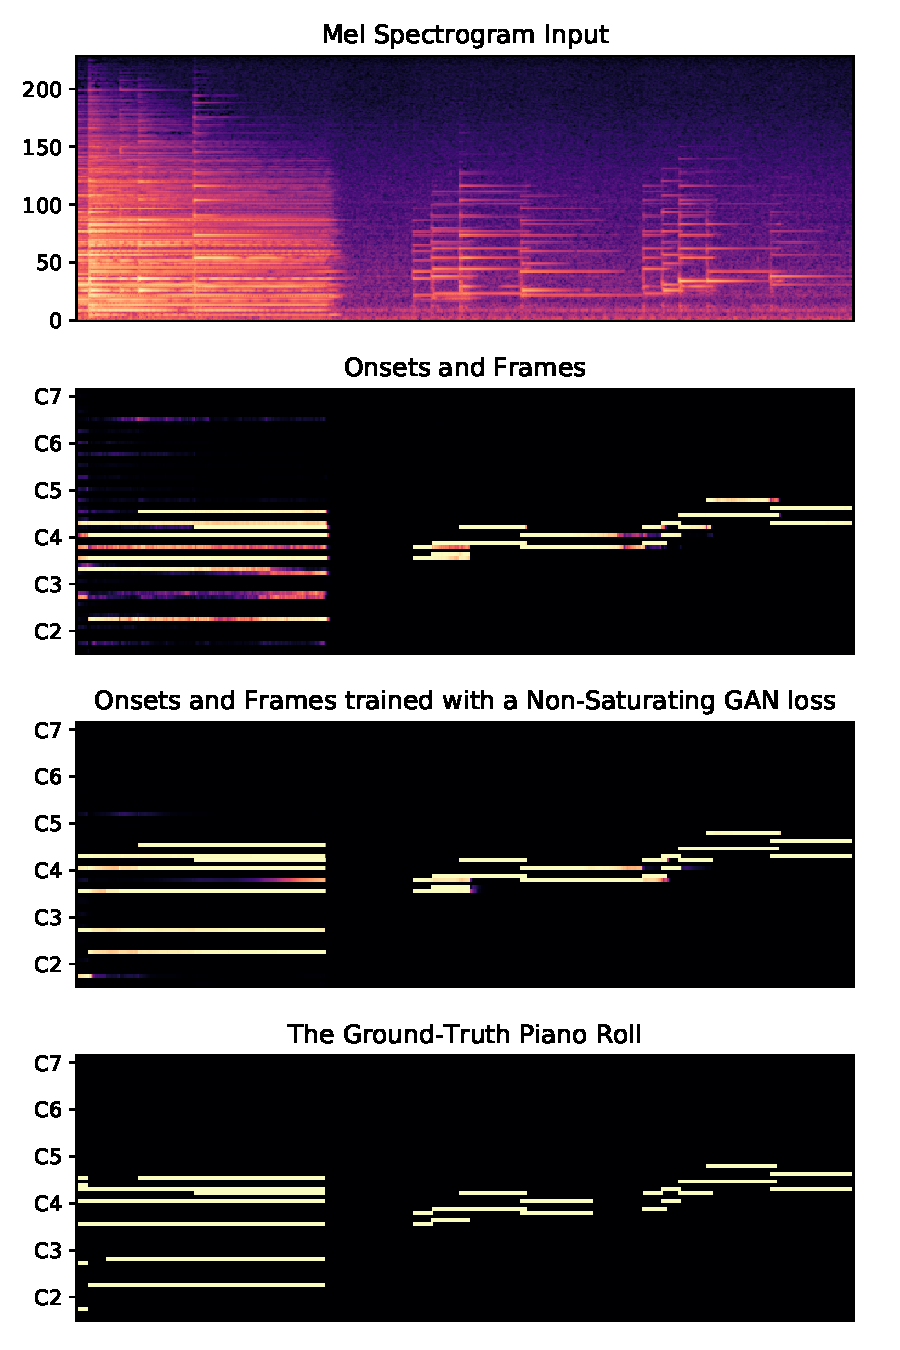
\includegraphics[width=0.499\textwidth]{predictions-115.pdf}%
	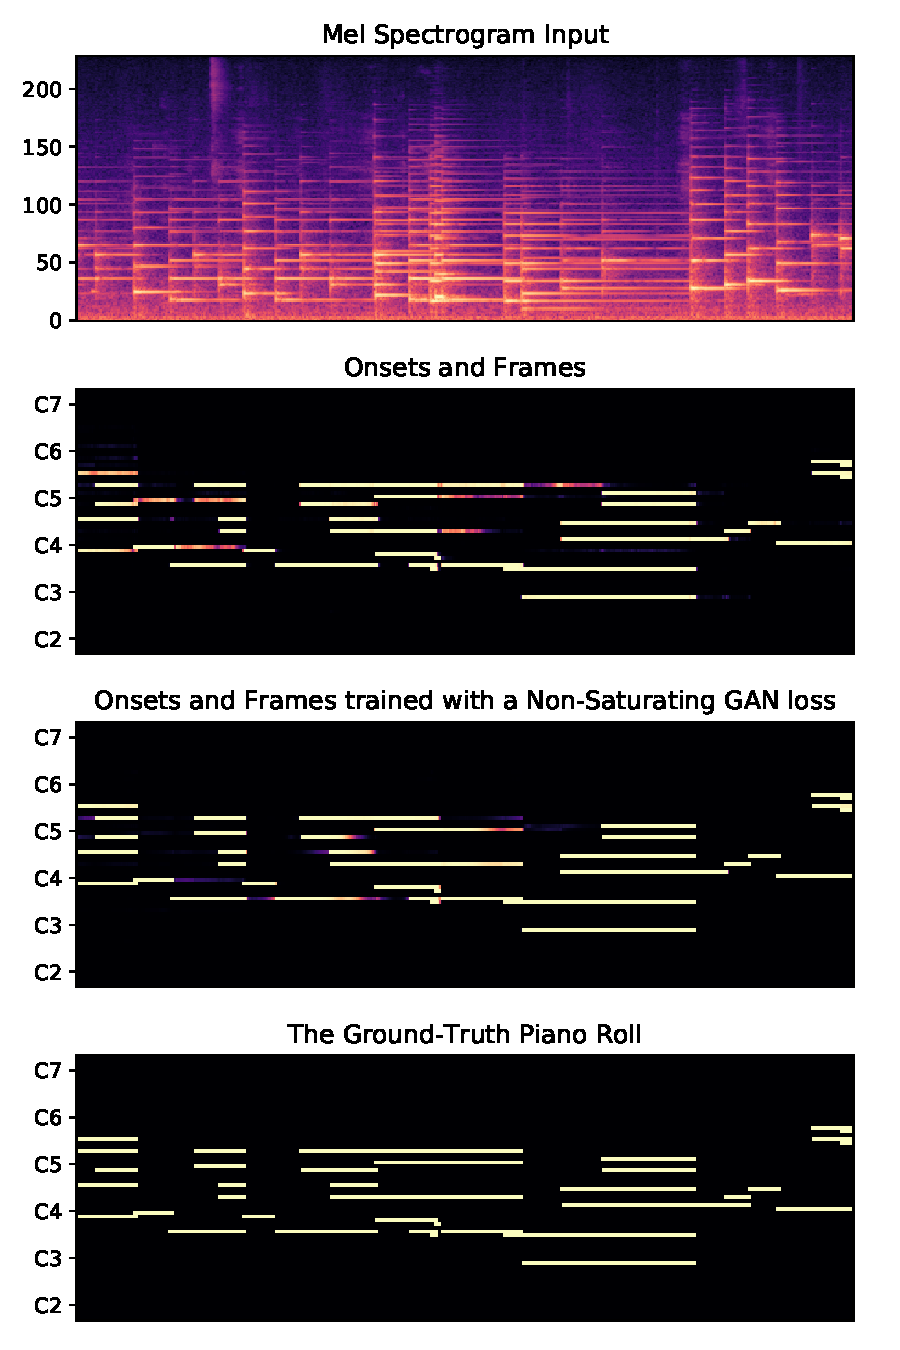
\includegraphics[width=0.499\textwidth]{predictions-73.pdf}%
	%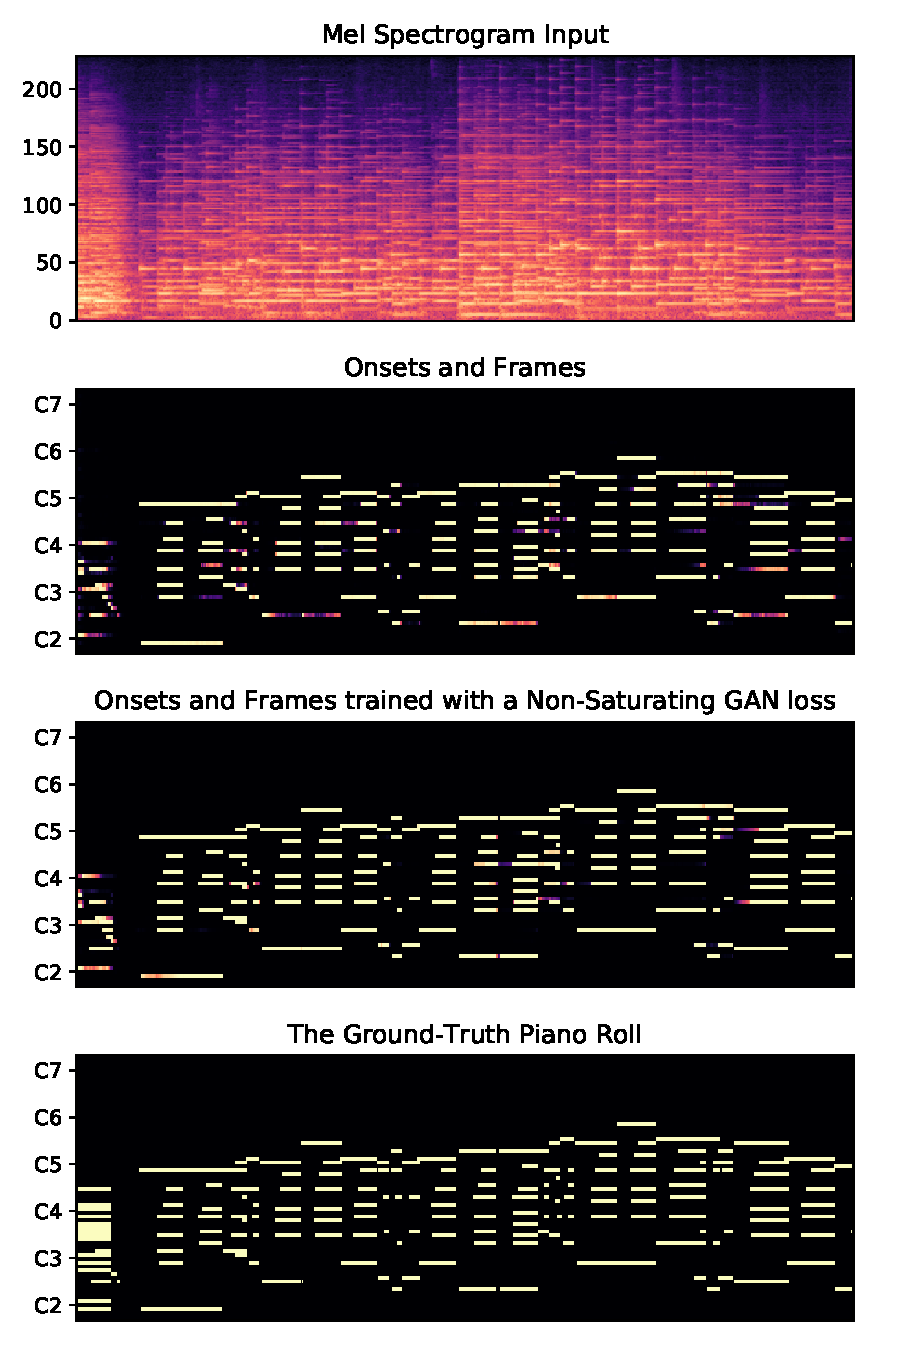
\includegraphics[width=0.333\textwidth]{predictions-64.pdf}%
	\endminipage
	\caption{Comparisons of the frame activation posterior predicted by the baseline and our model ($\ell = \text{BCE}$, $\alpha = 0.3$), on three example segments. The input Mel spectrograms and the target piano rolls are shown together. The GAN version produces more confident predictions compared to the noisy baselines, leading to more accurate predictions.}\label{fig:predictions}
\end{figure*}

\begin{figure*}[t]
	\centering
	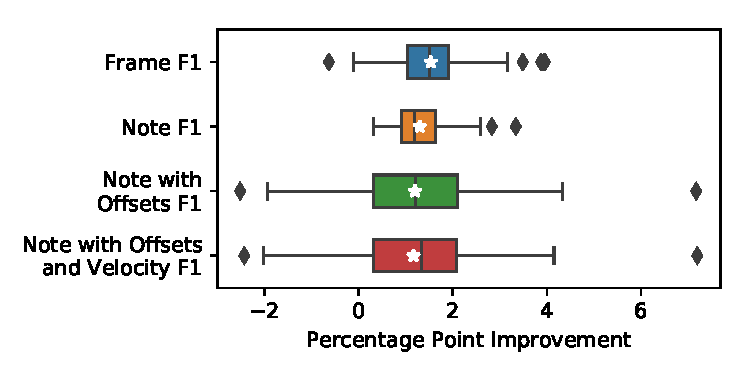
\includegraphics[height=12em]{pertrack.pdf}
	\caption{Distribution of the F1 score improvements over the baseline, tested on the MAESTRO test tracks.}\label{fig:pertrack}
\end{figure*}
\begin{figure*}[t]
	\centering
	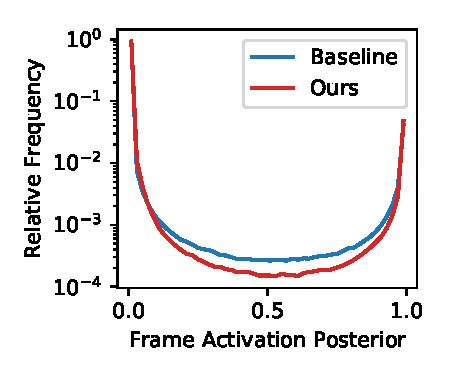
\includegraphics[height=12em]{distribution.pdf}
	\caption{Distribution of frame activation values. Our model outputs more confident predictions, as indicated by the lower relative frequency in (0.1, 0.9).}\label{fig:distribution}
\end{figure*}
\begin{figure*}[t]
	\centering
	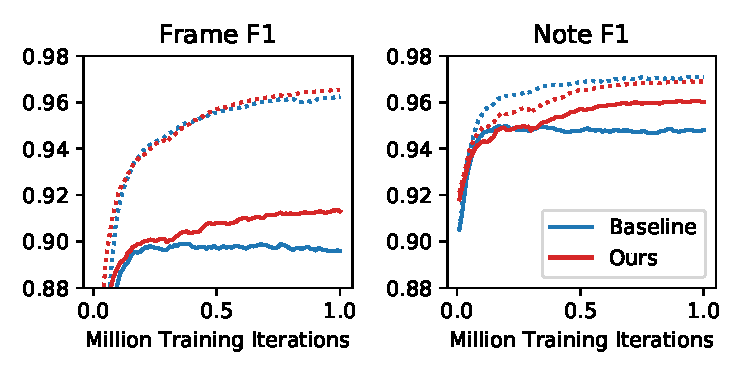
\includegraphics[height=12em]{training.pdf}
	\caption{Learning curves showing the generalization gaps; training curves are drawn as dotted lines, and test curves are drawn as solid lines.}\label{fig:training}
\end{figure*}

Table \ref{tab:alpha} and \ref{tab:performance} summarize the transcription performance, clearly showing a consistent improvement in the conditional GAN models over the Onsets and Frames baseline.
Table \ref{tab:alpha} shows that both non-saturating GAN and least-squares GAN achieve the highest frame and note F1 scores when the \textit{mixup} strength $\alpha = 0.3$ is used, and they both outperform the baseline.
The binary piano rolls are easy to distinguish from the non-binary predictions, which may cause imbalanced adversarial training. \textit{mixup} allows non-binary piano rolls to be fed to the discriminator, making its task more challenging and leading to higher performance.

Table \ref{tab:performance} shows an important trend of the cGAN results compared to the baseline that cGAN trades off a bit of precision for a significant improvement in recall; this is a side effect of the cGAN producing more confident predictions, as will be discussed in the following subsections.

While the percentage differences are moderate, our method achieves statistically significant improvements in F1 metrics on the MAESTRO test dataset ($p < 10^{-14}$ for all 4 metrics, two-tailed paired $t$-test).
The distribution of per-track improvement in each F1 metric is shown in Figure \ref{fig:pertrack}, which indicates that the improvements are evenly distributed across the majority of the tracks.
These improvements are especially promising, considering that Onsets and Frames is already a very strong baseline.

\subsection{Visualization of Frame Activations}

To better understand the inner workings of the conditional GAN framework, we visualize the frame posteriorgrams created by the baseline and the best performing conditional GAN model in Figure \ref{fig:predictions}.
In contrast to the baseline posteriorgrams which have many blurry segments, the posteriorgrams generated by our method mostly contain segments with solid colors, meaning that the model is more confident in its prediction.
Figure~\ref{fig:distribution} shows that the proportion of frame activation values in $(0.1, 0.9)$ is noticeably higher in the baseline, thus making the output less sensitive to the threshold choice.
This is because indecisive predictions are penalized by the discriminator, since they are easy to distinguish from the ground-truth which contains only binary labels.
The generator is therefore encouraged to output the most probable note sequences even when it is unsure, rather than producing blurry posteriorgrams that might hamper the decoding process.
This allows for an interpretation in which the GAN loss provides a prior for valid onset and frame activations, and the model learns to perform MAP estimation based on this prior.


\subsection{Training Dynamics and The Generalization Gap}

Figure \ref{fig:training} shows the learning curves for the frame F1 and note F1 scores, where the scores on the training dataset are plotted in dotted lines.
It is noticeable in the figure that the validation F1 scores for the baseline stagnate after 300k iterations, while the F1 scores of our model steadily grow until the end of 1 million iterations.
Thanks to this, the generalization gap --- the difference between the training and validation F1 scores --- is significantly smaller for the conditional GAN model.
This means that the GAN loss works as an effective regularizer that encourages the trained model to generalize better to unseen data, rather than memorizing the note sequences in the training dataset as LSTMs are known to be capable of~\cite{zaremba2015recurrent}.

\section{Conclusions}

We have presented an adversarial training method that can consistently outperform the baseline Onsets and Frames model, using the standard frame-level and note-level transcription metrics and visualizations that show how the improved model predicts more confident output.
To achieve this, a discriminator network is trained competitively with the transcription model, i.e. a conditional generator, so that the discriminator serves as a learned regularizer that provides a prior for realistic note sequences.
After training, the discriminator can be disregarded for inference, incurring no additional computational cost during transcription.


Our results show that modeling the inter-label dependencies in the target distribution is important and brings measurable performance improvements.
Our method is generic, and any model that involves predicting two-dimensional representation should be able to benefit from including an adversarial loss.
These approaches are common not only in transcription models but also in speech or music synthesis models that predict spectrograms as an intermediate representation~\cite{shen2018tacotron,kim2019synthesis}.
This implies that the findings in this chapter is applicable to a broader set of problems not only in multi-pitch estimation but also in the field of music information retrieval in general.

Our results do not include the effects of using data augmentation~\cite{hawthorne2019maestro}, which is orthogonal to our approach and should bring additional performance improvements when applied.
As discussed, the discriminator imposes the prior on the target domain whereas data augmentation enriches the input audio distribution.
This implies that our method would be less effective when the majority of errors are due to the discrepancy in the audio distribution between the training and test datasets.
How to apply adversarial learning for better generalization on the input distribution is a potential future research direction.

We have argued that the adversarial discriminator serves as a regularizer providing the prior knowledge of how the note sequences in the dataset should look like, which complements the conditionally independent output of the Onsets and Frames model.
The fully-connected output layer also does not take into account a very important characteristic of pitch, that each pitch corresponds to quasi-periodic signals in the input with a known frequency that are geometrically spaced --- rather, the predictions are instead made as if each pitch is completely independent pieces of information, not utilizing the knowledge on pitch at all.
Another important concept that is not considered in this chapter is the timbre.
Although the MAESTRO dataset used in this chapter contains various recording conditions and therefore somewhat different timbres among the tracks, they are all recordings of piano performances which have limited timbral diversity.
These aspects motivate building an improved model that can leverage the regularity of pitch as well as the knowledge of instrumental timbres.
In the next chapter, we discuss how to extend our music transcription model to incorporate such aspects, specifically by using a synthesizer model similar to the one used in Chapter \ref{ch:synthesis}.

%!TEX root = ../dissertation.tex
% this file is called up by thesis.tex
% content in this file will be fed into the main document

\graphicspath{{7-timbre/figures/}}

\chapter{Synthesizer-Aided Multi-Instrument Transcription}
\label{ch:timbre}

In Chapter \ref{ch:introduction}, we introduced the idea of extending a music transcription model with an additional synthesizer component that can convert the transcribed information back to the input audio, forming an analysis/synthesis framework as depicted in the encoder-decoder architecture in Figure \ref{fig:autoencoder}.
By doing so, we anticipated that the two components --- the transcriber and the synthesizer --- can work together to better translate information between the two representations, i.e. audio waveform and the transcribed semantic information of the music.
One motivation for employing such analysis/synthesis framework is that the advent of many successful deep learning techniques and the improved hardware capability may allow us to convert an audio signal completely into the constituent pieces of musical information that we want to transcribe, that are entangled in an extremely sophisticated way in the audio signal.
In the preceding chapters, we have considered deep learning solutions to various problems in music analysis and synthesis, such as monophonic pitch tracking (Chapter \ref{ch:monophonic}), music synthesis with controllable timbre (Chapter \ref{ch:synthesis}), and polyphonic music transcription (Chapter \ref{ch:adversarial}).
These problems correspond to a certain subset of the full encoder-decoder architecture, and in each chapter we discussed how the design choices in the model architecture and dataset construction affect the experimental results and the real-world applicability.

Having learned the lessons from these, in this chapter we aim to construct an automatic music transcription system that encompasses the full analysis/synthesis cycle, by considering the general problem of multi-instrument polyphonic music transcription.
We propose an autoencoder architecture that appends a synthesis model on top of a transcription model, and we verify the effects of the appended synthesizer in the experiments.
As in Chapter \ref{ch:synthesis}, the synthesizer component is capable of capturing the different aspects of various timbres in the dataset using a learned timbre space representation.
We show that the synthesizer component can serve as a regularizer to the transcriber, providing a form of prior knowledge on the spectral and temporal characteristics of the timbres. 
% \TODO{some conclusive sentence summarizing the results of this chapter}

\section{Introduction}

Multi-instrument music transcription aims to extract not only the occurrences of multiple simultaneous pitches and notes but also the types of one or more instruments corresponding to those notes.
Since it poses additional challenges to the already difficult problem of polyphonic music transcription, studies on the complete multi-instrument polyphonic transcription problem are relatively rare.
Instead, most studies on analyzing multi-instrument audio focus on either developing a discriminative model for polyphonic where timbre information is disregarded~\cite{bittner2017deepsalience} %\TODO{cite more}
or the problem of instrument recognition, while not identifying the individual notes that belongs to the recognized instruments~\cite{lostanlen2016spiral}. %\TODO{cite more}
To take both polyphonic notes and multiple instruments into account, a model has to carefully incorporate the prior knowledge of how pitch and timbre are reflected in the audio signal, e.g. using a probabilistic latent component model~\cite{benetos2015probabilistic} or a variant of non-negative matrix factorization~\cite{grindlay2009eigeninstruments}.
To produce outputs in multiple domains, these models have to include an intricate set of design choices to implement a mathematical representation of the prior knowledge.

Meanwhile, the main premise of deep learning is quite opposite of how those models are designed.
Rather than writing down the set of rules manually, layers of simple calculations can serve as a very effective function approximator, that can produce just about anything when an enough amount of data is fed to the black box.
In these models, the prior knowledge baked into the model architecture is minimal.
Take the Onsets and Frames model~\cite{hawthorne2018onsetsframes} for example; the model output has 88 dimensions corresponding to each key of the piano, but the 88 keys are treated as a separate multi-label target, without utilizing the knowledge that each key should represent a certain frequency that the quasi-periodic signal in the input follows.
Because of this lack of ``inductive bias'', deep learning models typically have to be trained with a very large amount of data; in other words, they are less sample efficient.


Generative models for transcription, such as a Bayesian network representation of spectrogram~\cite{bergkirkpatrick2014unsupervised}, takes the opposite approach.
These models define the process of generating sound entirely from the parameterized sources that typically convey a physical interpretation, such as the modeling of attack-decay-sustain-release (ADSR) curves or the energy distribution along harmonics. 
Compared to data-driven models with a lot of learnable parameters, however, those interpretable transcription models often lack the flexibility to be applicable for a wider variety of inputs.

In this chapter, we explore the possibility of finding a compromise between the two extremes.
Specifically, we examine how to induce the transcription model to make predictions such that, when synthesized back into audio, resemble the original audio input.
We do this by appending a neural music synthesis model to the transcription model, and the synthesis model is specifically designed to describe the sound generation process with a small number of interpretable parameters, which is restrictive enough to guide the transcription model to more accurate predictions, yet flexible enough to be learnable in a data-driven manner.
We evaluate this approach with a multi-instrument transcription task and show that a synthesis model can serve as an effective regularizer. % \TODO{describe qualitative improvement}

\section{Related Work}


\subsection{Multi-Instrument Music Transcription}

Transcribing polyphonic music with multiple instruments present is a particularly difficult problem and there has been relatively few successful attempts, as it requires solutions to instrument classification in addition to multiple pitch estimation.
While some approaches perform source separation and instrument recognition as a separate pre-processing step for per-instrument polyphonic transcription,~\cite{heittola2009separation,itoyama2011bayesian}, a number of approaches attempt to jointly solve the two problems, by modeling possible instruments as a constraint to non-negative matrix factorization (NMF)~\cite{grindlay2009eigeninstruments}, applying spectral templates to a probabilistic latent component model~\cite{benetos2015probabilistic}, and using a U-Net architecture to separate a multi-channel representation of audio into per-instrument transcriptions~\cite{wu2019musicnet}.
In general, joint estimation of instrument and multiple pitches allows for flexible modeling of diverse sounds and enables an end-to-end approach for multi-instrument polyphonic transcription.


\subsection{Deep Clustering}

Deep clustering~\cite{hershey2016deepclustering} is a technique for audio source separation which learns a mapping from each time-frequency bin of the input audio into an embedding space.
% During training, a pair of embedding vectors corresponding to the same source are encouraged to be closer to each other, while pushing the pairs corresponding to different sources apart from each other. To do this, 
The original formulation uses the class assignment matrix $Y = \{ y_{i,c} \}$ indicating whether element $i$ belongs to cluster $c$ and learns the embedding matrix $V = \{ \mathbf{v}_{i} \}$ as a function of the input audio that minimizes the Frobenius distance between the assignment matrix:
\begin{equation}\label{eqn:deepclustering}
\mathcal{L} = \lVert VV^\top - YY^\top \rVert_{\mathrm{F}}^2 = \sum_{i, j} \left ( \left < \mathbf{v}_i, \mathbf{v}_j \right > - \left < \mathbf{y}_i, \mathbf{y}_j \right > \right )^2.
\end{equation}
Since $\left < \mathbf{y}_i, \mathbf{y}_j \right >$ equals 1 if the elements $i$ and $j$ belongs to the same cluster and 0 otherwise, the learned embedding vectors are optimized to be as close as possible for the vectors which belong to the same cluster and as orthogonal as possible otherwise.
Alternative objective functions to Equation \ref{eqn:deepclustering} employing deep neural networks have been suggested by~\cite{wang2018deepclustering}.
The deep clustering technique has been successfully applied to the multi-speaker separation~\cite{isik2016deepclustering} and the singing voice separation problem~\cite{luo2017deepclustering}.

This chapter's work borrows the idea of deep clustering and builds an embedding space that captures the timbres of different instruments, while relying on a synthesizer component rather than inducing every pair of embedding vectors to be orthogonal to each other.
By allowing different embedding vectors to be similar but not necessarily orthogonal, the synthesizer can learn to map similar-sounding instruments to vectors that are close to each other.
Informed by this embedding space, the multi-instrument transcription model can more easily learn to classify the similar instruments than when the instruments are treated independently.


% \subsection{Source-Filter Synthesis}
% \cite{heittola2009separation} (instrument recognition)

\subsection{Generative Modeling for Transcription}

Bayesian approaches for music transcription consider the audio generation process as a probabilistic model that can describe the generated audio in terms of its sound events.
In these approaches, an audio representation such as a spectrogram is considered as an observation, and the model parameters that maximizes the observation is found using Bayesian inference techniques such as particle filtering~\cite{dubois2005harmonic}, message propagation~\cite{cemgil2006generative}, and block-coordinate ascent~\cite{bergkirkpatrick2014unsupervised}.
These models typically work well for small test datasets with a homogeneous timbral profile, but because they rely on a small, manually designed set of parameters for sound generation, they often struggle to generalize to diverse inputs.

In the spirit of utilizing the synthesizer component for transcription,
\citeA{li2017infinite} explored the idea of using on-the-fly synthesized training dataset for piano transcription, using a simple fully-connected neural network operating on the CQT representation.
\cite{choi2019drum} proposes appending a drum synthesizer component to enable fully unsupervised training of drum transcription.
The work in this chapter draws several ideas from these previous approaches of incorporating a synthesizer component into the loop, while also leveraging the flexibility and the generalizability of data-driven deep learning.

\section{Method}

We first describe the synthesizer model, followed by the modifications to the Onsets and Frames~\cite{hawthorne2018onsetsframes} transcription model made to allow the concatenation of the two models.

\subsection{Synthesizer Model}

The synthesizer model takes a per-instrument piano roll representation of symbolic music (see Figure \ref{fig:transcription-to-piano-rolls}) and uses a learned instrument embedding to predict the Mel spectrogram of the corresponding audio.
We are assuming here that predicting Mel spectrograms is equivalent to synthesizing the audio for our purposes, since we have seen in Chapter \ref{ch:synthesis} that Mel spectrograms contain most of the perceivable information present in the audio content, and the original audio can readily be reconstructed using sample-based synthesis models like WaveNet~\cite{oord2016wavenet}.

The synthesizer consists of two subcomponents, the envelope estimator and the waveshaper, respectively implementing the temporal and spectral characteristics of the sound being synthesized.
The computation in each subcomponent is performed independently for each pitch-instrument combinations, and their results are combined to obtain the resulting Mel spectrogram, as shown in Figure \ref{fig:synthesizer-architecture}.
Both components take the instrument embedding in order for the synthesized audio to exhibit different temporal and spectral behaviors depending on the instrument, and together they ensure that the synthesis model only creates harmonic sounds with the frequency corresponding to the pitch of input notes and the spectral envelope consistent among each instrument.

The envelope estimator component predicts the temporal envelope of each note, by mapping the note activities into a latent space using a one-dimensional convolution layer, followed by a FiLM layer~\cite{perez2018film} to condition on the instrument.
A GRU layer~\cite{cho2014seq2seq} is then applied in order to model the temporal behavior, such as the attack-decay-sustain-release (ADSR) curves.
Meanwhile, the waveshaper component performs a subtractive synthesis to obtain the spectrum corresponding to each pitch and instrument.
We use two types of source waves, sawtooth and triangular, to make it easily adaptable to the timbres that primarily consists of odd harmonics, such as the clarinet.
The instrument embedding is used to predict the transfer function in the Mel frequency domain to be applied to each source spectrum, which is modeled as a polynomial function mapping Mel frequencies to log magnitudes.
The Mel spectrogram corresponding to each note can then be calculated in the complex domain, by assigning a random initial phase to each pitch-instrument pair and multiplying the temporal envelope predicted by the envelope estimator.
All of the per-note Mel spectrograms are then added to obtain the final Mel spectrogram output.



\begin{figure}
	\centering
	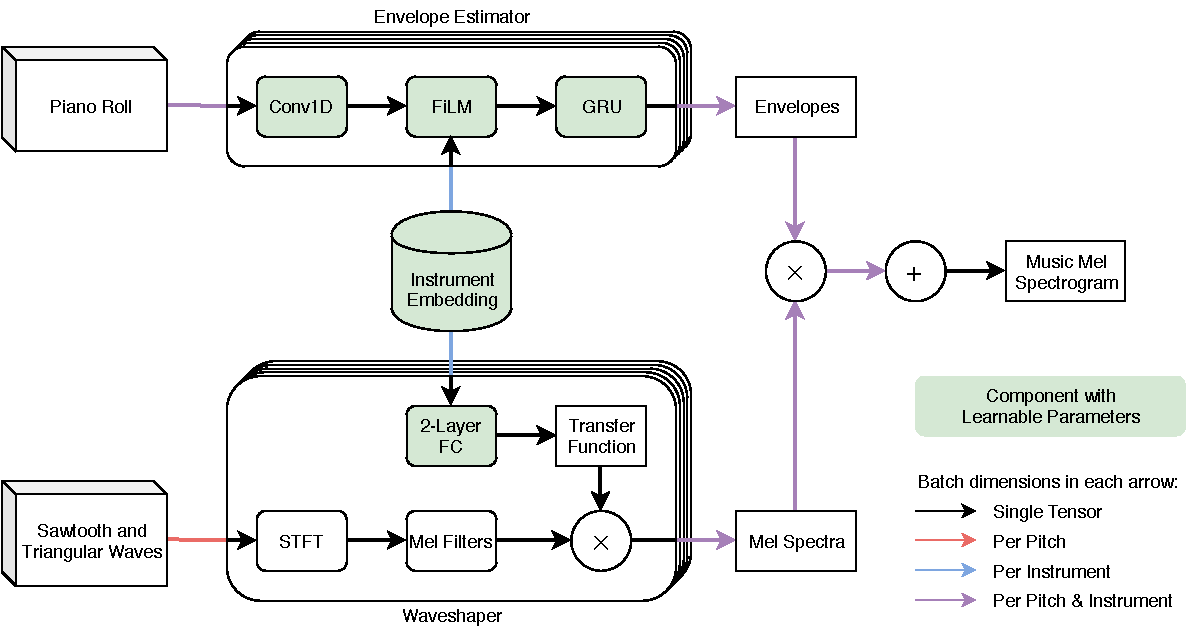
\includegraphics[width=\textwidth]{synthesizer-architecture.pdf}
	\caption{The synthesizer architecture. The temporal and spectral characteristics of each notes are respectively modeled by the envelope estimator and the waveshaper. This structure enforces each instrument to have consistent spectral and temporal envelopes across the pitch.}\label{fig:synthesizer-architecture}
\end{figure}


\subsection{Training Transcriber with Appended Synthesizer}

To append the synthesizer component to the output of the transcription model while keeping the full model differentiable, we expand the fully-connected layer predicting the frame activation to additionally predict the instrument embedding corresponding to each time-frequency bin.
Using the expanded outputs, the frame activations and the predicted embedding can be fed to the synthesizer component.
The frame activations are binarized before feeding to the synthesizer, and we use a gradient-stop for this connection.

The synthesizer model is separately trained, and the transcriber model is then optimized to minimize the sum of three losses:
\begin{equation}
\mathcal{L}_{\text{Overall}} = \mathcal{L}_{\text{Onsets \& Frames}} + \lambda \left ( \mathcal{L}_{\text{Embedding}} + \mathcal{L}_{\text{Synthesizer}} \right )
\end{equation}
The first term, $\mathcal{L}_{\text{Onsets \& Frames}}$, is the loss of the Onsets and Frames model which is the sum of the binary cross entropy of the onsets, offsets, and frame predictions.
We define $\mathcal{L}_{\text{Embedding}}$ as the mean squared error (MSE) between the predicted instrument embedding and the ground truth, and $\mathcal{L}_{\text{Synthesizer}}$ is defined as the mean cosine distance between the predicted and the ground-truth Mel spectra:
\begin{equation}
\mathcal{L}_{\text{Synthesizer}} = \mathbb{E}_{\hat{\mathbf{s}}, \mathbf{s}} \left [ 1 - \frac{ \hat{\mathbf{s}} \cdot \mathbf{s} }{\lVert \hat{\mathbf{s}} \rVert \lVert \mathbf{s} \rVert} \right ]
\end{equation}
where $\mathbf{s}$ follows the distribution of Mel spectra in the input audio, and $\hat{\mathbf{s}}$ is the Mel spectra predicted by the synthesizer based on the transcription predicted from $\mathbf{s}$.

\section{Experimental Setup}

We use the MusicNet dataset~\cite{thickstun2017musicnet} to train both the synthesizer and the transcriber.
The dataset contains 2,048 minutes of classical chamber music audio and labels, which comprises 330 recordings of various ensembles.
The dataset contains annotations of 11 General MIDI instruments: Acoustic Grand Piano, Harpsichord, Violin, Viola, Cello, Contrabass, French Horn, Oboe, Bassoon, Clarinet, and Flute.
Different recordings in the dataset have drastically different tuning, ranging more than a semitone in some recordings which would result in a wrong transcription even by a perfect transcriber.
To alleviate this, we preprocess the dataset by running a tuning estimator implemented in librosa~\cite{mcfee2015librosa} on each track and pitch-shifted any recordings that are more than 20 cents apart from the A440 tuning.

Unlike in Chapter~\ref{ch:adversarial}, we use the original Onsets and Frames model size of 512, and the transcription model contains 10 million parameters.
We use a 2-dimensional instrument embedding space to represent the distribution of the 11 instruments, and the polynomial transfer functions used in the subtractive synthesis are modeled by cubic B\'{e}zier curves.


The audio is resampled to 16kHz, and a training batch is composed of eight 20-second audio segments and labels.
We use Adam optimizer~\cite{kingma2015adam} with learning rate 0.0006, and the learning rate decay of factor 0.98 is applied every 1000 steps.
We ran the optimization for 180,000 steps and report the transcription accuracy evaluated on the 10 test recordings provided in the MusicNet dataset.

\section{Results}

\subsection{Synthesizer Output}

\begin{figure}
\centering
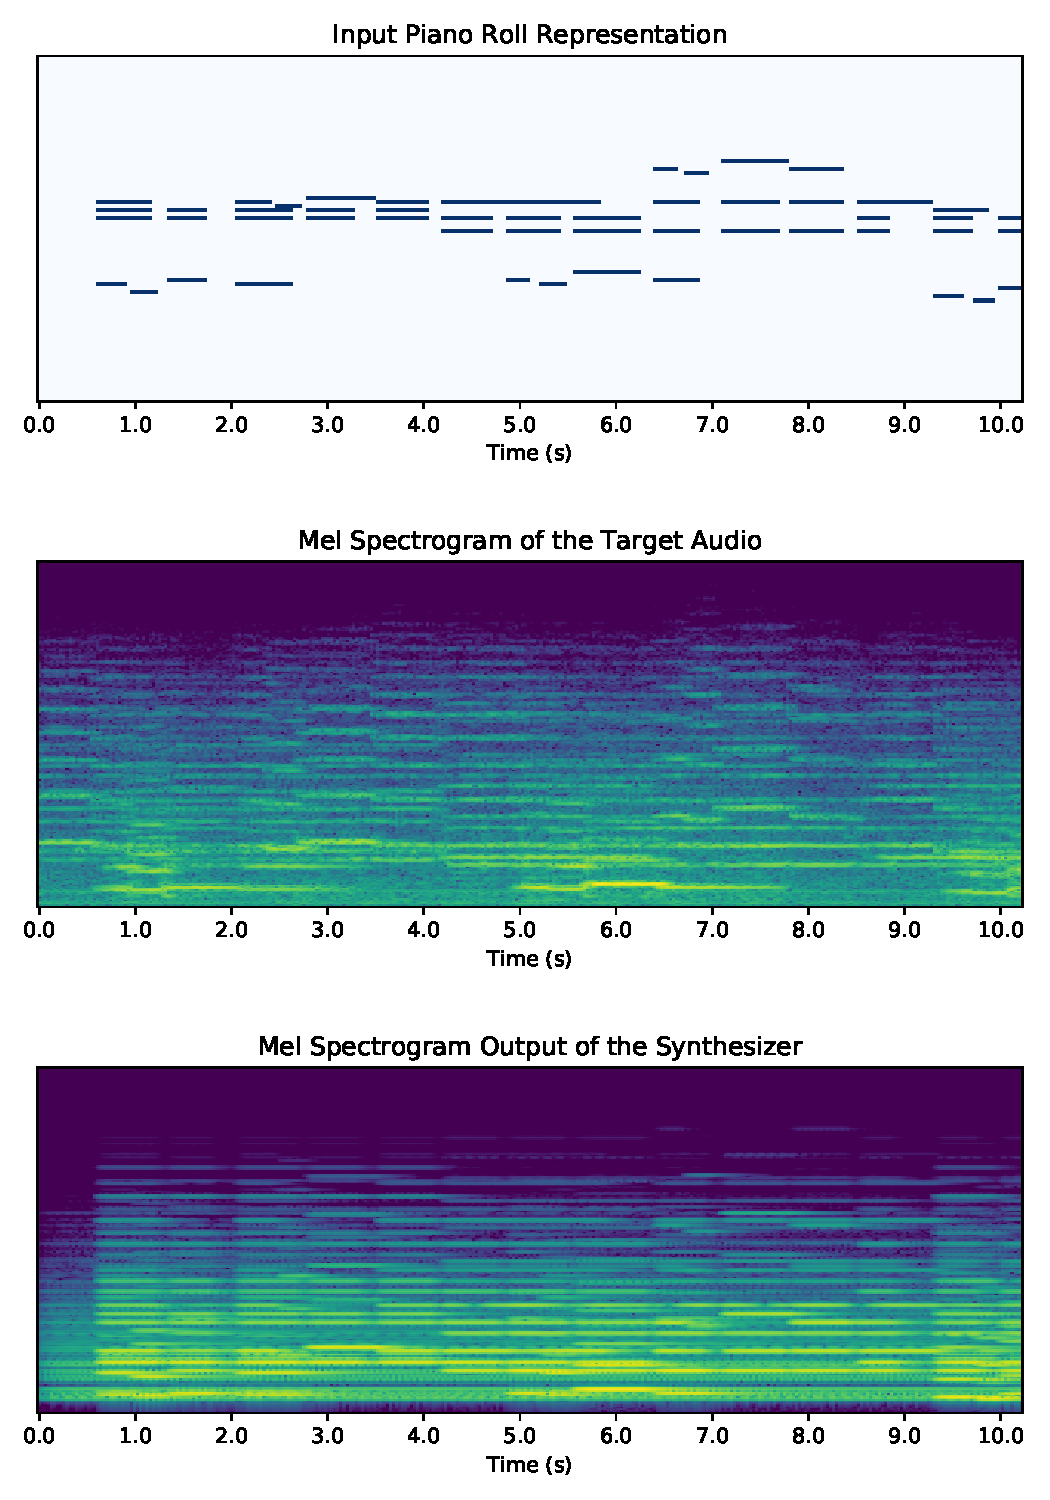
\includegraphics[width=\textwidth]{synthesizer-output.pdf}
\caption{An example of the input, target, and output representations of the synthesizer. The output resembles the target Mel spectrogram but shows a regular pattern as constrained by the synthesizer model.}\label{fig:synthesizer-output}
\end{figure}

Figure \ref{fig:synthesizer-output}: the synthesizer output

\subsection{Transcription Accuracy}

\begin{figure}
\centering
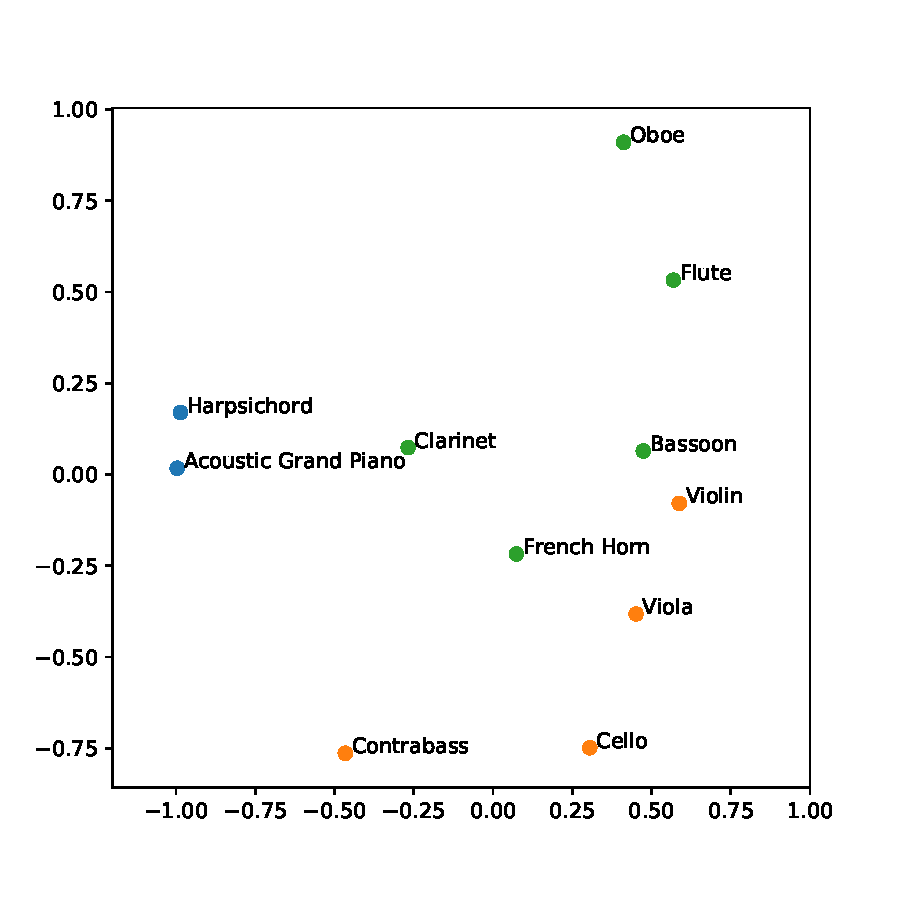
\includegraphics[width=0.7\textwidth]{cosine_distance.pdf}
\caption{The learned timbre embedding space mapping the 11 instruments in the MusicNet dataset into the corresponding points in the space. Types of instruments (keyboards, winds, and strings) are color-coded.}\label{fig:learned-timbre-embedding}
\end{figure}

\begin{itemize}
	\item Figure~\ref{fig:learned-timbre-embedding}: learned timbre embedding
	\item Table~\ref{tab:transcription-accuracy-comparison}: accuracy comparison
	\item \TODO{Error Analysis}
\end{itemize}

The multi-label baseline exhibits significantly lower performance in these instrument-agnostic metrics, and the proposed model slightly outperforms the single-label baseline, which does not predict the instrument labels.

\begin{table}
\centering\small
\begin{tabular}{c|ccc}
& \makecell{Baseline \\ (single label)} & \makecell{Baseline \\ (multi-label)} & \makecell{Synthesizer-aided \\ (ours)} \\ \hline
Precision & 0.736 & 0.714 & 0.735 \\ 
Recall & 0.711 & 0.600 & 0.726 \\ 
F1 Score & 0.720 & 0.650 & 0.729 \\
\end{tabular}
\vspace{1em}
\caption{A comparison of instrument-agnostic frame transcription accuracies for the baseline models and the proposed synthesizer-aided transcription model. The proposed model achieves better recall while staying at the same precision.}\label{tab:transcription-accuracy-comparison}
\end{table}

\subsection{Multi-Instrument Transcription}

\TODO{multi-instrument accuracy}

\subsection{MusicNet Inspector}

\begin{figure}
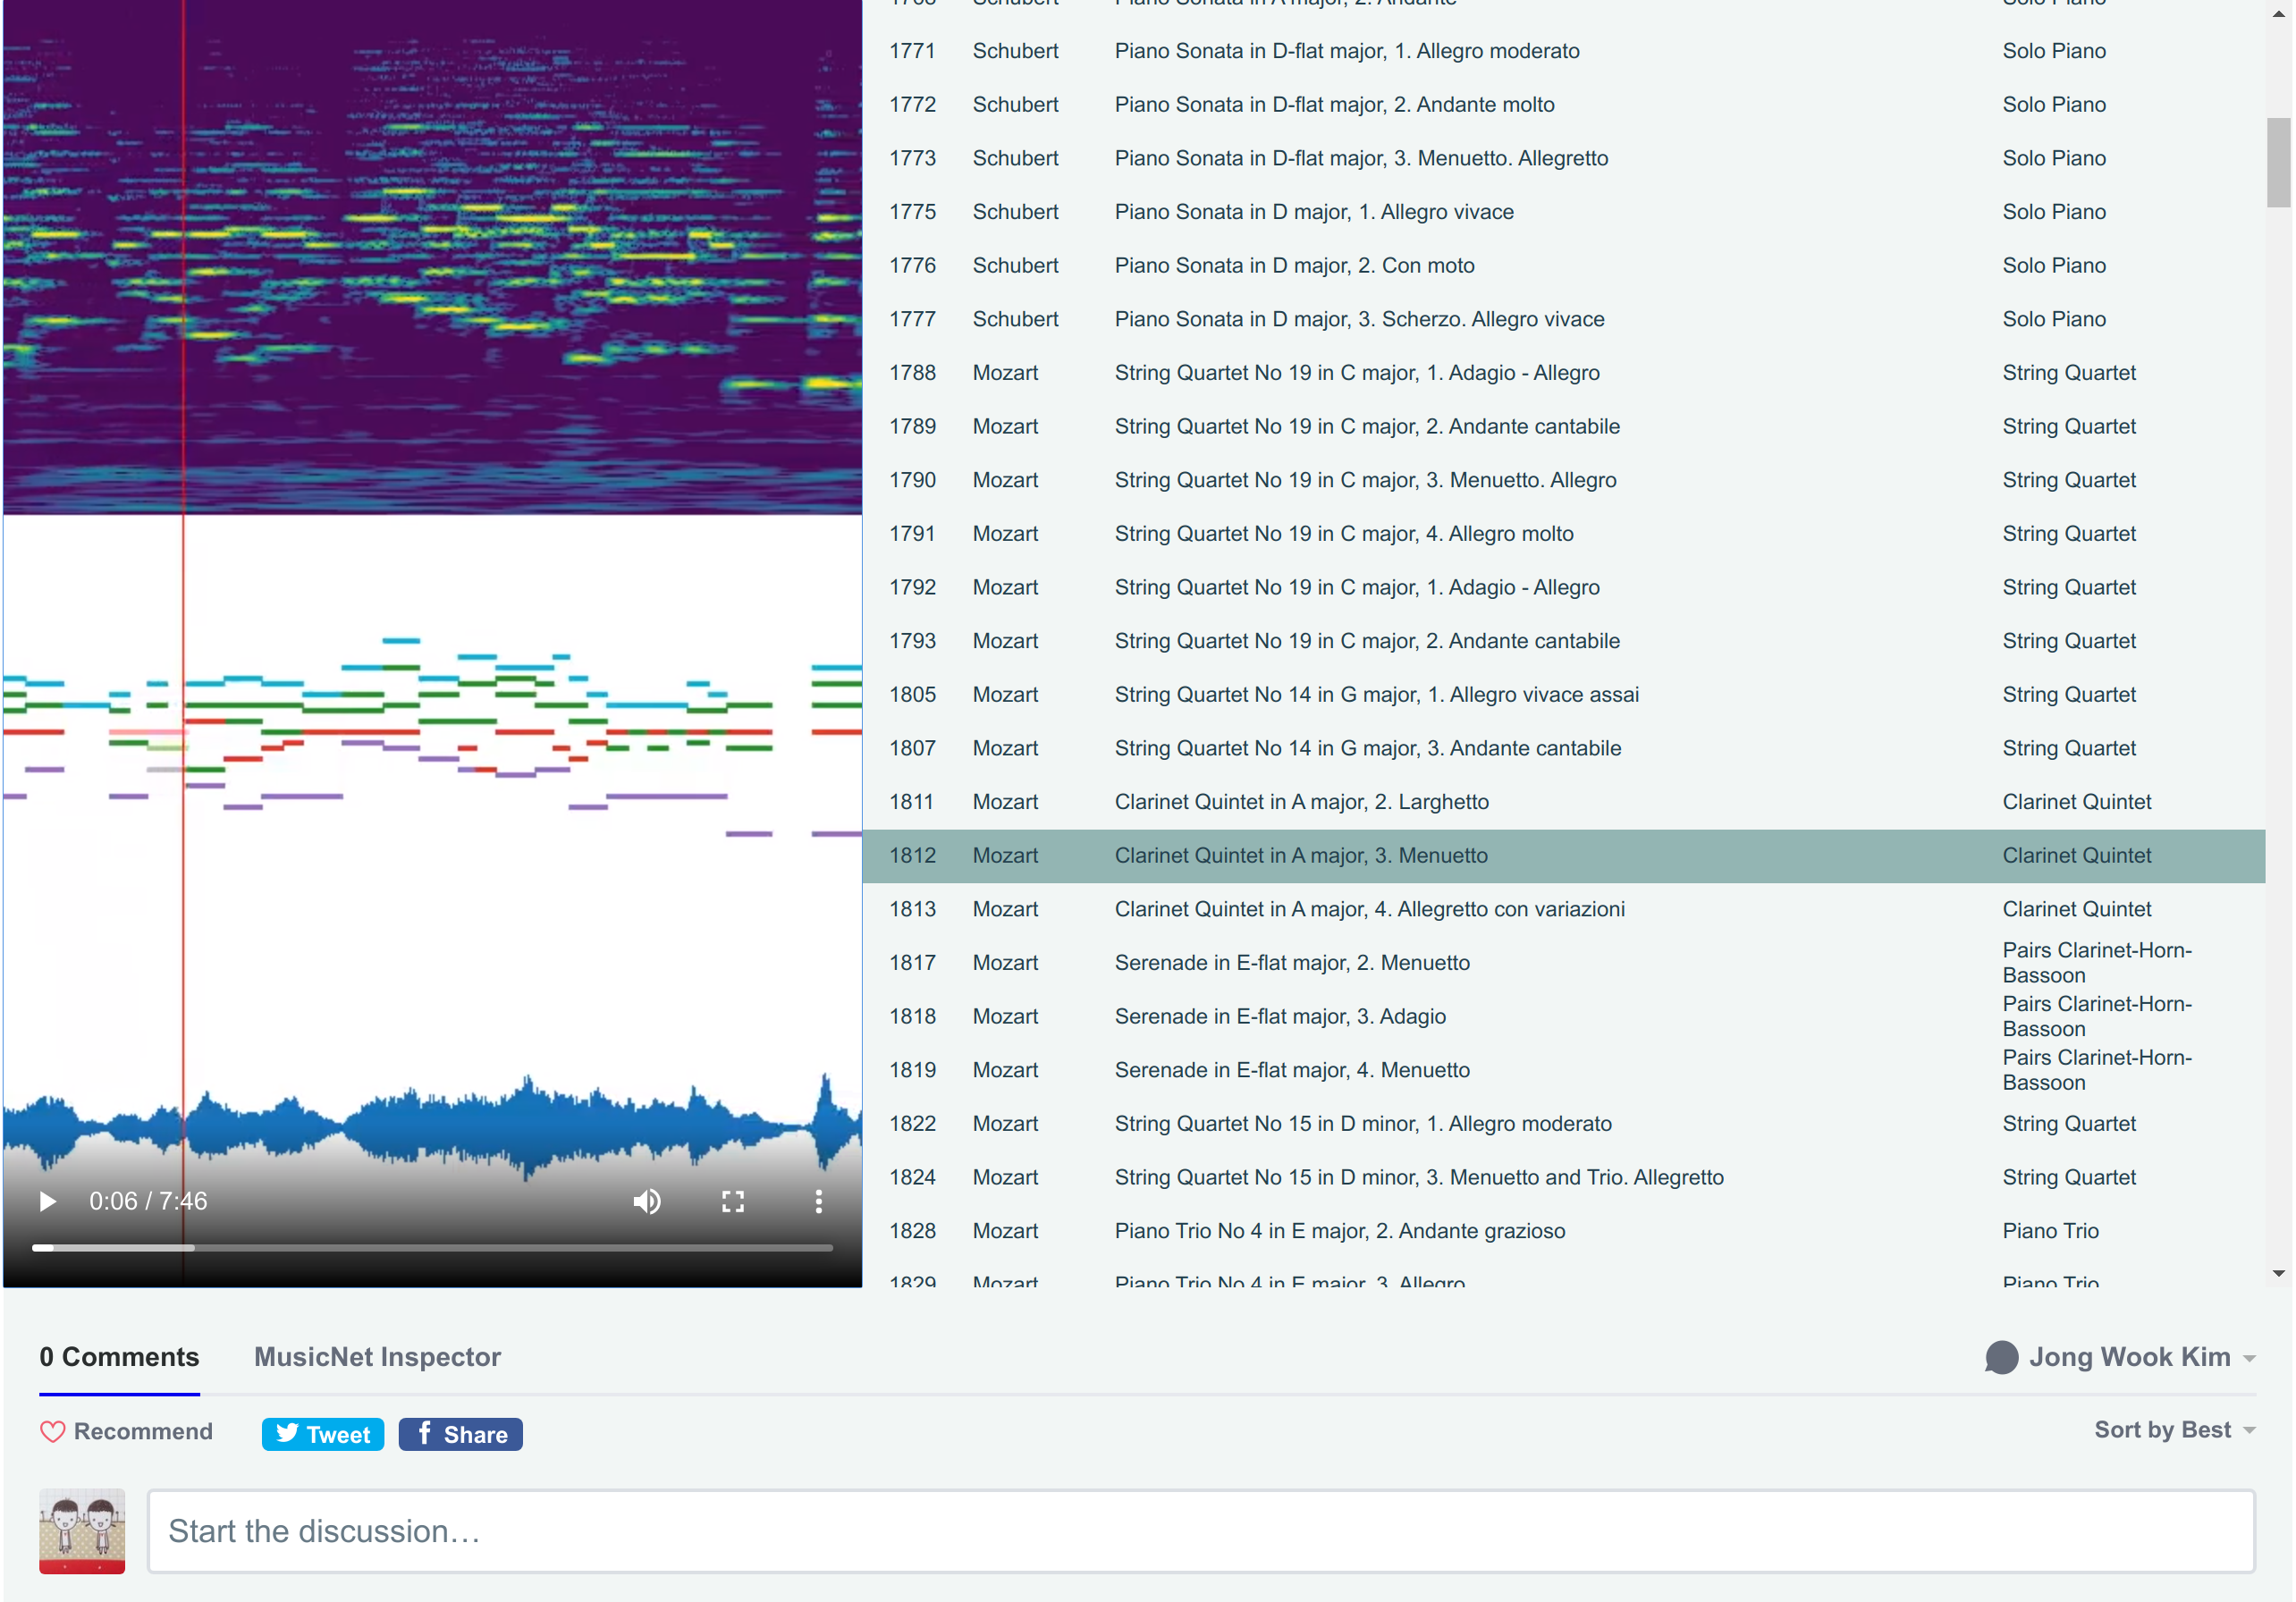
\includegraphics[width=\textwidth]{inspector.png}
\caption{The MusicNet Inspector web interface. Users can select among the 330 tracks in the MusicNet dataset, and the selected track is played together with the CQT, piano roll, and amplitude visualizations.}\label{fig:musicnet-inspector}
\end{figure}

Figure~\ref{fig:musicnet-inspector}: the web UI.

\section{Conclusion}

\begin{itemize}
	\item Discussion points: dataset quality, unison, dot product space, Lipschitz; volume information, inharmonicity
\end{itemize}


%!TEX root = ../dissertation.tex
% this file is called up by thesis.tex
% content in this file will be fed into the main document

\graphicspath{{8-conclusions/figures/}}

\chapter{Conclusions and Final Remarks}
\label{ch:conclusions}

\section{Summary}

\section{Takeaways}

\begin{itemize}
	\item Dataset matters (highly correlated than images ~\cite{thickstun2018invariances})
	\item Prior knowledge matters in all domains
\end{itemize}


\section{Future Research Directions}

\begin{itemize}
	\item fully-fledged synthesis model
	\item sound as discrete events
	\item transcriptional turing test
\end{itemize}


%: ----------------------- bibliography ------------------------
{
\hypersetup{linkcolor = RoyalBlue}
\onehalfspacing
\renewcommand\bibname{Bibliography}
\renewcommand\bibliographytypesize{\small}
\bibliography{library/library}
}

%: ----------------------- appendices --------------------------
% \appendixbegin
% \appendix

\chapter{Brownie tootsie roll lollipop cookie}
\label{adx:a}

\doublespacing

Oat cake pudding sweet lemon drops gummies cookie. 
Dragee lollipop ice cream apple pie sweet roll brownie. 
Lollipop marshmallow jelly beans marzipan sugar plum chupa chups caramels toffee. 
Croissant icing chocolate cake oat cake muffin powder tart. 
Croissant wafer dessert pudding cupcake croissant. 
Cheesecake wafer sugar plum danish. 
Liquorice powder sesame snaps.


%: --------------------------- index ---------------------------
% \clearpage
% \begin{footnotesize}
% \cleardoublepage % ensure the right page
% \phantomsection % sets an anchor
% \printindex
% \end{footnotesize}

\end{document}
